%:Clase del documento
\documentclass[fontsize=10pt, Myfinal=true, twoside, numbers=noenddot]{scrbook}
%, Myfinal=true, Minion=true, English=true

%:Paquete de estilos propuesto
\usepackage{libroETSI}

%:Paquete específico para cargar tikz (y sus librerías) y pgfplots
\usepackage{dtsc-creafig}

%:Paquete para notaciones específicas
\usepackage{notacion}

%:Paquete para incorporar aspectos concretos de la edición
\usepackage{edicionTesis}

%:Estas líneas de código son INNECESARIAS excepto para mostrar determinadas características en este manual. Pueden eliminarse o comentarse sin ningún problema.
%Se usan para compilar el capítulo estilolibroetsi.tex
\usepackage[final]{showexpl}
\lstset{explpreset={frame=none,rframe={}, numbers=none,numbersep=3pt, columns=flexible,language={[LaTeX]TeX},basicstyle=\ttfamily,keywordstyle=\color{blue}}}%numberstyle=\tiny,

\makeatletter
\patchcmd{\SX@codeInput}{xleftmargin=0pt,xrightmargin=0pt}{}
  {\typeout{***Successfully patched \protect\SX@codeInput***}}
  {\typeout{***ERROR! Failed to patch \protect\SX@codeInput***}}
\makeatother
%:Hasta AQUI

%:Para modificar fácilmente la fuente del texto. 
\makeatletter
\ifdtsc@Minion % Queremos utilizar la fuente Minion y lo hemos declarado al principio
	\ifluatex
		\setmainfont[Renderer=Basic, Ligatures=TeX,	% Fuente del texto 
		Scale=1.01,
		]{Minion Pro}
   		% En este caso conviene modificar ligeramente el tamaño de las fuentes matemáticas
		\DeclareMathSizes{10}{10.5}{7.35}{5.25}
		\DeclareMathSizes{10.95}{11.55}{8.08}{5.77}
		\DeclareMathSizes{12}{12.6}{8.82}{6.3}
%		\setmainfont[Renderer=Basic, Ligatures=TeX,	% Fuente del texto 
%		]{Adobe Garamond Pro}
%		\setmainfont[Renderer=Basic, Ligatures=TeX,	% Fuente del texto 
%		]{Palatino LT Std}
	\fi
\else
	\ifluatex
		% Para utilizar la fuente Times New Roman, o alguna otra que se tenga instalada
		\setmainfont[Renderer=Basic, Ligatures=TeX,	% Fuente del texto 
		Scale=1.0,
		]{Times New Roman}
	\else
		\usepackage{tgtermes} 	%clone of Times
		%\usepackage[default]{droidserif}
		%\usepackage{anttor} 	
	\fi
\fi
\makeatother

%Por si quieren usar bibliografía con BIBER
%BIBER%%:Para la bibliografía en BIBER, descomentar las líneas siguientes
%\defbibheading{etsi}[]{%
%	\chapter*{Bibliografía}%
%	\chaptermark{Bibliografía} 
%	\markboth{#1}{#1}}
%\addbibresource{bibliografiaLibroETSI.bib}

% Ejemplo de Glosario
\newacronym[type=main]{ETSI}{ETSI}{Escuela Técnica Superior de Ingeniería}
\newacronym[type=main]{US}{US}{Universidad de Sevilla}
\newacronym[type=main]{DMC}{DMC}{Canal Discreto sin Memoria}

\makeindex
\makeglossaries %Si no se quiere el glosario, comentar esta línea.

%TAMAÑO LIBRO O A4
%Para definir el tamaño del documento, hay que elegir uno de los siguientes y comentar el otro
%Formato Libro
\geometry
{paperheight=240mm,%
paperwidth=170mm,%
top=25mm,%
headsep=7.5mm,%
footskip=10mm,%
textheight=190mm,%
textwidth=124mm,%
bindingoffset=15mm,%
twoside}

%\usepackage[a4,center, cross]{crop}%para poner las cruces de esquina de página, poner la opción cross
% Formato A4
%\usepackage[paperheight=297mm, paperwidth=210mm, top=25mm, headsep=8.5mm, includefoot, textheight=240mm, textwidth=150mm, bindingoffset=0mm, twoside]{geometry}

%:Esquema de numeración por defecto
\setenumerate[1]{label=\normalfont\bfseries{\arabic*.}, leftmargin=*, labelindent=\parindent}
\setenumerate[2]{label=\normalfont\bfseries{\alph*}), leftmargin=*}
\setenumerate[3]{label=\normalfont\bfseries{\roman*.}, leftmargin=*}
\setlist{itemsep=.1em}
\setlength{\parindent}{1.0 em}

\setcounter{tocdepth}{4}						% El nivel hasta el que se muestra el índice 

%:Empieza el documento
\begin{document}


%:Construcción de la portada y hojas obligatorias. Ver edicionTesis.sty para posibles modificaciones
\titulo{Formato de Publicación de la Escuela Técnica Superior de Ingeniería}
\autor{F. Javier Payán Somet}
\director{Juan José Murillo Fuentes}
\titulodirector{Profesor Titular}

\departamento{Teoría de la Señal y  Comunicaciones}
\centro{Escuela Técnica Superior de Ingeniería}
\universidad{Universidad de Sevilla}
\titulacion{Ingeniería de Telecomunicación}
\fecha{2014}
\nombretrabajo{Tesis Doctoral} %Trabajo Fin de Grado, Proyecto fin de Máster,....


\portadaTesis{figuras/imagenlibro.png}


%:Para establecer características del pdf generado
\hypersetup
	{
 	linkcolor=black, %Tocar para poner color en enlaces
	pdfauthor={\elautor},
	pdftitle={\eltitulo}, 
	pdfkeywords={Formato de Tesis, Latex, ETSI, Universidad de Sevilla}	
	 }


%:Todo lo que constituye la primera parte del texto que no es el cuerpo del texto en realidad
\frontmatter
\pagenumbering{Roman} %Pone la numeración en mayúscula (En español parece que es obligatorio)

\dedicatoria{A mi familia\\A mis profesores} 

% !TEX root =../LibroTipoETSI.tex
\chapter*{Agradecimientos}
%\pagestyle{especial}
\pagestyle{empty}
%\chaptermark{Agradecimientos}
\phantomsection
%\addcontentsline{toc}{listasf}{Agradecimientos}
%\vspace{1cm}
%{\huge{Agradecimientos}}
%\vspace{1cm}

\lettrine[lraise=-0.1, lines=2, loversize=0.25]{E}{l} diseño de una hoja de estilo en \LaTeX\ para un texto no es en absoluto trivial. Por un lado hay que conocer bien los usos, costumbres y reglas que se emplean a la hora de establecer márgenes, tipos de letras, tamaños de las mismas, títulos, estilos de tablas, y un sinfín de otros aspectos. Por otro, la programación en \LaTeX\ de esta hoja de estilo es muy tediosa, incluida la selección de los mejores paquetes para ello. La hoja de estilo adoptada por nuestra Escuela y utilizada en este texto es una versión de la que el profesor Payán realizó para un libro que desde hace tiempo viene escribiendo para su asignatura. Además, el prof. Payán ha participado de forma decisiva en la adaptación de dicha plantilla a los tres tipos de documentos que se han tenido en cuenta: libro, tesis y proyectos final de carrera, grado o máster. Y también en la redacción de este texto, que sirve de manual para la utilización de estos estilos. Por todo ello, y por hacerlo de forma totalmente desinteresada, la Escuela le está enormemente agradecida.

A esta hoja de estilos se le incluyó unos nuevos diseños de portada. El diseño gráfico de las portadas para proyectos fin de grado, carrera y máster, está basado en el que el prof. Fernando García García, de la Facultad de Bellas Artes de nuestra Universidad, hiciera para los libros, o tesis, de la sección de publicación de nuestra Escuela. Nuestra Escuela le agradece que pusiera su arte y su trabajo, de forma gratuita, a nuestra disposición.


Orden recomendado:
- Comienza con los agradecimientos más formales, que suelen ir dirigidos a patrocinadores y/o al tutor del proyecto.

- Jerarquiza en función de su influencia en partes relevantes del proyecto, de mayor a menor.

- No uses frases largas, aunque cuando nombres a personas cercanas puedes hacer uso de dedicatorias en el TFG; te dejamos algunos ejemplos de cómo hacerlo más adelante.

- Las dedicatorias en el TFG pueden ser palabras tuyas, propias, o comenzar con un verso, un proverbio, etc.

Algunos ejemplos de dedicatorias:
- … y particularmente agradezco a mi maestro D/Dª ........, por inculcarme el amor por las matemáticas cuando sólo era un niño de 7 años.

- También deseo agradecer el apoyo y la amistad demostrada en todo momento por …...., incluso cuando le llamaba, temeroso de no lograr terminar esta tesis, a altas horas de la madrugada.

- Gracias a mi familia por su amor y apoyo incondicional desde mi nacimiento, que se mantiene siendo un adulto.

- Y deseo agradecer de manera especial al profesor/a ......... de la asignatura ......... porque sin su buen hacer en la docencia no habría sido capaz de acometer el apartado ....... con facilidad.

- La vida es hermosa, y una de las formas en que se manifiesta esta hermosura es en el hecho de poder compartir y disfrutar con quienes amamos, ........., y con quienes nos ayudan en nuestro camino, como han hecho ........ en mi formación académica.



A mis profesores del Colegio Salesiano de Utrera, ...
en especial a mis dos últimos tutores, Dª Elena Ojeda ¿Rodríguez? y D Fernando ¿? ¿? , por la formación que me dieron, pero sobre todo por entenderme, soportarme y apoyarme. Y a D Eduardo Pérez Prados, de quien adquirí mis primeros conocimientos en informática, y quién posteriormente me informó de la existencia de las becas científicas de verano, gracias a las cuales descubrí mi vocación por la robótica, llevándome directamente hasta donde estoy hoy.
%gradecemos}, a todos nuestros maestros, cuanto nos enseñaron.

{\flushleft{\hfill \emph{Juan José Murillo Fuentes}}}%
\vspace{-.3cm}
{\flushleft{\hfill \emph{Subdirección de Comunicaciones y Recursos Comunes}}}%
{\flushleft{\hfill \emph{Sevilla, 2013}}}%

% !TEX root =../LibroTipoETSI.tex
\chapter*{Resumen}
\pagestyle{especial}
\chaptermark{Resumen}
\phantomsection
\addcontentsline{toc}{listasf}{Resumen}

\lettrine[lraise=-0.1, lines=2, loversize=0.2]{E}{n} nuestra Escuela se producen un número considerable de documentos, tantos docentes como investigadores. Nuestros alumnos también contribuyen a esta producción a través de sus trabajos de fin de grado, máster y tesis. El objetivo de este material es facilitar la edición de todos estos documentos y a la vez fomentar nuestra imagen corporativa, facilitando la visibilidad y el reconocimiento de nuestro Centro.

%La hoja de estilo utilizada es una versión de la que el Prof. Payán realizó para un libro que desde hace tiempo viene escribiendo para su asignatura. Con ella se han realizado estas notas, a modo de instrucciones, añadiéndole el diseño de la portada. El diseño de la portada está basado en el que el prof. Fernando García García, de nuestra universidad, hiciera para los libros de la sección de publicación de nuestra Escuela.


\chapter*{Abstract}
\pagestyle{especial}
\chaptermark{Abstract}
\phantomsection
\addcontentsline{toc}{listasf}{Abstract}

\lettrine[lraise=-0.1, lines=2, loversize=0.2]{I}{n} our school there are a considerable number of documents, many teachers and researchers. Our students also contribute to this production through its work in order of degree, master's theses. The aim of this material is easier to edit these documents at the same time promote our corporate image, providing visibility and recognition of our Center. 

...
\emph{-translation by google-}



% Índice abreviado 
% El índice abreviado se incluye también en algunos textos, con menor detalle que el completo. Descomentar las siguientes líneas.
\cleardoublepage
\phantomsection
\addcontentsline{toc}{listasf}{\shortcontentsname}
\pagestyle{especial}
\shorttoc{\shortcontentsname}{1}

%Índice normal, el completo
\cleardoublepage
\phantomsection
\pagestyle{especial}
\tableofcontents

\chapter*{\notationname}
\pagestyle{especial}
\chaptermark{\notationname}
\phantomsection
\addcontentsline{toc}{listasf}{\notationname}
%\section*{Notación}
%\begin{table}[htbp]
\begin{longtable}{p{3cm}p{8.5cm}}

%$\displaystyle D$ & Tasa de símbolos  (sim/s) \\
%$\displaystyle R_b$ & Tasa binaria (bit/s) \\
%$\displaystyle T$ & Tiempo de símbolo (s) \\
%$\displaystyle T_{b}$ & Tiempo de bit (s) \\
%$W\left( {t} \right)$ & Ruido blanco\\
%$w\left( {t} \right)$ & Función muestra de un ruido blanco\\
%$\displaystyle h_{c}\left( {t} \right)$ & Respuesta impulsiva de un canal LTI continuo en el tiempo\\
%$\displaystyle H_{c}\left( {\omega} \right)$ & Respuesta en frecuencia de un canal LTI continuo en el tiempo\\
%$\displaystyle h_{c}\left( {\tau;t} \right)$ & Respuesta impulsiva de un canal LTV continuo en el tiempo\\
%$\displaystyle H_{c}\left( {\omega;t} \right)$ & Respuesta en frecuencia de un canal LTV continuo en el tiempo\\
%$\displaystyle h_{c}\left( {n} \right)$ & Respuesta impulsiva de un canal LTI discreto en el tiempo\\
%$\displaystyle H_{c}\left( {\Omega} \right)$ & Respuesta en frecuencia de un canal LTI discreto en el tiempo\\
$\RR$ & Cuerpo de los números reales \\
$\CC$ & Cuerpo de los números complejos\\
$\left\| \vc{v} \right\|$ & Norma del vector $\vc{v}$ \\
$\left\langle {\vc{v}, \vc{w}} \right\rangle$ & Producto escalar de los vectores $\vc{v}$ y $\vc{w}$\\
$\left| {\vc{A}} \right|$ &Determinante de la matriz cuadrada $\vc{A}$\\
$\textrm{det}\left( {\vc{A}} \right)$ &Determinante de la matriz (cuadrada) $\vc{A}$\\
$\vc{A}\trs$ & Transpuesto de $\vc{A}$\\
$\vc{A}\inv$ & Inversa de la matriz $\vc{A}$\\
$\vc{A}{\psd}$ & Matriz pseudoinversa de la matriz $\vc{A}$\\
$\vc{A}\her$ & Transpuesto  y conjugado de $\vc{A}$\\
$\vc{A}\cnj$ & Conjugado\\
c.t.p. & En casi todos los puntos\\
c.q.d. & Como queríamos demostrar\\
\ensuremath{\blacksquare}& Como queríamos demostrar\\
\ensuremath{\square}& Fin de la solución\\
e.o.c. & En cualquier otro caso\\
$\e$ & número e\\
$\xp{x}$ & Exponencial compleja\\
$\xppi{x}$ & Exponencial compleja con $2\pi$\\
$\nxp{x}$ & Exponencial compleja negativa\\
$\nxppi{x}$ & Exponencial compleja negativa con $2\pi$\\
$\re$ & Parte real\\
$\im$ & Parte imaginaria\\
$\sen$ & Función seno \\
$\tg$ & Función tangente \\
$\arctg$ & Función arco tangente \\
$\sento{y}{x}$ & Función seno de $x$  elevado a $y$\\
$\costo{y}{x}$ & Función coseno de $x$  elevado a $y$\\
$\sa$ & Función sampling \\
$\sgn$ & Función signo \\
$\rect$ & Función rectángulo \\
$\sinc$ & Función sinc\\
$\pder{y}{x} $ & Derivada parcial de $y$ respecto a $x$\\
$x\gra$ & Notación de grado, $x$ grados.\\
%
%$C_{XY}$& covarianza  de dos variables aleatorias reales $X$ e $Y$\\
%$R_{XY}$& correlación  de dos variables aleatorias reales $X$ e $Y$\\
%$\rho_{XY}$ &Coeficiente de correlación de las variables aleatorias reales $X$  e $Y$\\
%$\vc{Z}$ & Vector aleatorio complejo\\
%$\displaystyle F_{X}\left( {\cdot} \right)$ & Función de distribución de la variable aleatoria $X$ \\
%$\displaystyle f_{X}\left( {\cdot} \right)$ & Función densidad de probabilidad de la variable aleatoria $X$ \\
%$p_{X}\left( {\cdot} \right)$ & Función masa de probabilidad de la variable aleatoria discreta $X$ \\
%
$\Pr\left( {A} \right)$ & Probabilidad del suceso $A$ \\
$\displaystyle E\left[ {X} \right]$ & Valor esperado de la variable aleatoria $X$ \\
$\si{X}$ & Varianza de la variable aleatoria $X$\\
$\sim f_{X}\left( {x} \right)$ & Distribuido siguiendo la función densidad de probabilidad $f_{X}\left( {x} \right)$\\
%
$\gauss{m_{X}}{\si{X}}$ &Distribución gaussiana para la variable aleatoria X, de media $m_{X}$ y varianza $\si{X}$ \\
$\id{n}$ & Matriz identidad de dimensión $n$\\
$\diag{\vc{x}}$ & Matriz diagonal a partir del vector $\vc{x}$\\
$\diag{\vc{A}}$ & Vector diagonal de la matriz $\vc{A}$\\
$\snr$& Signal-to-noise ratio \\
$\mse$ & Minimum square error\\
$\talq$ & Tal que \\
$\eqdef$ & Igual por definición \\
$\norm{\vc{x}}$ & Norma-2 del vector $\vc{x}$\\
$\card{\vc{{A}}}$ & Cardinal, número de elementos del conjunto $\vc{A}$\\
$\xyz{\vc{x}}{i}{n}$ & Elementos $i$, de 1 a $n$, del vector $\vc{x}$\\
%\newcommand{\xyz}[3]{\ensuremath{#1_{#2},#2=1,2,\ldots,#3}}
$\df{x}$& Diferencial de $x$\\
$\le$ & Menor o igual \\
$\ge$ & Mayor o igual \\
$\BL$ & Backslash \\
$\iff$ & Si y sólo si \\
$x=a+3\eqexpl{a=1} 4 $& Igual con explicación \\
$\tfrac{a}{b}$ & Fracción con estilo pequeño, $a/b$ \\
$\inc$ & Incremento \\
$b\ten{a}$ & Formato científico \\
$\tendsub{x}$ & Tiende, con x \\
$\ord$ & Orden\\
$\tm$ & Trade Mark\\
$\E[x]$ & Esperanza matemática de x\\
$\covm{\vc{x}}$ & Matriz de covarianza de $\vc{x}$\\
$\corrm{\vc{x}}$ & Matriz de correlación de $\vc{x}$\\
$\si{x}$ & Varianza de x \\


\end{longtable}
\newpage
%\end{table}
%


%\phantomsection
%\addcontentsline{toc}{listasf}{Acrónimos}
%\section*{Acrónimos}
%\begin{table}[htbp]
%\begin{tabular}{p{2cm}p{10cm}}
%Escuela Técnica Superior de In
%LTI & Lineal Invariante con el Tiempo \\
%LTV& Lineal Variable con el Tiempo\\
%AWGN& Ruido blanco gaussiano aditivo\\
%DMS& Fuente discreta sin memoria\\
%AEP& Propiedad de equipartición asintótica\\
%WLLN& Ley Débil de los Grandes Números\\
%DMC& Canal Discreto sin Memoria\\
%BSC& Canal Simétrico Binario\\
%BEC& Canal Binario con Borrado\\
%\end{tabular}
%\end{table}


%\nota{El libro de Lapidoth tiene una excelente recopilación.} %No incluir si no se quiere, comentándolo

%:Empieza el contenido del libro
\mainmatter

%:Para incluir toda la referencia bibliográfica aunque no se cite, descomente la siguiente línea
%\nocite{*}

%:Página por defecto
\pagestyle{esitscCD}

%:Los diferentes capítulos, en carpetas separadas
% !TEX root =../LibroTipoETSI.tex
%El anterior comando permite compilar este documento llamando al documento raíz
\chapter{Guía de Uso}\label{chp-01}
\epigraph{The fundamental problem of communication is that of reproducing at one point either exactly or approximately a message selected at another point.}{Claude Shannon, 1948}

%\lettrine[lraise=0.7, lines=1, loversize=-0.25]{E}{n}
\lettrine[lraise=-0.1, lines=2, loversize=0.2]{E}{n} este capítulo vamos a describir las partes de las que consta un documento tipo, cómo deben interpretarse los diferentes comandos que se han definido para su confección, los \indexit{paquetes} (conjunto de sentencias de \LaTeX\ escritas y desarrolladas por diversos autores) que se han cargados y el porqué de los mismos, elecciones realizadas en cuanto a la edición, el porqué de determinadas fuentes, etc. 

Hay mucho de elección personal en lo que sigue y únicamente se justifica desde el gusto personal de quienes escribimos esto. No pretendemos por ello sentar precedentes, obligaciones ni restricciones a quien desee utilizar este documento. En cualquier caso, esperamos que su lectura sea provechosa para la confección y edición de libros, apuntes de clase, proyectos, etc.

\LaTeX se ha convertido de hecho en el procesador de texto estándar para la edición de documentos científicos. Este libro está escrito precisamente en \LaTeX, haciendo uso de la plantilla que hemos diseñado y al escribir un libro sobre cómo escribir un libro en \LaTeX\  y cómo hacer uso de esta plantilla, estamos entrando muchas veces en una redundancia evidente.

Estas páginas no constituyen un manual de \LaTeX,  ni lo pretendemos, ya que existen incontables y buenas referencias sobre este tema. El objetivo es describir los aspectos formales que deseamos se puedan incorporar a cualquier texto producido en la Escuela.  También, como la mayoría de nuestra producción científica utiliza ampliamente las fórmulas matemáticas, incluimos algunos consejos sobre la escritura de las mismas, para lo que hemos utilizado las notas preparadas en \cite{moser}. Asimismo resulta muy interesante el libro \cite{gratzer}.

Por último, puesto que los ficheros fuentes de este documento están disponibles, esperamos que los mismos faciliten la utilización de los distintos elementos de edición.

\section{Cómo usar los  estilos de documento de la ETSI}\label{sec-00}

Una de las bondades del \LaTeX\ es que una vez definido el estilo, formado por un conjunto de paquetes y adaptaciones de los mismos, la escritura de un texto se reduce a dominar una serie de comandos. En nuestro caso, se presenta este documento como ejemplo de uso de estos comandos. En este capítulo encontrará detalles técnicos sobre la estructura del documento y una breve introducción sobre algunos de los elementos del estilo diseñado, puesto que en el Capítulo \ref{chap:estilo} se estudian detalladamente todos sus componentes. También encontrará instrucciones de cómo compilar el documento. Para usar esta hoja de estilo, se recomienda leer el Capítulo \ref{chap:CAPEJ} y Capítulo \ref{chap:CAPPB} como ejemplos de capítulos donde se incluyen la mayoría de los comandos que pueden ser de utilidad en la redacción de un texto técnico. 

El archivo \ttcolor{libroTipoETSI.tex} es el archivo principal, que tiene una serie de comandos para incluir las distintas partes que se necesiten. Muchas de estas partes se han incluido separadamente en carpetas, por comodidad. Este archivo lo hemos modificado levemente para utilizarlo como formato para proyecto fin de carrera/grado/máster. El resultado se incluye en un fichero con nombre \ttcolor{pfcTipoETSI.tex}. Y también se incluye un formato para tesis \ttcolor{tesisTipoETSI.tex}

Los datos necesarios para generar la cubierta y demás hojas iniciales se incluyen al comienzo de estos ficheros: el título del proyecto, autores, el nombre del departamento, etc. Si necesita retocar la cubierta  (por ejemplo el ancho de la imagen utilizada)  tendrá que modificar directamente el fichero \ttcolor{edicionLibro.sty}, que es el fichero al que se llama para generarla. Si quiere, también, puede retocar la imagen de fondo. Todo esto se explica en un apartado más adelante. Para los restantes tipos de documentos, estas modificaciones hay que hacerlas en los ficheros \ttcolor{edicionPFC.tex} y \ttcolor{edicionTesis.sty}.

Así, para empezar a utilizar este documento, basta que empiece modificando los ficheros \ttcolor{libroTipoETSI.tex} (ó \ttcolor{pfcTipoETSI.tex}, {tesisTipoETSI.tex} ) y cada uno de los ficheros que éste incluya, bien introduciendo los cambios oportunos, bien eliminándolos (puede simplemente comentar la línea correspondiente).

Una vez modificado, el segundo paso es compilarlo. Debe elegir el tipo de formato, A4 ó libro. Por defecto, \ttcolor{libroTipoETSI.tex} y \ttcolor{tesisTipoETSI.tex}  están en formato libro y \ttcolor{pfcTipoETSI.tex} en A4. Para cambiar cualquiera de ellos, debe buscar el comando \ttcolorc{geometry} dentro del fichero  \ttcolor{libroTipoETSI.tex} y establecer los parámetros correspondientes o bien tendrá que comentar la correspondiente a tamaño libro para descomentar la correspondiente al formato A4, o viceversa. También, hay un conjunto de comandos más adelante que están comentados y que permiten presentar el texto en formato \ind{manuscrito}, con un interlineado distinto prefijado a $1.5$ líneas. 

\subsection{Compilación}

\subsubsection{{Macintosh}\tsp{\textregistered}}
Este trabajo se ha desarrollado en un ordenador \ind{Macintosh}\tsp{\textregistered}. Como iremos viendo, \LaTeX\ consta de un elevado número de programas y existen un conjunto de distribuciones que facilitan su uso. Nosotros hemos elegido una de las versiones más utilizadas, Tex-Live, versión 2013, \url{http://mirror.ctan.org/systems/mac/mactex/MacTeX.pkg}, en su versión para el sistema operativo Mac OSx\tsp{\textregistered}. Para la bibliografía  se ha utilizado \ind{BibTex}. 

Como editor de ficheros y compilador hemos usado \ind{TeXShop}\tsp{\textregistered}. Puede usar pdflatexmk para compilar, que va bien y genera directamente la bibliografía y los índices de palabra y glosarios. Aquí se recomienda utilizar el comando \ttcolor{lualatexmk}, que es un determinado motor \ind{engine} de TeXShop\tsp{\textregistered}. Si no lo ve en la lista de opciones de componer, vaya a las librerías de usuario y en la carpeta TeXShop/Engines saque lualatexmk.engine de la subcarpeta Inactive. Si no quiere complicarse,  En todo caso, puede usar también \LaTeX\ y BibTeX. Pero si compila con \LaTeX\ y luego desea usar Lua\LaTeX mk, deberá borrar todos los archivos auxiliares, menos los archivos con la extensión \ttcolor{.tex} y \ttcolor{.bib} que se corresponden, respectivamente, al fichero fuente de \LaTeX\ y de la bibliografía.

Si utiliza un índice de palabras y un glosario, vaya a la sección correspondiente para ver cómo generarlos.

\subsubsection{Windows\tsp{\textregistered}}

Existen versiones de la distribución Tex-Live para las diferentes versiones de Windows\tsp{\textregistered} y en la dirección señalada anteriormente pueden encontrarse instrucciones para su instalación en este y restantes sistemas operativos. No se ha probado con el conjunto MikTeX, pero probablemente funcionaría igualmente.

Como editor y compilador de ficheros hemos optado por \ind{TexMaker}\tsp{\textregistered}, igualmente con una codificación UTF-8. Hasta donde conocemos, el editor \indexit{Winedt}\tsp{\textregistered} no reconoce esta codificación. Para la bibliografía se ha utilizado BibTeX. Para compilar tendrá que o bien usar LatexMk ó PDFLaTeX. No olvide seleccionar la opción UTF-8 en ``Opciones'' en el menú, y luego en la ventana emergente pulsando Editor y allí en el campo Codificación de editor. 

Si utiliza un índice de palabras y un glosario, vaya a la sección correspondiente para ver cómo generarlos.

\subsubsection{Lyx}

En \url{http://www.lyx.org/}, el lector puede encontrar una opción alternativa a la forma de trabajo tradicional de \LaTeX, tanto en Windows\tsp{\textregistered} como en MacOS\tsp{\textregistered}. En este entorno, uno puede trabajar con un entorno de edición gráfico, tal como se trabaja por ejemplo en Microsoft Word\tsp{\textregistered}. Una vez terminado el documento, es relativamente sencillo compilarlo en \LaTeX. De hecho, hemos realizado algunas pruebas positivas en este sentido. En cualquier caso se recomienda no usar nombres de archivo con ñ, tildes, o espacios. 

\subsection{Texto en inglés}
Si escribe el texto en inglés, deberá de cambiar el idioma en la opción de Babel, uno de los paquetes claves para la escritura en \LaTeX. En el fichero \ttcolor{libroTipoETSI.sty}, se debe buscar la línea que comienza por \comando{usepackage}\ttcolor{[spanish, english...]\{babel\} } y seguir con las instrucciones correspondientes. Esto hará que automáticamente los nombres de secciones, apartados, teoremas, ejemplos, etc, aparezcan en inglés. 

\section{Elementos básicos de un libro}
%
En este capítulo describimos los puntos que pueden incluirse con el formato propuesto. En primer lugar, la longitud de un libro, en general, justifica su separación en partes. Una posibilidad es que un libro esté dividido en Partes y esta a su vez en Capítulos. Y por último, a veces existen Apéndices que se incorporan cuando han acabado los capítulos. En nuestro caso sólo hemos considerado la posibilidad de dividir el libro en capítulos y apéndices. Además, existen un conjunto de elementos como dedicatoria, prefacio, agradecimientos, portada, etc, que también son partes que se han tenido en cuenta. 

Se ha optado por estructurar los ficheros fuente de este texto en carpetas que cuelgan de una principal en la que se encuentra alojada el fichero principal que las utiliza o agrupa. En nuestro caso, por ejemplo, el fichero principal se denomina \ttcolor{libroTipoETSI.tex} (ó \ttcolor{pfcTipoETSI.tex}, \ttcolor{tesisTipoETSI.tex}) y colgadas de la carpeta que lo contiene se encuentran las carpetas \ttcolor{introducción}, \ttcolor{dedicatoria}, ..., \ttcolor{capitulolibroETSI}\footnote{Tenga en cuenta que en algunas imprentas pueden cobrar más por copias de hojas en color. Para ello asegúrese de que utiliza los colores convenientemente, y -en su caso- que los grises lo son de verdad.}, etc. De alguna forma, este fichero principal es el esqueleto que describe cómo está formado el libro.

En un nivel de descripción diferente, podríamos considerar que un libro se encuentra dividido en cubierta, páginas de cortesía, portada, página de título y trasera de la página de título, elementos antes del cuerpo del libro, tales como agradecimientos, prefacio, índices, etc, el cuerpo del libro en sí, dividido en capítulos y esto a su vez en secciones, subsecciones, subsubsecciones, %parágrafos,
subcapítulos, apéndices y, por último, la parte del libro después del cuerpo, que agruparía elementos tales cómo la lista de figuras del libro, la bibliografía, el índice, etc. En \LaTeX\ estas tres partes se dividen con los comandos  \ttcolorc{frontmatter}, \ttcolorc{mainmatter} y \ttcolorc{backmatter}. Estos comandos, y muchos otros, nos permiten describir formalmente el contenido del libro, tal cómo se realiza en el fichero \ttcolor{libroTipoETSI.tex}. Este fichero, como hemos dicho, constituye el esquema de nuestro libro y entender por qué están allí cada una de sus partes es de interés, que no imprescindible, de cara a poder confeccionar un texto. 
%Veamos sus diferentes partes.

\section{Clase de documento}
El comando \comandos{documentclass[paper=a4,10pt, twoside]}{scrbook} o uno similar es el primer comando que aparecerá en cualquier documento de \LaTeX. La parte importante del mismo es \ttcolor{scrbook} y hace referencia a la elección de una  clase de documento tipo libro pero tal como se define en el conjunto de programas denominado \ttcolor{Koma}. Se ha elegido este tipo de documento fundamentalmente por generar un tipo de texto próximo a los estándares europeos, en contraposición con la clase estándar \ttcolor{book}. Una posible alternativa consistiría en la utilización de la clase \ttcolor{Memoir}. En cualquier caso, debido a las posibles modificaciones del conjunto \ttcolor{Koma}, es inmediato sustituir la clase de documento por la standard \ttcolor{book}.

Existen además un conjunto de parámetros, todos los encerrados entre \ttcolor{[...]} que modifican de alguna manera el tipo de documento que vamos a generar. Para entender el significado de cada uno de ellos se puede consultar la referencia \cite{koma}. En cualquier caso, \ttcolor{paper=a4} hace referencia a la dimensión del papel que vamos a utilizar (más adelante diremos algo más acerca de esto), \ttcolor{10pt} establece el tamaño de la fuentes en \ttcolor{puntos tipográficos} y \ttcolor{twoside} nos indica que vamos a generar un documento a doble cara. 

Por último, se han incorporado tres nuevos parámetros: \ttcolor{Myfinal=false}, \ttcolor{Minion=false} y \ttcolor{English=false}. Mediante el primero, que como todos ellos también puede tomar el valor \ttcolor{Myfinal=true}, se le indica a \LaTeX\ que nos encontramos en la versión final del documento, realizándose con ello una serie de ajustes \emph{finos} en la partición silábica, la separación entre palabras (o incluso un ligero ensanchamiento) que hacen más agradable visualmente el texto generado. 

Mediante el parámetro \ttcolor{Minion=true} ó \ttcolor{Minion=false} se le indica a  \LaTeX\ que utilice o no el paquete \ttcolor{Minion}. Este paquete permite la utilización de una fuente denominada Minion Pro para el texto y el conjunto de símbolos matemáticos que lo acompañan, denominados MnSymbol. No resulta trivial la instalación de este paquete por lo que en general la opción por defecto es su no utilización. No hay que confundir la utilización de la opción \ttcolor{Minion=true} ó \ttcolor{Minion=false} con el uso de la fuente Minion Pro para el texto del documento. Ambas cosas están separadas aunque desde un punto de vista tipográfico no deberían estarlo. Es decir, si queremos elegir una fuente Minion Pro para el texto, lo más acertado sería elegir esa misma fuente para el texto matemático. Esta elección conjunta es la que se activa con \ttcolor{Minion=true}.

Por último, resulta evidente el significado  del parámetro \ttcolor{Englis=false} que también puede ser \ttcolor{English=true}.

\section{Fichero de estilo LibroETSI.sty}
La instrucción que sigue a la declaración de la clase es  \comandos{usepackage}{LibroETSI}. Con ella  cargamos y definimos  las principales características tipográficas y de muy diversa índole que hemos propuesto para el diseño de los documentos de la Escuela. A lo largo del presente documento se irán revelando diversos aspectos del mismo, pero se empieza aquí con una pequeña introducción. En el Capçitulo correspondiente se describen ordenadamente todas sus características. 

Debemos observar antes que nada que es un fichero con la extensión \ttcolor{sty} y siempre debe estar antes del comando \comandos{begin}{document}. En él se cargarán un conjunto de paquetes que hemos considerado necesarios y se definirán un conjunto de comandos que facilitan la escritura del texto. Una buena práctica para escribir un libro o cualquier documento que posea una extensión considerable es agrupar en un fichero como el presentado el conjunto de elementos que necesitamos para su escritura: paquetes y comandos.

\subsection{Paquete Babel}
Como ya hemos dicho, el primer paquete importante (existen otros anteriores, pero de carácter mucho más técnico que otra cosa) es el paquete \ttcolor{babel}, que se carga en nuestro fichero mediante la instrucción 

\comandos{usepackage [english, spanish, es-nosectiondot, es-noindentfirst,\\ es-nolists, activeacute]}{babel}. 

Su papel fundamental es declarar que el texto estará escrito en español, que podemos utilizar sin restricción los acentos (no sería posible en \LaTeX\ si no lo declarásemos como idioma preferente) y que adoptaremos los usos convencionales de mayúsculas, acentos en expresiones matemáticas, etc recomendados por la RAE. A todo esto contribuye también la sentencia \comandos{spanishdecimal}{.}. Ya se ha comentado que intercambiando las palabras english por spanish obtenemos los nombres de capítulo, sección y otros en inglés.

\subsection{Símbolos y fórmulas}
Aunque \LaTeX\ no es sólo un sistema de edición para textos científicos, su aplicación para ellos es prácticamente universal. En el estilo de libro que hemos propuesto, la utilización de las fuentes en los textos matemáticos y el posible uso de diversos símbolos y herramientas propias para los textos científicos está recogido en diversos paquetes, entre los que cabe destacar \comandos{usepackage[cmex10]}{amsmath}, \comandos{usepackage}{amssymb} y \comandos{usepackage}{mathptmx}.

\subsection{Fuentes}
La selección de las fuentes para la edición de cualquier texto no es fácil. En realidad, el diseño tipográfico es todo un arte. Un convenio bastante aceptado es utilizar fuentes con serif para el texto y sin serif para titulares y cabeceras de páginas. Sin embargo, la elección de cualquiera de estas familias de fuentes es prácticamente cuestión de gusto personal y, por que no decirlo, de la moda del momento.

En los primeros tiempos de \LaTeX\ y \TeX\ las posibilidades de elección estaban bastante delimitadas. Sin embargo, con el advenimiento de nuevos métodos y programas, es posible elegir prácticamente cualquier fuente existente para su uso. En cualquier caso, no es un tema trivial ni sencillo, como puede verse en la considerable extensión de todo lo relacionado con las fuentes en nuestra hoja de estilos. Nuestra elección se pone de manifiesto en este texto.

Existen además un conjunto de razones históricas que complican enormemente la elección de la fuente (aunque en realidad habría que hablar de las fuentes) del texto. Si se utiliza como motor de composición Pdf\LaTeX\, la forma más simple de seleccionar las fuentes se realiza mediante comandos específicos como, por ejemplo,  \comandos{usepackage}{tgtermes}, que se encuentra utilizado en el fichero \ttcolor{libroTipoETSI.tex}.  Sin embargo, si se utilizan motores más recientes como \XeLaTeX\ o \LuaLaTeX\, podremos seleccionar cualquier fuente \ttcolor{OTF} o \ttcolor{TTF} que se encuentre en nuestro ordenador. En este caso, tal  como se detalla en un apartado más adelante, este texto propone la utilización de la fuente \ttcolor{Minion Pro} que se encuentra disponible de manera generalizada al haber sido licenciada gratuitamente por \ind{Adobe}\tsp{\textregistered} siempre que se instale el programa gratuito Adobe Reader. 

\subsection{Epígrafes}
En muchos libros, después del título de un capítulo o antes del resumen, o en el lugar que apetezca, se coloca una frase con diversos significados. Esto en \LaTeX\ se consigue con el comando \ttcolorc{epigraph}, para lo cual es necesario que se instale el paquete \comandos{usepackage}{epigraph}. %, cuyo uso se explica en el texto del archivo. 

\subsection{Figuras y tablas}
Una parte importante de cualquier texto son las figuras y tablas que lo acompañan. En \LaTeX\  estos elementos se consideran elementos flotantes y hemos cargado un conjunto de paquetes que facilitan su inclusión y formato.

La inclusión de las figuras se realiza mediante un conjunto de instrucciones que se muestran en  el Código \ref{prg01-01}.

%\begin{micuadro}{Inclusión de una figura}{prg01-01}

\begin{lstlisting}[language=,caption={Inclusión de una figura}, breaklines=true, label=prg01-01]
\begin{figure}[htbp]
\centering
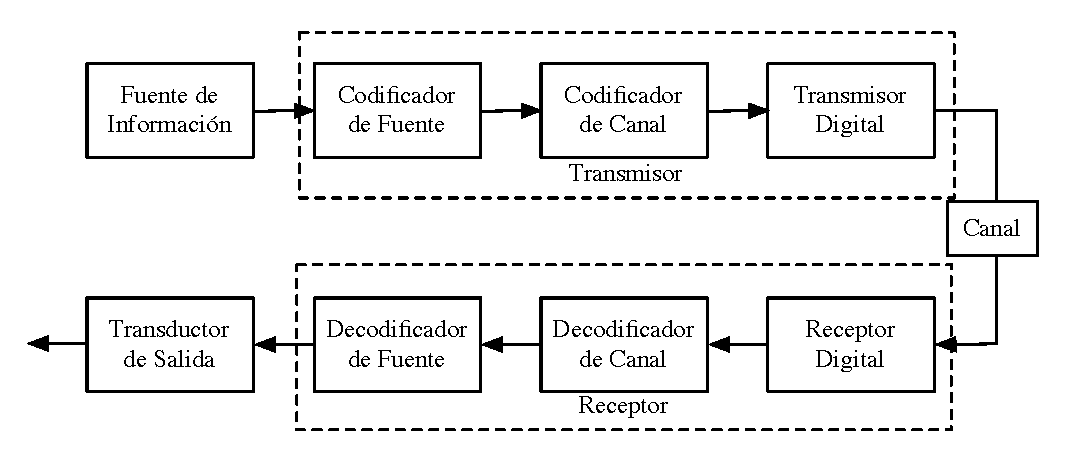
\includegraphics[width=0.95\linewidth]
{introduccion/figuras/fig01-01.pdf}
\caption{Modelo de un sistema de Comunicación Digital I}
\label{fig01-01}
\end{figure}
\end{lstlisting}
%\end{micuadro}

Y el resultado se muestra en la \autoref{fig01-01}.

%
\begin{figure}[htbp]
\centering
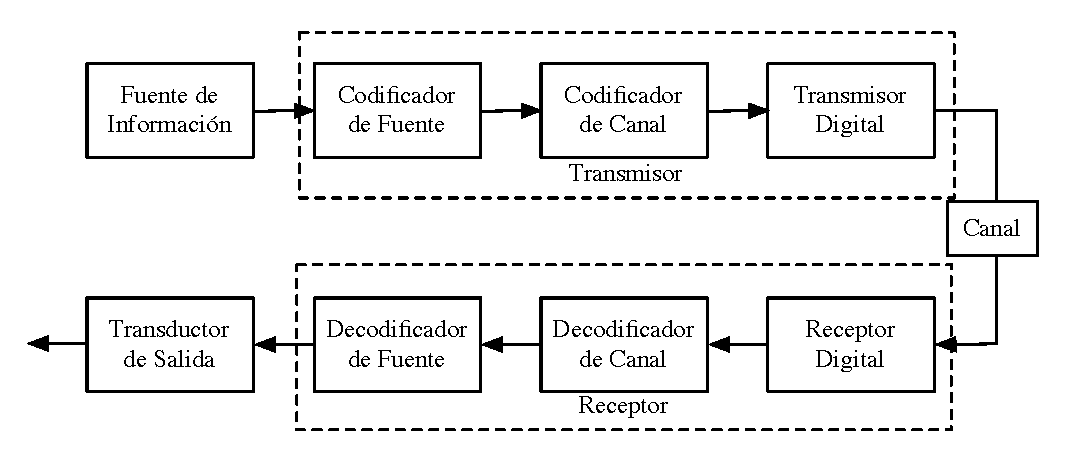
\includegraphics[width=0.95\linewidth]{introduccion/figuras/fig01-01.pdf}
\caption{Modelo de un sistema de Comunicación Digital I}
\label{fig01-01}
\end{figure}
%

Para incluir una tabla utilizamos las instrucciones siguientes:
%\nopagebreak 
\begin{lstlisting}[language=,caption={Inclusión de una tabla}, breaklines=true, label=prg01-02]
\begin{table}[htbp]
	\ttabbox
	{\caption{Tipos de transmisión y frecuencia central} 
	\label{tab2_1}}
		{
		\begin{tabular}{c c}
		\hline
		\rule[-8pt]{0pt}{22pt}{\bfseries{Tipo de Transmisión}}&
		 {\bfseries{Frecuencia central de transmisión}} \\
		\hline
		\rule{0pt}{14pt}Modem & 100-1800 Hz \\
		Radio AM & 530-1600 kHz \\
		Radio FM & 88-108 MHz \\
		Televisión & 178-216 MHz \\
		Telefonía móvil & 850 MHz-1,8 GHz \\
		Redes inalámbricas &  $2,4$ GHz \\
		Fibra óptica & $2\cdot 10^{14}$ Hz \\
		\hline
		\end{tabular}
		}
\end{table}
\end{lstlisting}

Y el resultado se muestra en la \autoref{tab2-1}.

\begin{table}[htbp]
	\ttabbox
	{\caption{Tipos de transmisión y frecuencia central} \label{tab2-1}}
		{
		\begin{tabular}{c c}
		\hline
		\rule[-8pt]{0pt}{22pt}{\bfseries{Tipo de Transmisión}}& {\bfseries{Frecuencia central de transmisión}} \\
		\hline
		\rule{0pt}{14pt}Modem & 100-1800 Hz \\
		Radio AM & 530-1600 kHz \\
		Radio FM & 88-108 MHz \\
		Televisión & 178-216 MHz \\
		Telefonía móvil & 850 MHz-$1,8$ GHz \\
		Redes inalámbricas &  $2,4$ GHz \\
		Fibra óptica & $2\cdot 10^{14}$ Hz \\
		\hline
		\end{tabular}
		}
\end{table}

Observemos  que en la parte inferior de las figuras y en la superior de las tablas (esta ha sido nuestra elección), se colocan textos explicativos sobre las mismas. El formato de este texto se logra mediante una sentencia facilitada por el paquete que se carga mediante el comando \comandos{usepackage}{caption}. El resto de paquetes utilizados realizan diversas tareas como, por ejemplo, \comandos{usepackage}{longtable}, que permite que una tabla se extienda a través de más de una página.

\subsection{Hiperenlaces}
Un primer paso a la hora de crear un documento es generar una versión en formato electrónico del mismo. Hemos decidido que ese formato sea \ttcolor{pdf} . En un formato pdf existe la posibilidad de crear hiperenlaces que facilitan la navegación a lo largo del mismo. Por ejemplo, el índice en un libro en formato pdf se generará, con la propuesta que hemos realizado, creando enlaces a las diversas partes del mismo. O bien, cuando nos referimos a una figura o tabla, es muy útil la existencia de esos enlaces al lugar exacto en el que se encuentra la figura o tabla.  El paquete responsable de realizar todas estas tareas se denomina \ttcolor{hyperref} y las sentencias que siguen a su carga realizan diversas tareas que pueden consultarse en la extensa documentación que lo acompaña. Sobre la línea 110 de \ttcolor{libroTipoETSI.tex} encontrará que puede modificar el color del enlace, puesto a negro por defecto.
% Por ejemplo, no habrá que olvidarse sustituir el literal \ttcolor{F. Javier Payán Somet y Juan José Murillo Fuentes} por el nombre del autor correspondiente.

\subsection{Tabla de contenido}
La generación de la tabla (o tablas) de contenido de un texto suficientemente largo suele ser una tarea sumamente laboriosa. \LaTeX\ facilita enormemente este trabajo mediante un conjunto de paquetes y comandos que se agrupan bajo el apartado genérico denominado TOC (Table Of Contents). En otra sección de este capítulo explicaremos cómo y dónde se incorporará esta tabla de contenidos. En este apartado nos centramos en explicar algunos aspectos de cómo se construye la principal tabla de contenidos, que denominamos  \ttcolor{Índice}.

Nuestra primera decisión fue establecer que en el índice deben aparecer hasta los apartados que hemos denominados \ttcolor{subsubsecciones}, lo que se logra mediante el \ttcolor{\{3\}} del comando \comandos{setcounter}{tocdepth} en \ttcolor{libroETSI.sty}. El formato de cada uno de los apartados se logra con el conjunto de sentencias que siguen y tienen una estructura bastante autoexplicativa. También hemos propuesto que no aparezcan los habituales puntos que existen entre el texto y el número de página correspondiente de muchos índices, ajustando a \ttcolor{10000} el parámetro \ttcolor{\textbackslash@dotsep}. 

Nuestra siguiente decisión afecta a la manera en la que hemos querido que aparezcan en el índice los índices del texto, valga la redundancia. No es trivial pero, básicamente, hemos definido dos listas, una para los elementos que aparecen antes del Índice General y otra para los  que aparecen después, al fina del texto, que se corresponden aproximadamente a lo que hemos denominado \ttcolorc{frontmatter} y \ttcolorc{backmatter}, respectivamente. Si no se desea cualquier índice, basta con comentar la línea correspondiente.

\subsection{Formatos de títulos, páginas y cabeceras y pies de páginas}
El aspecto de un libro está básicamente definido por el formato que se ha elegido para los diferentes títulos de las partes que lo constituyen, el formato de las páginas y qué queremos que aparezca en las cabeceras y pies de páginas del mismo. Todo esto se ha conseguido utilizando un paquete desarrollado por el español Bezos denominado \ttcolor{titlesec}, que se carga en nuestro fichero mediante la instrucción \comandos{usepackage[noindentafter, pagestyles,...]}{titlesec}.

El paquete nos permite definir los distintos tipos de páginas, de acuerdo con las instrucciones que se proporcionan en el mismo. Por ejemplo, con \comandos{newpagestyle}{esitscCD} creamos la página habitual en la mayor parte del texto, formada por el número en la parte exterior de la misma, en las páginas pares el nombre del capítulo en el que estamos y en las impares el nombre de la sección. Estos elementos se colocan encima de una raya horizontal que se ha definido previamente, tanto en su grosor como en su longitud.

Una vez definidos las diferentes tipos de páginas podemos definir, por ejemplo, que nuestra página por defecto será \ttcolor{esitscCD}, con la instrucción \comandos{pagestyle}{esitscCD}. Si queremos que una página determinada en un punto concreto sea diferente, si suponemos que, por ejemplo, el estilo de página \ttcolor{otroestilo} ha sido definido, basta situar la instrucción \comandos{thispagestyle}{otroestilo} en el punto deseado. Un ejemplo podemos encontrarlo en la manera que logramos que los capítulos empiecen siempre en páginas impares. Con ese fin, se utiliza el estilo de página \ttcolor{empty} en caso de que sea necesario.

Por último, el paquete \ttcolor{titlesec} nos permite definir cómo queremos que sean los titulares que usaremos en nuestros textos. Así,  la instrucción \comandos{titleformat}{\textbackslash section ...} establece que nuestras secciones estarán numeradas al nivel de capítulo, con el número de la sección fuera de margen \ttcolor{hang}, y con unas determinadas separaciones del texto, establecidas a través del comando \ttcolorc{titlespacing}. 

En todo caso, estos parámetros no se deberían de tocar, salvo en contadas ocasiones, y por ello se incluyen aquí estos detalles.

\subsection{Teoremas, propiedades, definiciones y demás}
En la escritura de cualquier texto científico los Teoremas, propiedades y demás elementos constituyen una parte muy significativa. Existen, de nuevo, múltiples posibilidades de tratar estos elementos, pero hemos considerado que las facilidades que suministra el paquete \ttcolor{ntheorem}, cargado mediante la instrucción \comandos{usepackage [thmmarks, amsmath, noconfig, hyperref, framed]}{ntheorem} se adapta perfectamente a nuestros gustos y decisiones. Por ejemplo, con el conjunto de instrucciones que se muestran en  el Código \ref{prg01-03}:

\begin{lstlisting}[language=TeX,caption={Teoremas, Lemas,...}, breaklines=true, label=prg01-03]
\theoremnumbering{arabic}
\theoremheaderfont{\aheadteoremas}
\theoremseparator{\hspace{.2em}}
\theorembodyfont{\itshape}
\newtheorem{teor}{Teorema}[section]
\newtheorem{lema}{Lema}[section]
\newtheorem{prop}{Propiedad}[section]
\newtheorem{coro}{Corolario}[teor]
\end{lstlisting}

\noindent hemos definido los Teoremas, Lemas, Propiedades y Corolarios. Centrándonos en los teoremas, las instrucciones anteriores definen que los teoremas estarán referenciados mediante un número \ttcolor{arabic}, con una numeración que será creciente desde la unidad dentro de cada sección de un determinado capítulo, \comandos{newtheorem\{teor\}}{Teorema}\ttcolor{[section]}. La fuente que se utilizará para que aparezca la palabra ``Teorema'' está definida por el comando \ttcolor{\textbackslash theoremheaderfont\{\textbackslash aheadteoremas\}}, el enunciado del teorema se realizará en itálica y para enunciar un teorema y su demostración utilizamos las siguiente instrucciones:

\begin{lstlisting}[language=TeX,caption={Teorema y Demostración}, breaklines=true, label=prg01-04]
\begin{teor}[Teorema de Pitágoras]
En un triángulo rectángulo...
\end{teor}
\begin{proof}
Sea el triángulo ABC...
\end{proof}
\end{lstlisting}

El resultado sería el siguiente:
\begin{teor}[Teorema de Pitágoras]
En un triángulo rectángulo...
\end{teor}
\begin{proof}
Sea el triángulo ABC...
\end{proof}

Podemos observar que al finalizar la demostración hemos incluido el símbolo $\blacksquare$. De manera análoga, están definidas las restantes entidades, incluyendo el comando que nos permite escribir los cuadros de elementos de la programación.

\subsection{Índices de palabras y glosarios}
Con los paquetes index y glossaries podemos incluir índices de palabras y listas con definiciones, ya sea de acrónimos u de otro tipo. Por ejemplo, se podría usar también para definir magnitudes o la notación utilizada.
 
%http://en.wikibooks.org/wiki/LaTeX/Indexing
\subsubsection{Índices de palabras}
\index{Indice de palabras@Índice de palabras!index}%\index{\'Indice de palabras!index}\index{Índice de palabras!indexit}
Para construir un índice de palabras\index{Indice de palabras@Índice de palabras}, como el que puede encontrar al final de este texto, se incluye el paquete \comandos{usepackage}{imakeidx} con algunas opciones. Para incluir una palabra  en el índice utilizamos   \comandos{index}{palabra} justo detrás de la palabra que queramos indexar. Si queremos agrupar en un grupo diferentes subpalabras \index{Indice de palabras@Índice de palabras!subpalabra}, utilizamos \comandos{index}{palabra!subpalabra}. Es importante no olvidar ejecutar \ttcolor{makeindex}, al igual que ejecuta latex o bibtex para componer el texto o generar la bibliografía. Otro detalle importante es poner los índices con mayúsculas o con minúsculas, pero todos iguales. De esta forma, cuando se genere el índice de palabras no queden algunas con la primera letra en mayúsculas y otras no. Por último, con las instrucciones de compilación que se detallan un poco más adelante, las palabras en español que empiecen por tilde se indexan al final. Para evitarlo, y que aparezcan en su sitio, tiene que escribir primero la palabra sin tilde seguida de arroba y la palabra con tilde, como por ejemplo \ttcolorc{index\{Indice de palabras@Índice de palabras\}}. 

\subsubsection{Glosario}
Un glosario con acrónimos u otros términos se realiza en este texto utilizando\\
 \comandos{usepackage [acronym]}{ glossaries}. 
 Para definir un acrónimo, basta con incluir antes del comienzo del documento una línea del tipo:\\
 \comandos{newacronym[type=main]\{etiqueta\}\{acrónimo\}}{nombre completo}, 
 \\
 como por ejemplo\\
 \comandos{newacronym[type=main]\{ETSI\}\{ETSI\}}{Escuela Técnica Superior de \\Ingeniería}. 
 \\
 En esta orden el primer argumento es el identificador o etiqueta, el segundo es el acrónimo o abreviatura y el tercero es el nombre completo al que hace referencia el acrónimo o abreviatura. Para utilizar luego la abreviatura o acrónimo, y se pueda luego generar un índice que indique en qué página se ha usado, se utiliza \comandos{gls}{etiqueta}. 

\subsubsection{Compilación de índices de palabras y glosarios}
Existen distintos comandos para generar el índice y el glosario. Puede utilizar los que estime oportunos. Aquí se ofrece una solución para realizarlo.

El comando más usado es \ttcolor{makeindex}. Habría que llamar dos veces a este comando, con distintos argumentos, si se incluye el glosario además del índice. En Macintosh si utiliza el comando \ttcolor{lualatexmk}, uno de los engines de TeXShop\index{engine}, el índice de palabra y el glosario se generarán de forma automática. 
%Puede usar Texindy\index{Texindy} para una presentación del índice de palabras con otra presentación.

En Windows, tendrá que ejecutar PDFLatTeX ó LatexMk, luego tendrá que ejecutar makeindex tal cual para generar el índice de palabras. Para generar el glosario tendrá que definir un comando de usuario, tal como sigue. Vaya al menú `Usuario', en texmaker, y allí a `Comandos de Usuario' y dentro de este a `Editar Comandos de Usuario'. En cualquiera de los comandos defina uno nuevo con el título que quiera, por ejemplo glosario, y en el campo comando, incluya la siguiente línea\footnote{Si usase el texmaker en Mac-OS tendría que pulsar el asistente para seleccionar makeindex. Aparecería en el campo comando algo así como \ttcolor{''makeindex'' \%.idx}, donde el asistente habrá encontrado la carpeta donde está el comando makeindex. Sustituya el final, \%idx, por  -s \%.ist -t \%.glg -o \%.gls \%.glo, de forma que el campo comando quede como sigue:
 \ttcolor{''/usr/texbin/makeindex'' -s \%.ist -t \%.glg -o \%.gls \%.glo}}

Una vez definido este comando de usuario, ejecútelo, y vuelva a ejecutar PDFLaTeX o LatexMk.

\section{Antes del documento}
Antes de empezar la edición del documento, además de cargar los ficheros de estilos \ttcolor{LibroETSI.sty} y \ttcolor{edicionLibro.sty} (o el correspondiente al documento),  hemos creído necesario realizar una serie de operaciones que faciliten nuestro trabajo o lo configuren de una determinada manera. %Además, hay que incluir la portada.

\subsection{Fichero de notación: notacion.sty}
Hemos considerado interesante incluir un fichero de notaciones que son de amplia utilidad dentro del área de conocimiento de los autores. Su uso es completamente opcional pero se ha utilizado ampliamente en la elaboración de este texto. Simplifica enormemente la escritura hacer uso de ficheros de este tipo y prácticamente cada autor utiliza el suyo propio.

Como ocurría con el fichero \ttcolor{LibroETSI.sty}, es necesario que se cargue, incluyendo la instrucción \comandos{usepackage}{notacion} al comienzo del fichero principal. Puesto que su uso resulta evidente, no hemos considerado necesario realizar una documentación precisa sobre el mismo más allá de los propios comentarios que acompañan las definiciones del fichero, y que el lector puede consultar abriéndolo. Nótese que existe además una carpeta con este nombre. En esta carpeta se ha incluido un ejemplo de notación que podría ponerse al comienzo de un documento. Sobre este documento, se puede añadir o quitar lo que se desee.

\subsection{Fuente del texto}
Las instrucciones incluidas en el código \ref{prg01-05} y que pertenecen al fichero \ttcolor{LibroETSI.sty} 
 se pueden modificar para cambiar la fuente del texto.  En primer lugar, debemos actuar de forma diferente si queremos utilizar la fuente Minion Pro o no.  Si hemos definido como \ttcolor{true} el parámetro correspondiente, en el caso que estemos compilando con \LaTeX\ no debemos hacer nada. Sin embargo, en el caso de utilizar \LuaLaTeX\ debemos declarar que la fuente va a ser Minion Pro y modificar ligeramente su tamaño.
 
Si no vamos a utilizar una fuente Minion Pro, en el caso de \LuaLaTeX\ se puede utilizar para el texto cualquier fuente OTF o TTF que el usuario posea de forma legal, y se encuentre instalada, lo que depende del sistema operativo (SO) utilizado. En nuestro caso, observad que hemos utilizado una fuente Time New Roman  pues suele estar instalada en la mayoría de los SO. Se proponen asimismo un par de alternativas si prefiere otras fuentes.
 
El código incluido detecta si se no se está utilizando \LuaLaTeX\, en cuyo caso se usa una fuente equivalente a una Times, cargada mediante el comando estándar \comandos{usepackage}{tgtermes}. Hay otras opciones comentadas, y se pueden buscar otras fuentes. 
 
\begin{lstlisting}[language=,caption={Fuente del texto}, breaklines=true, label=prg01-05]
%:Para modificar fácilmente la fuente del texto. 
\makeatletter
\ifdtsc@Minion % Queremos utilizar la fuente Minion y lo hemos declarado al principio
	\ifluatex
		\setmainfont[Renderer=Basic, Ligatures=TeX,	% Fuente del texto 
		Scale=1.01,
		]{Minion Pro}
   		% En este caso conviene modificar ligeramente el tamaño de las fuentes matemáticas
		\DeclareMathSizes{10}{10.5}{7.35}{5.25}
		\DeclareMathSizes{10.95}{11.55}{8.08}{5.77}
		\DeclareMathSizes{12}{12.6}{8.82}{6.3}
	\fi
\else
	\ifluatex
		% Para utilizar la fuente Times New Roman, o alguna otra que se tenga instalada
		\setmainfont[Renderer=Basic, Ligatures=TeX,	% Fuente del texto 
		Scale=1.0,
		]{Times New Roman}
%		\setmainfont[Renderer=Basic, Ligatures=TeX,	% Fuente del texto 
%		]{Adobe Garamond Pro}
%		\setmainfont[Renderer=Basic, Ligatures=TeX,	% Fuente del texto 
%		]{Palatino LT Std}
	\else
		\usepackage{tgtermes} 	%clone of Times
		%\usepackage[default]{droidserif}
		%\usepackage{anttor} 	
	\fi
\fi
\makeatother
\end{lstlisting}

Si se intenta utilizar una fuente que no está instalada (dentro del sistema operativo) la compilación con \LuaLaTeX\ daría error. Si se instala una nueva fuente y se desea utilizar, se puede tratar de modificar las líneas de código que se suministran como ejemplo. La primera vez que se utilice esa nueva fuente, \LuaLaTeX\ tardará algo más en compilar pues necesita generar una serie de ficheros internos.

La principal ventaja en el uso de \LuaLaTeX\ la encontramos en la facilidad para utilizar diferentes fuentes en diferentes lugares y con diferentes características (tamaño, color, etc) muy fácilmente configurables. Puede ser interesante leer el fichero \ttcolor{fontspec.pdf} para conocer cómo se realizan estos cambios. 

En caso de utilizar el motor pdfLatex, la elección más sencilla se realiza como hemos dicho mediante paquetes específicos tales como \comandos{usepackage}{tgtermes}. Puede consultarse la dirección \url{http://www.tug.dk/FontCatalogue/alphfonts.html} para conocer las posibilidades más habituales. 

Por último: como ya hemos dicho, todo lo anterior únicamente afecta a la elección de las fuentes del texto. La elección de las fuentes matemáticas (texto dentro de matemática, símbolos, letras griegas, etc) se controla de manera completamente diferente mediante paquetes específicos. En el \autoref{estilo} volveremos sobre este asunto. En concreto, observar que en el caso de compilar con la opción \ttcolor{Minion=true} y existir el fichero de estilo \ttcolor{MinionPro.sty} (no confundir con la fuente Minion Pro; si no existiera el fichero, aparecería un error), se propone el uso de la fuente Minion Pro como fuente matemática, junto con los símbolos de la fuente MnSymbol. En caso contrario, se hará uso de una fuente Times (en realidad, de una extensión de la misma). 

No todas las fuentes pueden usarse como fuentes matemáticas y en la dirección \url{http://www.tug.dk/FontCatalogue/alphfonts.html} se encuentran recogidas las que si tienen soporte matemático. Es importante señalar además que no todas las combinaciones de fuente de texto y fuente matemática son tipográficamente adecuadas. 

\subsection{Cubierta y primeras páginas}
Se ha diseñado esta plantilla para que tome una imagen de fondo y a partir de ésta se incluyan los datos de título, autor, etc, para generar la portada del documento. La portada propuesta es distinta para proyectos fin de carrera y similares que para libros o tesis. Todo esto se ha hecho diseñando una serie de funciones que las generan, tomando los datos que se definen en la cabecera del fichero principal. Así, en el \ttcolor{libroTipoETSI.tex}, se puede definir el título de la obra, el autor, etc. En el caso de \ttcolor{pfcTipoETSI.tex} y \ttcolor{tesisTipoETSI.tex}, se puede definir además el director, el tipo de proyecto (máster, grado y carrera), y otros parámetros. Las imágenes de fondo de la cubierta también se llaman desde este fichero, así como la imagen al pié de la hoja interior con el título y autor de la obra (para libros). La imagen central de la cubierta está en la carpeta figuras, con nombre \ttcolor{imagenLibro.png}. Puede incluir la imagen deseada en esta carpeta salvándola con este mismo nombre. Preste atención a que el formato es rectangular. Para introducir la imagen del logo del departamento en el proyecto fin de carrera/grado/máster, puede retocar la imagen de fondo, cortando el logo existente e insertando el deseado. Estas imágenes están en la carpeta figuras. 

Para cambiar cualquier otro aspecto, tales como el tamaño de la figura de la cubierta ó los créditos de la cubierta, tendrá que modificar el fichero \ttcolor{edicionLibro.sty} en este caso de un libro. 

%En el ejemplo que se presenta para libros, el latex toma una imagen de fondo, y otra, imagenLibro.png,  de la portada para incluir además de los datos de título y autores, definidos al comienzo del fichero \ttcolor{portadaLibro.tex}, una imagen superpuesta representativa de la temática del texto. Los autores pueden cambiar esta imagen fácilmente por otra acorde a su texto.

%Sería interesante poner algo sobre citas

\endinput


% !TEX root =../LibroTipoETSI.tex
\chapter{Ejemplo de Capítulo}\LABCHAP{CAPEJ}
\pagestyle{esitscCD}
\epigraph{ Una de las virtudes del ingeniero es la eficiencia.  }{Guang Tse}

%\lettrine[lraise=0.7, lines=1, loversize=-0.25]{E}{l} 
\lettrine[lraise=-0.1, lines=2, loversize=0.25]{E}l \emph{formato de capítulo }\index{formato!de capítulo} abarca diversos factores. Un capítulo puede incluir, además de texto, los siguientes elementos:
%http://en.wikibooks.org/wiki/LaTeX/List_Structures#Customizing_Lists

\begin{itemize}\itemsep1pt \parskip0pt \parsep0pt
\item \indexit{Figuras}
\item \indexit{Tablas}
\item \indexit{Ecuaciones}
\item \indexit{Ejemplos}
\item \indexit{Resúmenes}, con recuadros en gris, por ejemplo
\item \indexit{Lemas}, \indexit{corolarios}, \indexit{teoremas},... y sus demostraciones
\item \indexit{Cuestiones}
\item \indexit{Problemas} propuestos
\item ...
\end{itemize}

En este capítulo se propone incluir ejemplos de todos estos elementos, para que el usuario pueda modificarlos fácilmente para su uso. Consulte el código suministrado, para ver cómo se escriben en \LaTeX.

\section{Ejemplo de sección}\LABSEC{SEC}
%
En la \FIG{FIG} se incluye a modo de ejemplo la imagen del logo de la \gls{ETSI} \footnote{Se usa aquí el package de acrónimos, que la primera vez define el acrónimo y ya luego sólo incluye el mismo. Esto facilita luego generar de forma automática la lista de acrónimos.}. El código para que aparezca dicha imagen se muestra en el cuadro siguiente:



Si nos detenemos en los comandos que hemos utilizado, con \ttcolor{width} se controla el ancho, y se escala así el tamaño de la imagen. En \LaTeX existen diversas opciones para situar la figura en la página: con \ttcolor{t} o \ttcolor{b} se le indica que las incluya arriba o abajo (top/bottom) y con \ttcolor{!} se le pide que la deje dónde está, tras el texto anterior.


\begin{lstlisting}[language=TeX,caption={Código para incluir una figura}, breaklines=true, label=prg01-01]
\begin{figure}[htbp]
\centering

\includegraphics[width=3 cm]{capituloLibroETSI/figuras/logoESI.pdf}
\caption{Logo de la ETSI}
\label{fig:figura1}
\end{figure}
\end{lstlisting}


\begin{figure}[htbp]
\centering
%
\includegraphics[width=0.2\linewidth]{capituloLibroETSI/figuras/logoESI.pdf}

\includegraphics[width=3 cm]{capituloLibroETSI/figuras/logoESI.pdf}
\caption{Logo de la ETSI}
\LABFIG{FIG} %Esto es una forma propia de los autores de gestionar las etiquetas y referencias
\end{figure}
%

Para dar énfasis a algún texto, usamos \ttcolorc{emph}. %Este comando es de los denominados \emph{inteligentes} apareciendo el texto \emph{resaltado} dependiendo del contexto.  
Así, por ejemplo, 
\begin{caja}
\emph{No olvide intentar utilizar este formato en sus publicaciones de la \gls{ETSI}}
\end{caja}
hace aparecer el anterior texto en itálica. Pero si escribiésemos, por ejemplo, 
\begin{caja}
\emph{No olvide intentar utilizar este formato \emph{siempre} en sus publicaciones de la \gls{ETSI}}
\end{caja}
vemos cómo hemos destacado la palabra ``siempre'' en torno a su contexto. Para ello, hemos escrito, realmente, \comandos{emph}{siempre} dentro de la frase original.
%
\subsection{Ejemplo de subsección}\LABSSEC{EjSS}
%
Si se usaba \ttcolorc{section} para indicar una sección, se utiliza \ttcolorc{subsection} para una subsección.


\section{Elementos del texto}
%

\subsection{Figuras}

Además del tipo de figura que vimos anteriormente, el normal, podemos desear incluir una figura en modo apaisado ocupando toda la página. Para ello utilizamos el entorno de figura siguiente \comandos{begin}{sidewaysfigure}, cuyo resultado se puede observar en la \FIG{FigApaisada}. 

\begin{sidewaysfigure}
\centering
%
\includegraphics[width=0.2\linewidth]{capituloLibroETSI/figuras/logoESI.pdf}

\includegraphics[width=3 cm]{capituloLibroETSI/figuras/logoESI.pdf}
\caption{Logo de la ETSI}
\LABFIG{FigApaisada}
\end{sidewaysfigure}

Aunque puede optar por la forma que desee, en el fichero \ttcolor{notacion.sty} se incluyen definiciones para que pueda usar \comandos{LABFIG}{etiqueta} y \comandos{FIG}{etiqueta} para poner una etiqueta y hacer referencia a la misma luego. Además, está definido para que \comandos{FIG}{etiqueta} incluya por delante el término Figura.

\subsection{Tablas}
A modo de ejemplo, \TAB{Tab1} incluye un ejemplo de tabla. Al igual que con figura, si usa \ttcolor{notacion.sty} puede usar \comandos{LABTAB}{etiqueta} y \comandos{TAB}{etiqueta} para poner una etiqueta y una referencia, y el \comandos{TAB}{etiqueta} ya incluye el nombre Tabla por delante.

Una alternativa al uso de estos comandos está representado por el uso del comando \ttcolorc{autoref\{etiqueta\}} que, en conjunción con el paquete \ttcolor{babel} genera automáticamente los nombres de Figura o Tabla, en función de la etiqueta correspondiente.

\begin{table}[h]
%\small
\caption{Valores de parámetros}
\begin{center}
\begin{tabular}{p{7cm}p{2cm}p{2cm}} %Con esto definimos el ancho de cada columna
Definición & notación & valor\\
 \hline
Potencia transmitida	(entregada a antena) & $P_{et}$ & -5 a 20 dBm	\\
Ganancia antenas & $G$ & $40.5$ dBi\\	
 \hline
\end{tabular}
\end{center}
\LABTAB{Tab1}
\end{table}%

\subsection{Listados de programas}
Es muy habitual en nuestros documentos que tengamos que incluir listados de programas. Para ello, se propone la utilización de un paquete denominado \ttcolor{listings}. Se obtiene con él un listado como el mostrado en el \autoref{prg02-01} de \matlab siguiente: 

\begin{lstlisting}[language=Matlab,caption={Representación de la función $\rect(t-T/2)$}, breaklines=true, label=prg02-01]
clear all
close all
T = 1;
A = 1;
L = 100;
tstep = T/L;                                
t = 0:tstep:T-tstep;   
g_t = A*ones(1,L); 
figure(1);
subplot(211);
h=plot(t,g_t); axis( [0 T -A-0.1 A+0.1]);
set(h,'linewidth', 1.0);
ylabel('g(t)'), xlabel('t[s]'); grid on;

g_n = g_t;
subplot(212);
h=stem(g_n, '.', 'filled'); axis( [1 L -0.1 A+0.1]);
set(h,'linewidth', 1.0);
ylabel('g(n)'), xlabel('n');
\end{lstlisting}

También se puede generar en este caso una relación de los códigos usados en nuestro documento, de manera equivalente a la relación de figuras o tablas. Para ello, observar la correspondiente codificación en el fichero principal.
 
\subsection{Ecuaciones}%%%%%%%%%%%%%%%%%%%%%%%%%%%%%%%%%%%%%%%
Para escribir expresiones matemáticas, como por ejemplo $2+2=4$, sólo hace falta que meta la expresión entre símbolos \ttcolor{\$}. En el fichero notacion.sty se incluyen muchas definiciones para facilitar la escritura de estas expresiones y de ecuaciones. Para escribir una ecuación, con una o más líneas, se aconseja utilizar \ttcolor{align}, como en el siguiente ejemplo, en las ecuaciones \EQ{Eq1}-\EQ{Eq3},
\begin{align}
 T     &=kT_b  \LABEQ{Eq1}, \\
 R_b&=\frac{1}{T_b }	, \\
 D    &=\frac{1}{T}=\frac{R_b }{k}=\frac{R_b}{\log_2 M}. \LABEQ{Eq3}
\end{align}
Si no quiere numerar una línea, utilice las instrucción \comando{nonumber} antes de poner \verb+\\+  para escribir la siguiente línea. Y con \& puede alinear las ecuaciones. 

Un ejemplo más complejo de ecuaciones sería el siguiente: decimos que el vector aleatorio $\vc{Z}$ es gaussiano si su función densidad de probabilidad conjunta viene dada por:
\begin{equation}\label{eq02-x131}
f_{\vc{Z}}\left( {\vc{z}} \right)= \frac{1}{\left( {2\pi} \right)^{N}{\left| {\vc{C_{Z}}} \right|}^{1/2}}\e^{-\frac{1}{2}\left( {\vc{z}-\vc{m_{Z}}} \right)\trs\vc{C_{Z}}^{-1}\left( {\vc{z}-\vc{m_{Z}}} \right) }
\end{equation}
con el vector media la matriz $\vc{m_{Z}}$ y la matriz de covarianza real $\vc{C_{Z}}$ $\left( {2N \times 2N} \right)$ simétrica definida positiva dado por:
\begin{equation}\label{eq02-x132}
\vc{m_{Z}}=\begin{bmatrix}
\vc{m_{X}}\\
\vc{m_{Y}}
\end{bmatrix}, \quad
\vc{C_{Z}}=\begin{bmatrix}
\vc{C_{X\hphantom{X}}} & \vc{C}_\vc{XY}\\
\vc{C_{YX}} & \vc{C_{Y\hphantom{X}}}
\end{bmatrix}
\end{equation}

con el vector $\bm{\omega}$ dado por:
\begin{equation}\label{eq02-y410}
\bm{\omega}=\begin{bmatrix}
\omega_{1}\\
\vdots \\
\omega_{N}\\
\omega_{N+1}\\
\vdots \\
\omega_{2N}
\end{bmatrix}
\end{equation}
Si no desea que se numere una ecuación puede poner asterisco, tanto en el entorno \verb+equation+ como \verb+align+.


\subsection{Ejemplos}%%%%%%%%%%%%%%%%%%%%%%%%%%%%%%%%%%%%%%%

Para incluir un ejemplo, utilize el entorno \comando{ejmp}, usando el entorno \comando{begin\{ejmp\}} y \comando{end\{ejmp\}}, y para la solución el entorno  \comando{begin\{sol\}}. 

\begin{ejmp}
Calcule $2+2$.
\end{ejmp}
\begin{sol}
%
Para resolver esto se puede utilizar que $1+1=2$, de la siguiente forma
\begin{equation*}% con el * se evita que se numere la ecuación
2+2=(1+1)+(1+1)=4,
\end{equation*}
donde se ha contado, pruebe a utilizar los dedos de su mano, a cuatro.
\end{sol}

Observad que antes de comenzar el ejemplo y tras su finalización se han incluido unos \emph{filetes} a modo de resalte en el texto. En el caso de una serie de ejemplos, los entornos \comando{begin\{ejmpn\}} y  \comando{begin\{soln\}}, junto con los entornos de cierre correspondientes, permiten que no existan estos filetes entre los ejemplos y soluciones intermedias de la serie.
 
\subsection{Lemas, teoremas y similares}

Se incluyen ejemplos de estos elementos de texto. Empezamos con la \DFN{D11} y la \PRP{P11}:

\begin{defn}[Suma]\LABDFN{D11}
 La suma es la operación que permite contar sobre un número, otro.
\end{defn}


\begin{prop}[Suma]\LABPRP{P11}
 Los números enteros se pueden sumar.
\end{prop}


\begin{lema}[Suma de 1 y 1]\LABLEM{L11}
 La suma $1+1$ es igual a $2$.
\end{lema}
\begin{proof}
Ponga un dedo a la vista, junto a otro, y cuéntelos.
\end{proof}


\begin{teor}[Suma]\LABTHM{T11}
 La suma de cualquier número y dos es igual a la suma del mismo número más uno más uno.
\end{teor}
\begin{proof}
Por inducción y el \LEM{L11}.
\end{proof}

\begin{coro}[Contables]\LABCOR{C11}
  Los números enteros son contables.
\end{coro}
\begin{proof}
Por el \THM{T11}.
\end{proof}


\subsection{Resúmenes}%%%%%%%%%%%%%%%%%%%%%%%%%%%%%%%%%%%%%%%
Para incluir un resumen de una sección o un conjunto de secciones o en cualquier otro punto que consideremos interesante, se utiliza el entorno \comando{begin\{Resumen\}}, que admite como parámetro opcional un nombre que queramos asignarle al resumen. Por defecto, se denomina ``Resumen''. Observar que se ha modificado la cabecera de las páginas impares. Una vez finalizado el resumen, con el comando \comando{end\{Resumen\}}, se recupera la anterior cabecera automáticamente. Los resúmenes que se deseen incluir aparecen en la tabla de contenidos como una sección sin numeración, con el nombre elegido o el nombre por defecto de Resumen. En el siguiente ejemplo hemos utilizado este parámetro opcional de nombre.

\begin{Resumen}[Resumen de Teoría de Información]
\noindent Debido al considerable número de definiciones, teoremas y propiedades que hemos descrito en los apartados anteriores, vamos a presentar un resumen de los principales resultados, no necesariamente en el mismo orden que el expuesto anteriormente. Supondremos en este resumen que las variables aleatorias $X$,  $Y$ y $Z$ son discretas, definidas en el alfabeto $\calg{X}$, $\calg{Y}$  y  $\calg{Z}$ respectivamente. 

\subsubsection*{Entropía de una variable aleatoria discreta}
Se define la entropía $H\left( {X} \right)$ de una variable aleatoria discreta $X$ , con función masa de probabilidad $p\left( {x} \right)$, en la forma:
\begin{equation*}
H\left( {X} \right)= -\sum_{x\in \calg{X} }{p\left( {x} \right)\log p\left( {x} \right)}=\E\left[ -{\log p\left( {X} \right)} \right]
\end{equation*}
\begin{enumerate}
\item Se cumple:
\begin{equation*}
 0\le H\left( {X} \right) \le \log \card{\calg{X}}
\end{equation*}
 con la igualdad en la izquierda si y sólo si $p\xb{i}=1$ para algún $x_{i} \in \calg{X}$ y con la igualdad a la derecha si y sólo si la variable aleatoria está uniformemente distribuida; esto es, $p\xb{i}=1/\card{\calg{X}} \; \mbox{para todo }i$.
 \item $H\left( {X} \right)=0$ si y sólo si $X$ es determinista.
\item $H\left( {X} \right)=H\left( {p\left( {x} \right)} \right)$ es una función cóncava en $p\left( {x} \right)$.
\item Se define la \emph{Función de Entropía Binaria} en la forma:
\begin{equation*}
h_{b}\left( {p} \right) \eqdef -p\log p-\left( {1-p} \right)\log\left( {1-p} \right)\end{equation*}
\item La función entropía binaria $h_{b}\left( {p} \right)$ es una función cóncava en $p$.
\item Si $X$ y $\hat X$ son dos variables aleatorias estadísticamente independientes igualmente distribuidas, 
\begin{equation*}
\Pr\left( {X=\hat X} \right) \ge 2^{-H\left( {X} \right)}
\end{equation*}
con la igualdad si y sólo si $X$ tiene una distribución uniforme.
\end{enumerate}

\subsubsection*{Entropía conjunta y entropía condicional}
Definimos la \emph{entropía conjunta} de las variables aleatorias $X$ e $Y$, $H\left( {X,Y} \right)$ en la forma:
\begin{equation*}
H\left( {X,Y} \right)=\sum_{x\in \calg{X} }{\sum_{y\in \calg{Y}}{p\left( {x,y} \right)\log \frac{1}{p\left( {x,y} \right)}}}=\E\left[ {-\log p\left( {X,Y} \right)} \right]
\end{equation*}

Definimos la \emph{entropía condicional} $H\left( {X \mid Y} \right)$ en la forma:
\begin{align*}
H\left( {X \mid Y} \right)&=\sum_{y\in \calg{Y}}{p\left( {y} \right)H\left( {X \mid Y= y} \right)}=  \\
&=-\sum_{x\in \calg{X}}{\sum_{y\in \calg{Y}}{p\left( {x,y} \right) \log p\left( {x \mid  y} \right)}}= \\
&=\E\left[ {-\log p\left( {X\mid Y} \right)} \right]
\end{align*}

\begin{enumerate}
\itemv[10]
\begin{equation*}
H\left( {X,Y} \right) \le H\left( {X} \right)+ H\left( {Y} \right)
\end{equation*}
con la igualdad si y sólo si $X$ e $Y$ son estadísticamente independientes.
\itemv[10]
\begin{align*}
H\left( {X\mid Y} \right) &\le H\left( {X} \right) \\
H\left( {Y\mid X} \right) &\le H\left( {Y} \right)
\end{align*}
con la igualdad si y sólo si $X$ e $Y$ son estadísticamente independientes.
\item $H\left( {X\mid Y} \right)=0$ si y sólo si $X$ es una función de $Y$.
\itemv[10]
\begin{equation*}
H\left( {X \mid X} \right) =0
\end{equation*}
\itemv[10] 
\begin{equation*}
H\left( {X,Y} \right)=H\left( {Y} \right)+H\left( {X\mid Y} \right)
\end{equation*}
\itemv[10] 
\begin{equation*}
H\left( {X,Y} \right)=H\left( {X} \right)+H\left( {Y\mid X} \right)
\end{equation*}
\itemv[10] 
\begin{equation*}
H\left( {X,Y \mid Z} \right)=H\left( {X\mid Z} \right)+H\left( {Y\mid X,Z} \right)
\end{equation*}
\item \emph{Desigualdad de Fano} Sean $X$ y $\hat{X}$ dos variables aleatorias que toman valores en el mismo alfabeto \calg{X}. Se verifica:
\begin{equation*}
H\left( {X\mid \hat{X}} \right) \le h_{b}\left( {p\xb{e}} \right)+p\xb{e}\log \left( {\card{\calg{X}}-1} \right)
\end{equation*}
\end{enumerate}
%
\subsubsection*{Reglas de las cadenas}
Sea $\mathbf{X}$   un vector formado por las $N$ variables aleatorias $X_{i}, i=1, 2, \ldots,N$.
\begin{enumerate}
\item \emph{Regla de la cadena para la entropía}
\begin{align*}
H\left( {X_{1}, X_{2}, \ldots, X_{N}} \right)&=\sum_{i=1}^{N}{H\left( {X_{i}\mid X_{1},\ldots, X_{i-1}} \right)}= \\
&=H\left( {X_{1}} \right)+H\left( {X_{2}\mid X_{1}} \right)+ \cdots +H\left( {X_{N}\mid X_{1},\ldots, X_{N-1}} \right) 
\end{align*}
\item \emph{Regla de la cadena para la entropía condicional}
\begin{equation*}
H\left( {X_{1}, X_{2}, \ldots, X_{N} \mid Y} \right)=\sum_{i=1}^{N}{H\left( {X_{i}\mid X_{1},\ldots ,X_{i-1}, Y} \right)}
\end{equation*}
\item \emph{Regla de la cadena para la información mutua}
\begin{equation*}
I\left( {X_{1}, X_{2}, \ldots, X_{N} ; Y} \right)=\sum_{i=1}^{N}{I\left( {X_{i} ;Y \mid X_{1},\ldots, X_{i-1}} \right)}
\end{equation*}
\item \emph{Regla de la cadena para la Información Mutua Condicional}
\begin{equation*}
I\left( {X_{1}, X_{2}, \ldots, X_{N} ; Z \mid Y} \right)=\sum_{i=1}^{N}{I\left( {X_{i} ;Z \mid X_{1},\ldots, X_{i-1},Y} \right)}
\end{equation*}
\end{enumerate}
\end{Resumen}

\section{Una nueva sección después del resumen}


%%%%%%%%%%%%%%%%%%%%%%%%%%%
%%%%%%%%%%														
%%%%%%%%%%					Problemas							
%%%%%%%%%%														
%%%%%%%%%%%%%%%%%%%%%%%%%%%


\cleardoublepage
\subchapter{Problemas Propuestos}
\setenumerate[1]{label=\bfseries{\alph*)\quad}, labelindent=\parindent}
\setenumerate[2]{label=\bfseries\arabic*.}
\setenumerate[3]{label=\bfseries{\roman*})}
\pagestyle{probprop}
\captionsetup[figure]{textformat=simple}

\noindent Esto es un ejemplo de cómo incluir cuestiones y/o problemas al final de un capítulo, con o sin solución. Para poner un problema o cuestión, usar  \comando{begin\{prob\}} y \comando{end\{prob\}}. Para incluir la solución, a continuación usar \comando{begin\{soln\}} seguido del texto terminado en \comando{end\{soln\}}.

% P02-01
\begin{prob}
Sean $A$, $B$ y $C$ sucesos de un cierto experimento con probabilidades dadas por:
\begin{align*}
\Pr\left( {A} \right)=&\frac{1}{3}\\
\Pr\left( {B} \right)=&\frac{1}{4}\\
\Pr\left( {C} \right)=&\frac{1}{5}\\
\Pr\left( {A\cap B} \right)=&\frac{1}{12}\\
\Pr\left( {A\cap C} \right)=&\frac{1}{15}\\
\Pr\left( {B\cap C} \right)=&\frac{1}{20}\\
\Pr\left( {A\cap B\cap C} \right)=&\frac{1}{30}
\end{align*}
\begin{enumerate}
\item ¿Son los sucesos independientes dos a dos? ¿Son estadísticamente independientes?
\item Encontrar $\Pr\left( {A\cup B} \right)$.
\item Encontrar $\Pr\left( {A\cup B\cup C} \right)$.
\end{enumerate}
\end{prob}

\begin{prob}
Suponer que tenemos una moneda con las siguientes características: cuando se lanza, la probabilidad de que salga cara es  $\Pr\left( {c} \right)=p$ y la probabilidad de que salga cruz $\Pr\left( {+} \right)=q$. Lanzamos dos veces la moneda y queremos conocer acerca de la independencia estadísticade los siguientes sucesos:
\begin{align*}
A& = \textrm{Sale c en la primera tirada}\\
B& = \textrm{En las dos tiradas sale lo mismo}\\
C& = \textrm{Sale c en la segunda tirada}
\end{align*}
\end{prob}

\begin{prob}
Determinar la media, la autocorrelación y el espectro densidad de potencia de la salida de un sistema con respuesta impulsiva dada por:
\begin{equation*}
h(n) = \begin{cases}
1 &n=0,2 \\
-2 &n=1  \\
0 & \text{en cualquier otro caso} \\
\end{cases}
\end{equation*}
cuando la señal de entrada es un ruido blanco $X(n)$ con varianza 
$\sigma_X^2$.
\end{prob}

\begin{soln}
Si el ruido es blanco, su valor esperado será cero y su espectro densidad de potencia será una constante: $S_{X}\left( {\Omega} \right)=C$. Calculemos su autocorrelación. Se tiene:
\begin{align*}
 R_X (k)&=\L[F]\ ^{-1}\left[ {S_X \left( \Omega \right)} 
\right]=\L[F]\ ^{-1}\left[ C \right]=\frac{1}{2\pi }\int_{-\pi }^\pi 
{Ce^{jk\Omega }\mathrm{d}\Omega } =
\begin{cases}
   {k\ne 0}	   &  \frac{C}{2\pi }\left. {\frac{\e^{jk\Omega }}{jk}} \right|_{-\pi }^\pi\\
     k=0 & C \\
\end{cases}
\;\Rightarrow \\ 
 R_X (k)&=C\delta(k)=
 \begin{cases}
      C & k= 0\\
      0 & k \ne 0
\end{cases}
 \end{align*}

Ahora bien:  (...)
\end{soln}



%%%%%%%%%%%%%%%%%%%%%%%%%%%%%%%%%%%%%%%
%:Material suplementario

%%%%%%%%%%%%%%%%%%%%%%%%%%%%%%%%%%%%%%%

%%%%%%%%%%%%%%%%%%%%%%%%%%%%%%%%%%%%%%%
\subchapter{Anexo}
\pagestyle{esitscCD}
%

\epigraph{Si quiere introducir un separador dentro de un capítulo puede utilizar la instrucción subchapter. Esto le puede interesar, por ejemplo, para introducir alguna información adicional al final de un capítulo como un anexo al mismo.}


%\noindent 
\lettrine[lraise=-0.1, lines=2, loversize=0.25]{E}{n} las secciones que siguen vamos a repasar algunas materias que utilizamos ampliamente a lo largo del texto y que sostienen de forma rigurosa el estudio de las comunicaciones digitales.

\section{Señales: definición y clasificación}
%
Una \index{señal} puede definirse como una función que transmite información generalmente sobre el estado o el comportamiento de un sistema físico, \cite{oppenheim}. Aunque las señales puedan representarse de muchas maneras, en todos los casos la información está contenida en la variación de alguna magnitud física. Matemáticamente se representan como una función de una  o más variables independientes. Por ejemplo, una señal de voz se puede representar como una función del tiempo y una imagen fotográfica puede representarse como una variación de la luminosidad respecto a dos parámetros espaciales. En cualquier caso, es una práctica común denotar como tiempo, $t$, a la variable independiente, en el caso de una variación continua de la variable independiente, y $n$ en caso contrario.
%
\subsection{Clasificación de señales}%
Establezcamos a continuación una clasificación de las señales atendiendo a diversos puntos de vista.
%
\subsubsection*{Señales deterministas y aleatorias}
%
\index{señal!determinista}\index{señal!aleatoria} %% Índice
Una señal se clasifica como determinista cuando no hay incertidumbre alguna acerca del valor que tiene en cualquier instante de tiempo. Estas señales pueden modelarse como una función matemática, por ejemplo, $g\left( {t} \right) = 10 \cos\left( {4\pi t^{2}} \right)$. 

Una señal aleatoria es aquella para la que existe cierta incertidumbre respecto a su valor. Matemáticamente vamos a modelarla como una función muestra de un proceso aleatorio.

Para que una señal transmita información debe tener un carácter aleatorio, \cite{wiener}. 
%
\subsubsection*{Señales periódicas y no periódicas.}
%
\index{señal!periódica}\index{señal!no periódica}
Una señal $g(t)$ es periódica, con periodo $T_{0}$, si existe una cantidad $T_{0} >$0 tal que:
\begin{equation}
\label{eq01ms-1}
g(t)=g(t+T_0 )\quad \forall t
\end{equation}
siendo $T_{0}$ el valor más pequeño que cumple esta relación. Una señal que no cumpla \eqref{eq01ms-1} se denomina no periódica.
%
\subsubsection*{Señales analógicas, discretas, muestreadas y digitales}
%
\index{señal!analógica}\index{señal!discreta}\index{señal!muestreada}\index{señal!digital}			%% Índice
Una señal analógica $g(t)$ es aquella que está definida para todo $t$. Una señal discreta sólo está definida en un conjunto numerable\footnote{\label{foot02-01}Un conjunto  es numerable o contable cuando sus elementos pueden ponerse en correspondencia uno a uno con el conjunto de los números naturales. Con posterioridad veremos que el concepto de conjunto numerable o contable juega un papel importante en el desarrollo de numerosos aspectos de la teoría.} de valores del tiempo. Una señal muestreada está definida para todo instante de tiempo, aunque sólo puede tomar valores en un conjunto numerable y una señal digital es aquella que sólo está definida en un conjunto numerable de valores del tiempo y toma valores en un conjunto numerable.
%



%%%%%%%%%%%FIN


\captionsetup[figure]{textformat=period}
\endinput

 

% !TEX root =../LibroTipoETSI.tex
\chapter{Ejemplo de Capítulo de Problemas}\LABCHAP{CAPPB}

\epigraph{Este es un ejemplo de capítulo de libro de problemas, donde cada sección es un problema distinto, con 
enunciado y solución. Se incluye un problema cualquiera, para que el lector pueda aprender cómo utilizarlo. El enunciado de cada problema comienza con \comando{problema} cómo si se tratara de una sección más. Como tal aparecerá en el índice del libro y en las cabeceras de páginas correspondientes.} 

\lettrine[lraise=-0.1, lines=2, loversize=0.25]{B}{la} bla,..., los conceptos más relevantes necesarios para la resolución de los problemas de este capítulo se refiere al lector al texto \cite{Hernando08}. La notación es la incluida al comienzo de este documento.
%
%incluyeron en los Apartados \SSEC{Ruido}, \SSEC{Sensibilidad}, y \SSEC{Nolinealidad}. 
Los conceptos necesarios para resolver los problemas planteados se pueden consultar en \cite{Murillo07}, excepto los relacionados con el cálculo de propagación, para los que se puede recurrir a \cite{Hernando08}. A continuación se incluye una descripción de los cálculos más relevantes utilizados en estos problemas, utilizando la notación introducida al comienzo del texto.


\section{Ruido y sensibilidad}\LABSEC{Ruido}
Vamos a estudiar el ruido y la sensibilidad en ...

\subsection{Temperatura y figura de ruido} \LABSSEC{Ruido}
En este texto, ver comienzo del mismo, se denota por $f_r$ y $T_r$ la figura y la temperatura equivalente de ruido, respectivamente, del receptor, formado éste por los elementos que van desde el conector de antena a la entrada al demodulador. Por otro lado, $f_a$ y $T_a$ se utilizan para denotar la figura y la temperatura equivalente de ruido de la antena. Y $f_s$ y $T_s$ denotan la figura de ruido y la temperatura equivalente del sistema completo, antena más receptor.  Aquí las figuras de ruido están en unidades naturales, y las denotamos por ello en minúsculas. La misma notación para las figuras de ruido en mayúsculas se utilizará para denotar dB. (...)%Por otra parte, se asume adaptación de impedancias en el sistema. 


\subsection{Sensibilidad}\LABSSEC{Sensibilidad}


En radiocomunicaciones digitales es habitual utilizar \cite{Hernando08}
\begin{align}
    \frac{c}{n}=\frac{e_b/T_b}{n_0\cdot B}=\frac{e_b\cdot R_b}{n_0\cdot B},
\end{align}
donde $c$ es la potencia de portadora en u.n., $B$ es el ancho de banda equivalente de ruido y
%\begin{align}
%    w&=\frac{c}{n}\cdot \frac{B}{R_b},
%\end{align}
%donde
$R_b=1/T_b$ es el régimen binario. 
%En comunicaciones digitales, si se utiliza el filtro adaptado como filtro receptor, $B=1/T_s$, y $\frac{c}{n}=\log_2M\cdot w$.

Por otro lado se define $w=e_b/n_0$ como (...)

\section{No linealidad}\LABSSEC{Nolinealidad}
Si la sensibilidad nos impone un mínimo a la potencia mínima recibida, el cálculo de la distorsión por no linealidad permite determinar la potencia máxima que el receptor, o transmisor, puede manejar. 
La distorsión por no linealidad de un dispositivo se mide de diferentes formas. Una de las más utilizadas es calcular la relación esperada entre la potencia útil a la salida, $P_o$, y la potencia de intermodulación de tercer orden, $I_3$. Esta relación, una diferencia si se escribe en decibelios, se denota por relación de protección frente a intermodulación de tercer orden, $RP=P_o-I_3$.

Para calcular este valor se (...)


\problema[Radioenlace del servicio fijo a 13 GHz]{Radioenlace del servicio fijo a 13 GHz. Título muy largo que en realidad no cabría en la cabecera}

Una compañía de telefonía móvil desea instalar un radioenlace digital del servicio fijo a $13$ GHz, para unir dos estaciones base a través de un vano de $15$ km de longitud. El enlace tiene un obstáculo agudo de incidencia rasante, esto es, con despejamiento $h=0$ y que introduce unas pérdidas de 6 dB a la par que evita cualquier reflexión en el suelo. 

Se propone utilizar para ello equipos de la serie Flexi-Hopper de Nokia, cuyos datos se incluyen en la \TAB{resfFHop13} para una transmisión dúplex\footnote{ el $2\times$ indica que se utilizan las dos polarizaciones para transmitir.} de $2 \times 2$E1, resultando $4.2$ Mbps en cada sentido modulados en un radiocanal. Tanto el transmisor como el receptor constan de una unidad interior (IU), al pié de la torre, y una unidad exterior (OU) con la etapa de RF junto a la antena, en el extremo superior de las torres, de 15 m. Se sabe, además, que hay una probabilidad $\eta = 25.73$ \% de que exista actividad multitrayecto en el vano para esa zona climática. Además, para esa zona climática se conoce la atenuación, $A_p$, excedida en el $p$\% del tiempo, ver \FIG{resfFHop13}. 

El operador ha fijado como criterios de calidad el \% del tiempo en el que el sistema sufre interrupciones largas y cortas, y como objetivos que las primeras ($>10$s, $BER>10^{-3}$) no superen el $0.036\%$ y las cortas ($\leq10$s, $BER>10^{-3}$) no superen el 0.006\% anual. El departamento de radio tiene que calcular la mínima potencia transmitida para la que el enlace es viable, evitando así interferencias a otros sistemas. 
 
Se pide 
\begin{enumerate}%[labelindent=\parindent,leftmargin=\parindent, label=\normalfont\bfseries  \alph*)] 
\item Calcular el valor de esta potencia. Indique si es necesario mantener en el diseño el HSB (Hot Stand By).
\end{enumerate}   

\begin{table}[h]
%\small
\caption{Datos de las estaciones, con equipos Flexi-Hopper de Nokia}
\begin{center}
\begin{tabular}{p{8.5cm}p{2.5cm}}
 \hline
Potencia transmitida	(entregada a antena) regulable & -5 a 20 dBm	\\
Ganancia antenas & $40.5$ dBi\\	
Modulación & $\pi/4$-DQPSK\\
%Pérdidas en conectores 1 dB	\\
Potencia recibida necesaria para  $BER = 10^{-3}$ y 2E1 ($4.2$Mbps) & $P_{dr}=-89$ dBm\\
Figura de ruido del sistema & 6 dB\\
HSB 1+1, tanto en OU e IU &\\
Tiempo medio entre fallos para OU & $MTBF$=35 años \\
Tiempo medio entre fallos para IU $MTBF$=110 años \\
Tiempo medio en reparar para OU como IU & $MTTR$=20 horas\\
%Altura de antenas sobre el suelo, 15 m\\
Signatura normalizada del receptor	& $k = log_2 M$ \\
 $M$ el número de puntos de la constelación de la modulación & \\
 \hline
\end{tabular}
\end{center}
\LABTAB{resfFHop13}
\end{table}%
\begin{figure}[h]
\centering 
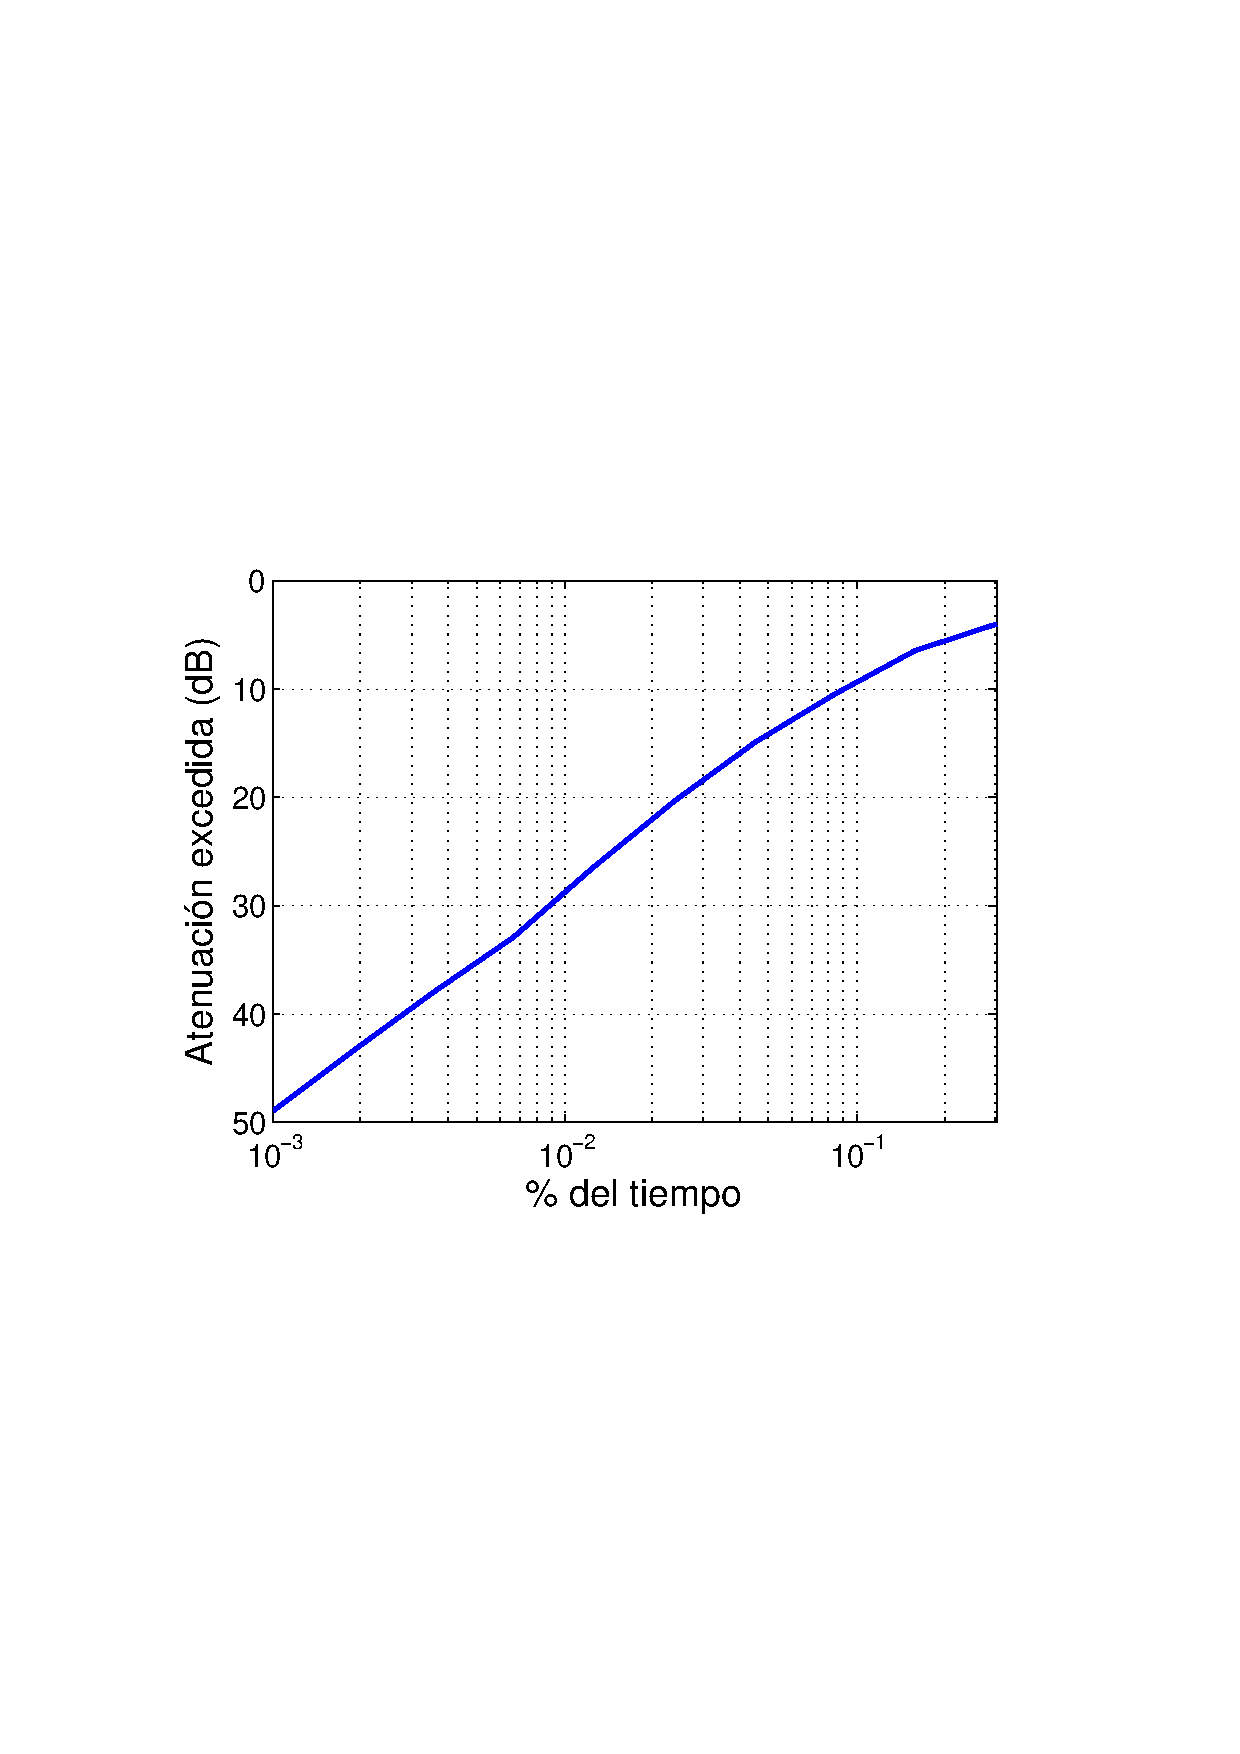
\includegraphics[width=8 cm]{CapituloProblemasLibroETSI/figuras/rain13GHz.pdf}
\caption{Atenuación por lluvia excedida en el $p$ \% del tiempo para 13 GHz y 15 km de distancia}\LABFIG{resfFHop13}%\vspace{-.5 cm}
\end{figure} 

 \begin{solnum}
 \item 
En principio la frecuencia de trabajo no es muy alta, lo que hace pensar que el enlace no estará limitado por lluvia. Los tiempos medios entre fallos son grandes, lo que parece indicar que la indisponibilidad, o interruciones largas, no va a ser un problema. Mientras que sí lo será la pérdida de fidelidad, o interrupciones breves. En todo caso, como el régimen binario es bajo, $\leq 34$ Mbps, el desvanecimiento selectivo no es importante. 

El margen bruto es el que domina en ambos criterios de calidad. De forma que podemos calcular el margen necesario para que se cumplan los objetivos de interrupciones largas (indisponibilidad) y cortas (fidelidad) y quedarnos con el más restrictivo, el mayor.

Calculamos primero el margen necesario para que se cumpla la indisponibilidad. La indisponibilidad de equipos sería la resultante de la suma de la indiponibilidad en cada extremo. En cada extremo tenemos dos equipos funcionando, la IU y la OU, el $MTBF$ equivalente es
\begin{align}
MTBF_e&=(MTBF_{IU}^{-1}+MTFB_{OU}^{-1})^{-1}\nonumber\\
    &=((110\cdot24\cdot 365)^{-1}+(35\cdot24\cdot365)^{-1})^{-1}=2.3259\cdot 10^5.
\end{align}
 Y calculamos
\begin{align}
q&=MTTR/(MTTR+MTBF_e)=20/(20+2.3259\cdot 10^5)=8.5980\cdot 10^{-5}.
\end{align}
 para finalmente estimar la indisponibilidad
\begin{align}
U_{e}&=2 \cdot 100\cdot \binom{M+N}{N+1} (mq)^{N+1}\nonumber\\&=2\cdot 100 \cdot\binom{1+1}{1+1} (1\cdot 8.5980\cdot 10^{-5})^{1+1}
=1.478510^{-6}\%,
\end{align}
%Si no se tuviese HSB, tendríamos 
donde $m=1$ porque tenemos un vano y  $M=N=1$ porque el HSB (Hot Stand By) es $M+N=1+1$. Dado que el máximo valor permitido es $0.036\%$ y que el valor anterior de indisponibilidad por equipos es muy muy pequeño, el máximo valor permitido para indisponibilidad por propagación es, aproximadamente este mismo valor (...)\end{solnum}



%%%%%%%%%%%%
%%%%%%%%%%%%
%%%%%%%%%%%%

\problema{Radioenlace del servicio fijo a 13 GHz}

Una compañía de telefonía móvil desea instalar un radioenlace digital del servicio fijo a $13$ GHz, para unir dos estaciones base a través de un vano de $15$ km de longitud. El enlace tiene un obstáculo agudo de incidencia rasante, esto es, con despejamiento $h=0$ y que introduce unas pérdidas de 6 dB a la par que evita cualquier reflexión en el suelo. 

Se propone utilizar para ello equipos de la serie Flexi-Hopper de Nokia, cuyos datos se incluyen en la \TAB{resfFHop13} para una transmisión dúplex\footnote{ el $2\times$ indica que se utilizan las dos polarizaciones para transmitir.} de $2 \times 2$E1, resultando $4.2$ Mbps en cada sentido modulados en un radiocanal. Tanto el transmisor como el receptor constan de una unidad interior (IU), al pié de la torre, y una unidad exterior (OU) con la etapa de RF junto a la antena, en el extremo superior de las torres, de 15 m. Se sabe, además, que hay una probabilidad $\eta = 25.73$ \% de que exista actividad multitrayecto en el vano para esa zona climática. Además, para esa zona climática se conoce la atenuación, $A_p$, excedida en el $p$\% del tiempo, ver \FIG{resfFHop13}. 

El operador ha fijado como criterios de calidad el \% del tiempo en el que el sistema sufre interrupciones largas y cortas, y como objetivos que las primeras ($>10$s, $BER>10^{-3}$) no superen el $0.036\%$ y las cortas ($\leq10$s, $BER>10^{-3}$) no superen el 0.006\% anual. El departamento de radio tiene que calcular la mínima potencia transmitida para la que el enlace es viable, evitando así interferencias a otros sistemas. 
 
Se pide 
\begin{enumerate}%[labelindent=\parindent,leftmargin=\parindent, label=\normalfont\bfseries  \alph*)] 
\item Calcular el valor de esta potencia. Indique si es necesario mantener en el diseño el HSB (Hot Stand By).
\end{enumerate}   

\begin{table}[h]
%\small
\caption{Datos de las estaciones, con equipos Flexi-Hopper de Nokia}
\begin{center}
\begin{tabular}{p{8.5cm}p{2.5cm}}
 \hline
Potencia transmitida	(entregada a antena) regulable & -5 a 20 dBm	\\
Ganancia antenas & $40.5$ dBi\\	
Modulación & $\pi/4$-DQPSK\\
%Pérdidas en conectores 1 dB	\\
Potencia recibida necesaria para  $BER = 10^{-3}$ y 2E1 ($4.2$Mbps) & $P_{dr}=-89$ dBm\\
Figura de ruido del sistema & 6 dB\\
HSB 1+1, tanto en OU e IU &\\
Tiempo medio entre fallos para OU & $MTBF$=35 años \\
Tiempo medio entre fallos para IU $MTBF$=110 años \\
Tiempo medio en reparar para OU como IU & $MTTR$=20 horas\\
%Altura de antenas sobre el suelo, 15 m\\
Signatura normalizada del receptor	& $k = log_2 M$ \\
 $M$ el número de puntos de la constelación de la modulación & \\
 \hline
\end{tabular}
\end{center}
\LABTAB{resfFHop13}
\end{table}%
\begin{figure}[h]
\centering 
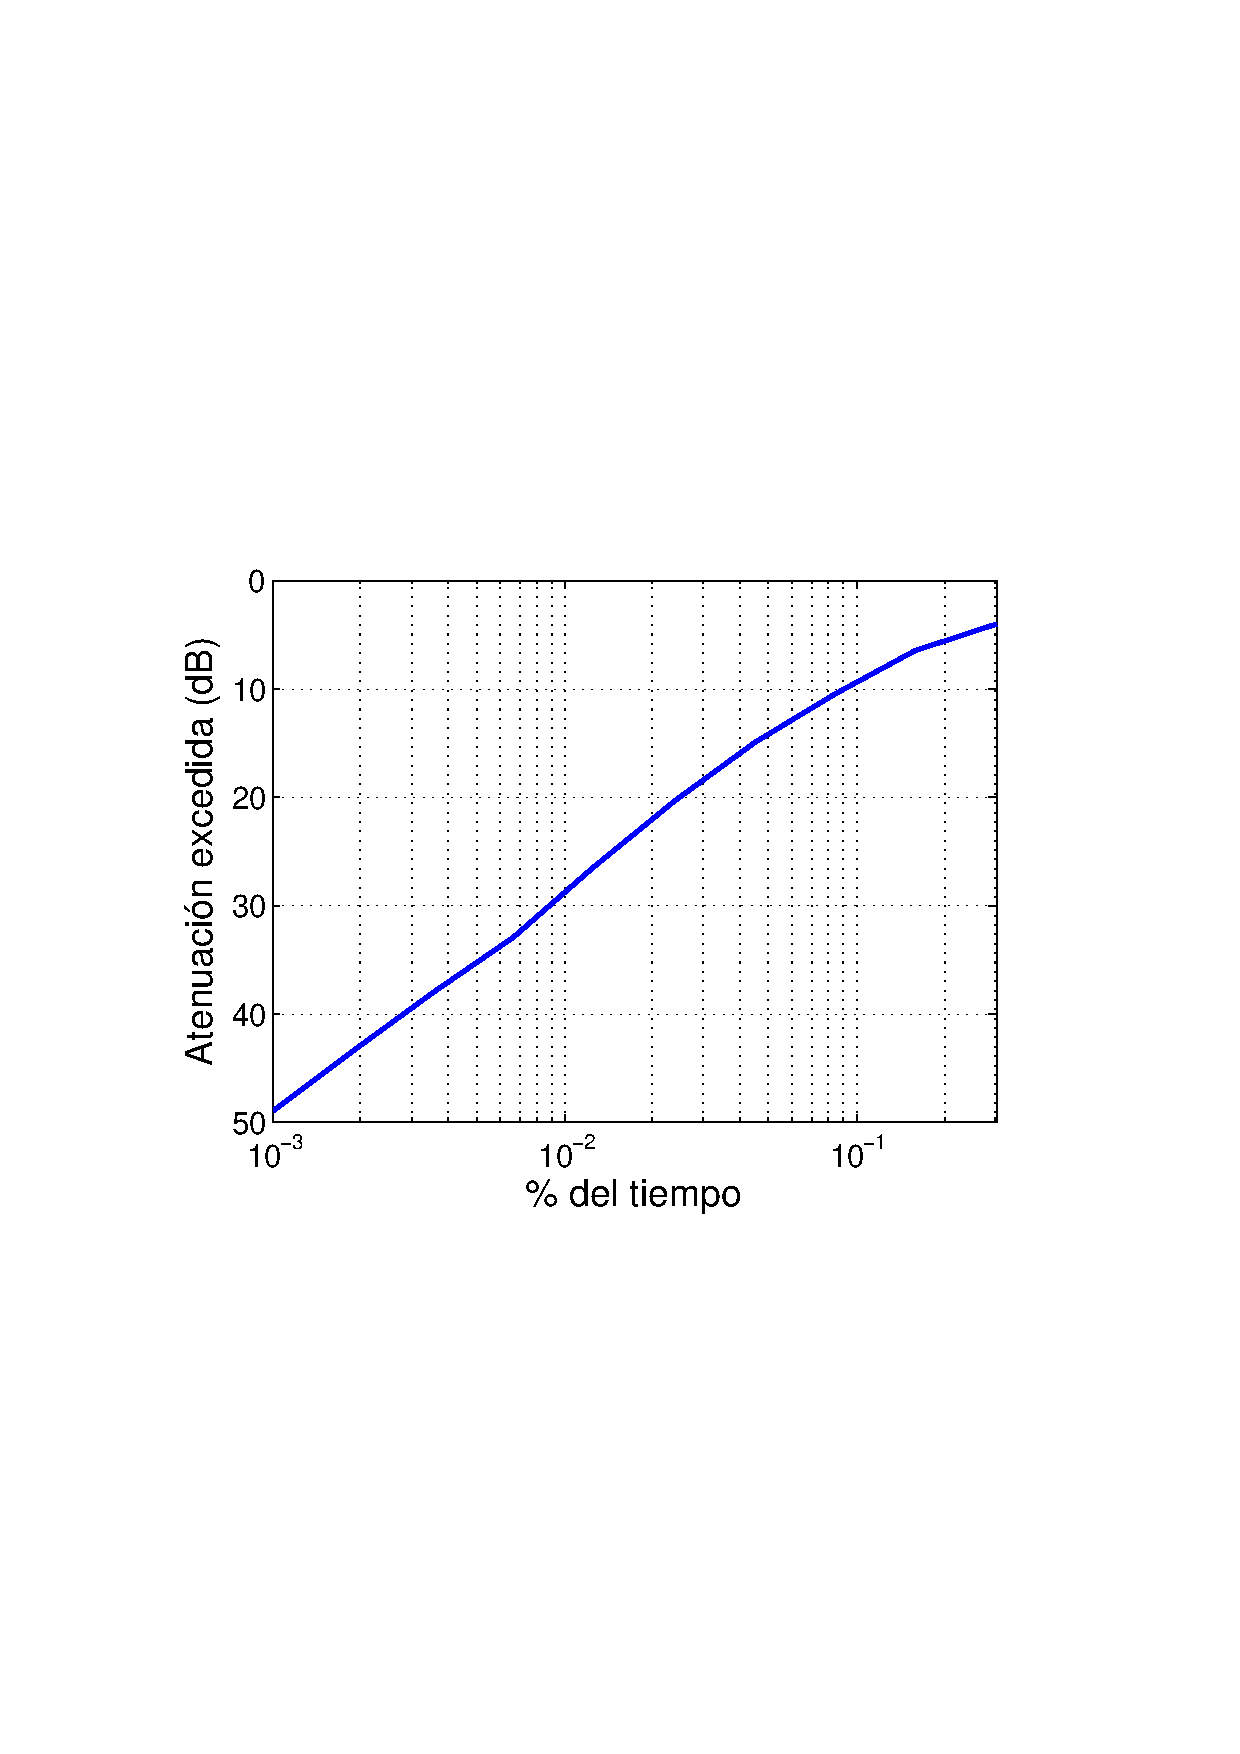
\includegraphics[width=8 cm]{CapituloProblemasLibroETSI/figuras/rain13GHz.pdf}
\caption{Atenuación por lluvia excedida en el $p$ \% del tiempo para 13 GHz y 15 km de distancia}\LABFIG{resfFHop13}%\vspace{-.5 cm}
\end{figure} 

%%%%%%%%%%%
%%%%%%%%%%%
%%%%%%%%%%%

\section{...Ruido y sensibilidad}\LABSEC{Ruido}
Vamos a estudiar el ruido y la sensibilidad en ...

\subsection{...Temperatura y figura de ruido} \LABSSEC{Ruido}
En este texto, ver comienzo del mismo, se denota por $f_r$ y $T_r$ la figura y la temperatura equivalente de ruido, respectivamente, del receptor, formado éste por los elementos que van desde el conector de antena a la entrada al demodulador. Por otro lado, $f_a$ y $T_a$ se utilizan para denotar la figura y la temperatura equivalente de ruido de la antena. Y $f_s$ y $T_s$ denotan la figura de ruido y la temperatura equivalente del sistema completo, antena más receptor.  Aquí las figuras de ruido están en unidades naturales, y las denotamos por ello en minúsculas. La misma notación para las figuras de ruido en mayúsculas se utilizará para denotar dB. (...)%Por otra parte, se asume adaptación de impedancias en el sistema. 

\subsection{...Temperatura y figura de ruido} \LABSSEC{Ruido}
... En este texto, ver comienzo del mismo, se denota por $f_r$ y $T_r$ la figura y la temperatura equivalente de ruido, respectivamente, del receptor, formado éste por los elementos que van desde el conector de antena a la entrada al demodulador. Por otro lado, $f_a$ y $T_a$ se utilizan para denotar la figura y la temperatura equivalente de ruido de la antena. Y $f_s$ y $T_s$ denotan la figura de ruido y la temperatura equivalente del sistema completo, antena más receptor.  Aquí las figuras de ruido están en unidades naturales, y las denotamos por ello en minúsculas. La misma notación para las figuras de ruido en mayúsculas se utilizará para denotar dB. (...)%Por otra parte, se asume adaptación de impedancias en el sistema. 

\subsection{...Temperatura y figura de ruido} \LABSSEC{Ruido}
... En este texto, ver comienzo del mismo, se denota por $f_r$ y $T_r$ la figura y la temperatura equivalente de ruido, respectivamente, del receptor, formado éste por los elementos que van desde el conector de antena a la entrada al demodulador. Por otro lado, $f_a$ y $T_a$ se utilizan para denotar la figura y la temperatura equivalente de ruido de la antena. Y $f_s$ y $T_s$ denotan la figura de ruido y la temperatura equivalente del sistema completo, antena más receptor.  Aquí las figuras de ruido están en unidades naturales, y las denotamos por ello en minúsculas. La misma notación para las figuras de ruido en mayúsculas se utilizará para denotar dB. (...)%Por otra parte, se asume adaptación de impedancias en el sistema. 

%Para incluir otro problema, utilice \problema
\endinput
 
 
% !TEX root =../LibroTipoETSI.tex

%:Descripción del fichero de estilo de la ETSI

\chapter{Estilo tipográfico LibroETSI}\label{estilo}

\lettrine[lraise=-0.1, lines=2, loversize=0.25]{E}{n} este Capítulo se analiza el fichero de estilo \ttcolor{libroETSI.sty} en el que se han definido los diferentes elementos que constituyen el estilo tipográfico propuesto en la Escuela Técnica Superior de Ingeniería de la Universidad de Sevilla para la redacción y publicación de libros y otros tipos de documentos. 

El objetivo de este análisis es explicar detalladamente la relación entre los paquetes que se han utilizado y su reflejo en la confección del documento, para permitir, si se desea, modificar, corregir o mejorar cualquiera de los mismos por los usuarios.

Por supuesto, como ocurre en cualquier diseño, existen propuestas alternativas a las que aquí se recogen y creemos que con la exposición realizada se facilitará una mayor extensión de la utilización de \LaTeX\ por parte de todos los miembros de nuestra Escuela. 

Es importante señalar que muchas de las instrucciones del estilo \emph{tienen que estar en el orden que se proponen}. Al ser \LaTeX\ un lenguaje en el que numerosos bloques de código (paquetes) se cargan consecutivamente, es importante el orden en el que se realiza esta carga, para evitar posibles incompatibilidades.

\section{Bloque 0}

Está formado por un conjunto de sentencias genéricas en cualquier hoja de estilo de \LaTeX\ y en él se establece el formato que va a utilizarse (LaTex2e) además de definir las posibles opciones que se han incorporado al estilo y procesarlas. Debemos observar que estas opciones pueden venir definidas o bien en la declaración del documento, como se propone en el fichero \ttcolor{libroTipoETSI.tex} o bien en la propia llamada del paquete. Así, se podrían haber escrito las primeras instrucciones del fichero \ttcolor{libroTipoETSI.tex} en la forma:

\begin{lstlisting}[rulecolor=\color{white}]
\documentclass[paper=a4,10pt, twoside]{scrbook}
\usepackage[Myfinal=true, Minion=false]{libroETSI}
\end{lstlisting}

Para poder utilizar estas opciones y alguna otra que veremos interesante introducir, como el idioma, debemos saber que, por defecto, son falsas por lo que, en realidad, no hubiera sido necesaria colocar la opción \ttcolor{Minion=false}. Sin embargo, a veces se prefiere su declaración para hacer más explícita que se está utilizando. Observar la forma que se definen las opciones mediante las instrucciones

\begin{lstlisting}[rulecolor=\color{white}]
\DeclareBoolOption{Myfinal}
\DeclareBoolOption{Minion}
\DeclareBoolOption{English}
\end{lstlisting}

\section{Bloque 1: Aspectos generales}

El primer paquete que se carga se denomina \ttcolor{etoolbox}. \index{etoolbox}Este paquete general permite importantes correcciones en el resto de la hoja de estilo, modificando de manera sustancial el comportamiento de algunos de los elementos utilizados. Así, por ejemplo, hemos utilizado un comando definido en este paquete, \ttcolor{appto} \index{appto}en la sentencia

\begin{lstlisting}[rulecolor=\color{white}]
\appto{\appendices}{\def\Hy@chapapp{Appendix}}
\end{lstlisting}
que ha resuelto un grave problema que aparece al generar el índice de un documento que tenga apéndices que esté escrito en español o cualquier otro idioma que tenga caracteres no comprendidos entre los primeros 128 del código ASCII.

A continuación se cargan un conjunto de paquetes que resuelven incompatibilidades con el tipo de documento que estamos utilizando, resuelven problemas internos o nos permiten realizar comparaciones booleanas. 

Seguidamente se carga el paquete \ttcolor{microtype}\index{microtype}, si el parámetro \ttcolor{Myfinal} es \ttcolor{true}. Este paquete es responsable de finísimos microajustes en los textos generados por \LaTeX\, permitiendo la expansión o comprensión de caracteres y espacios en blanco de un documento para mejorar su apariencia. Con diferencia a lo que se realiza en Word, \TeX\ gestiona estas correcciones a nivel de parágrafo, lo que confiere un aspecto altamente profesional a los documentos generados. Debido a la complejidad de los algoritmos que se utilizan, al cargar \ttcolor{microtype} se enlentece considerablemente la compilación del documento, por lo que resulta conveniente definir \ttcolor{Myfinal} como \ttcolor{true} únicamente en las etapas últimas de redacción. ¡Pero no sólo en la última!, puesto que el ajuste que introduce hace que a veces cambie la situación de las líneas huérfanas y viudas, de considerable importancia desde un punto de vista tipográfico. 

Siguiendo los consejos de los editores de IEEE, se han modificado un conjunto de valores por defecto lo que hace el documento menos restrictivo en lo referente a la colocación de los elementos flotantes dentro de una página. Además, se ha optado por permitir que un conjunto de fórmulas que constituyan un bloque (definidas dentro del entorno  \comandos{begin}{align}... \comandos{end}{align}, por ejemplo) puedan escribirse en diferentes páginas. Si se desea cambiar este comportamiento, simplemente debemos modificar el valor de \ttcolorc{interdisplaylinepenalty} a un valor más elevado, por ejemplo $10000$.

Aunque el tipo de documento utilizado, \ttcolor{scrbook}\index{scrbook}, incorpora por defecto un conjunto de instrucciones que permiten una gestión muy eficiente del tamaño de los diferentes elementos que constituyen una página (cabecera, ancho del texto, altura, pie de página, offset de encuadernación, etc, ) se ha optado por utilizar el paquete \ttcolor{geometry}\index{geometry} para ese fin. En el fichero de estilo simplemente se carga el paquete y los parámetros concretos se definen posteriormente en el fichero principal que estemos utilizando. Por ejemplo, este documento se ha generado con los siguientes:

\begin{lstlisting}[rulecolor=\color{white}]
paperheight=240mm,% Altura de la página
paperwidth=170mm,%   Anchura
top=25mm,%
headsep=7.5mm,%
footskip=10mm,%
textheight=190mm,%     Altura del texto
textwidth=124mm,%      Ancho del texto
bindingoffset=15mm,%   Offset de encuadernación
twoside
\end{lstlisting}

Finalizamos este bloque definiendo un alias para el tamaño básico de la fuente que hemos declarado en la sentencia inicial para poder realizar un escalado de los diferentes tamaños que se van a usar en el documento. Observad que se crean dos dimensiones, para la fuente y para el interlineado. \ttcolorc{lnormal} y \ttcolorc{lbnormal}, respectivamente.

\section{Bloque 2: Idioma, Codificación y Fuentes}
\subsection{Idioma}
La posibilidad de utilizar nuestra plantilla para escribir textos en inglés (es el único idioma aparte del español que se ha considerado) nos obliga a establecer una posible opción para cargar el paquete \ttcolor{babel}\index{babel} de una u otra manera. Este paquete es el responsable de establecer las reglas de partición silábica, entre otras cosas, por lo que resulta imprescindible su incorporación a una hoja de estilo. Cabe decir que en estos momentos el responsable de su mantenimiento es el español Javier Bezos, lo que nos garantiza una excelente adaptación del paquete a nuestro idioma.

Además de la partición silábica, un determinado conjunto de macros quedan automáticamente traducidos como por ejemplo, la definición de límite, máximos y mínimos que se utilizan en la escritura matemática. Observemos cómo aparecen unos y otros en función del idioma que utilicemos:
\begin{LTXexample}[pos=r, hsep=15pt,width=0.45\textwidth]
\begin{align*}
\lim_{n\to\infty}a_{n}&=10\\
\max\left[{a,b}\right]&=a
\end{align*}
\figurename, \tablename

\selectlanguage{english}
\begin{align*}
\lim_{n\to\infty}a_{n}&=10\\
\max\left[{a,b}\right]&=a
\end{align*}
\figurename, \tablename
\selectlanguage{spanish} 
\end{LTXexample}

El grupo de macros que gestionan los nombres que cambian en uno y otro caso, se encuentra a continuación en el fichero de estilo. 
\subsection{Codificación}
Para gestionar la forma en la que se controla la codificación en la que está escrita los ficheros fuentes de \LaTeX\ se utiliza el paquete \ttcolor{inputenc}\index{inputenc} junto con el paquete \ttcolor{fontenc}\index{fontenc}. Estos dos paquetes sólo son necesarios si no utilizamos \LuaLaTeX\ ya que en caso de utilizarse este motor, la gestión se realiza por un mecanismo completamente diferente, interno al propio motor y del que podemos despreocuparnos. 

\subsection{Fuentes del texto y comandos asociados}
La selección de la fuente a utilizar depende fundamentalmente de qué motor estemos utilizando para generar nuestro texto. Si optamos por \LaTeX\ (en realidad, pdf\LaTeX\ ), la selección del texto normal se realiza en el fichero principal mediante el comando \comandos{usepackage}{tgtermes}, que selecciona para el texto un clon de la fuente Times. En general, las fuentes que se pueden utilizar con \LaTeX\ no son demasiadas y una excelente recopilación de las disponibles se encuentra en la dirección \url{http://www.tug.dk/FontCatalogue/}. 

Sin embargo, si nuestro motor es \LuaLaTeX, podemos utilizar como fuente de texto cualquier fuente .otf ó .ttf presente en nuestro ordenador. Cómo se cargan dichas fuentes y cómo se utilizan se encuentra recogido en la documentación del paquete \ttcolor{fontspec}\index{fontspec} y en nuestro estilo se muestra en las líneas de código siguientes:
\begin{lstlisting}[rulecolor=\color{white}]
\setmainfont[Renderer=Basic, Ligatures=TeX,% 
	Scale=1.0,%
	]{Times New Roman}
\end{lstlisting}

La fuente que hemos seleccionado de esta manera es la que utilizaremos en el texto normal. Es decir, en todo el texto que no sea cabeceras de página, enunciados de secciones, captions de figuras, etc. Para todos estos casos, como una elección de diseño, hemos utilizado una fuente perteneciente al tipo denominado \emph{sin serif}. En el caso de \LaTeX\ hemos optado por una fuente {\ifluatex{\fontspec[Scale=0.95]{Helvetica}Helvética Narrow}\else{Helvética Narrow}\fi}, mientras que en el caso de \LuaLaTeX\ hemos utilizado una fuente {\ifluatex{\fontspec{Arial Narrow}Arial Narrow}\else{Arial Narrow}\fi}. Los comandos iniciales de esta decisión se muestran en las siguientes líneas de código.
\begin{lstlisting}[rulecolor=\color{white}]
\ifluatex
	\setsansfont[Ligatures=TeX,		% Se puede obtener un texto sin serif con \ssfamily				
	Scale=0.95,
	]{Arial Narrow}
\else
	\renewcommand{\sfdefault}{phv} 
\fi
\end{lstlisting}

Podemos observar la sintaxis completamente diferente que se utiliza en un caso y otro.  En realidad, para facilitar la utilización de diversas variantes de ambas fuentes, en cualquiera de los dos motores de composición elegidos, hemos definido un conjunto de comandos que están recogidos en las siguientes líneas.

\begin{lstlisting}[rulecolor=\color{white}]
\ifluatex

	\newfontfamily\helveticam{Arial}						% Helvética
	\newfontfamily\helveticab{Arial Bold}					% Helvética Bold
	\newfontfamily\helveticai{Arial Italic}					% Helvética itálica
	\newfontfamily\helveticax{Arial Bold Italic}				% Helvética Bold Itálica

	\newfontfamily\titular{ArialNarrow-Bold}				% Para los titulares
	\newfontfamily\titulart{ArialNarrow-Bold}				% Para los titulos
	\newfontfamily\titulari{ArialNarrow-BoldItalic}			% Para los titulares oblicua

	\newfontfamily\titulartoc{ArialNarrow}					% Para el TOC
	\newfontfamily\titulartocb{ArialNarrow-Bold}			% Para el TOC bold
	\newfontfamily\titulartoci{ArialNarrow-BoldItalic}		% Para el TOC oblicua

\else

	\newcommand{\helveticam}{\usefont{T1}{phv}{m}{n}\selectfont }
	\newcommand{\helveticab}{\usefont{T1}{phv}{b}{n}\selectfont }
	\newcommand{\helveticai}{\usefont{T1}{phv}{m}{it}\selectfont }
	\newcommand{\helveticax}{\usefont{T1}{phv}{b}{it}\selectfont }

	\newcommand{\titular}{\usefont{T1}{phv}{bc}{n}\selectfont }
	\newcommand{\titulari}{\usefont{T1}{phv}{bc}{it}\selectfont }
	\newcommand{\titulart}{\usefont{T1}{phv}{bc}{n}\selectfont }
	
	\newcommand{\titulartoc}{\usefont{T1}{phv}{mc}{n}\selectfont }
	\newcommand{\titulartocb}{\usefont{T1}{phv}{bc}{n}\selectfont }
	\newcommand{\titulartoci}{\usefont{T1}{phv}{mc}{it}\selectfont }
	
\fi
\end{lstlisting}

De esta manera para el usuario del paquete es transparente el uso de \LaTeX\ o \LuaLaTeX . La sintaxis en este último caso se debe a la utilización del paquete \ttcolorc{usepackage[no-math]\{fontspec\}} que hemos cargado con anterioridad y en el caso de \LaTeX\ al uso de instrucciones básicas del esquema de selección de fuentes.

En cualquier caso, hasta este momento sólo hemos definido los comandos que nos permitirán hacer uso de las tipografías seleccionadas. Su aplicación concreta, con el tamaño que hemos elegido debe realizarse a continuación. En primer lugar, para facilitar un escalado adecuado de las distintas fuentes, hemos definido un conjunto de dimensiones relativas como, por ejemplo,
\begin{lstlisting}[frame=none]
\newdimen\lcatorce
\newdimen\lbcatorce
\end{lstlisting}
y posteriormente le hemos asignado valores, 
\begin{lstlisting}[frame=none]
\lcatorce=\dimexpr1.4\dimexpr\lnormal
\lbcatorce=\dimexpr1.4\dimexpr\lbnormal
\end{lstlisting}

Estos valores se corresponden  en este caso a fracciones (1,4 ó 140\%) del tamaño de la fuente normal que, recordemos, habíamos definido con anterioridad.

Por último, un conjunto de comandos facilita la utilización de las fuentes en sus diversas variaciones a lo largo de todo el texto. Así, por ejemplo, se ha definido en la siguiente línea de código un comando para definir la fuente y el tamaño que vamos a usar en los títulos de las secciones:
\begin{lstlisting}[frame=none]
\newcommand{\aheadsecc}{\fontsize{\ltrece}{\lbtrece} \titular}
\end{lstlisting}

Por supuesto, una vez que hemos definido este comando, podemos utilizarlo siempre que deseemos. Así, la utilización y el resultado del comando \ttcolorc{aheadsecc} se muestra a continuación:
\begin{LTXexample}[pos=r, hsep=15pt,width=0.45\textwidth]
\aheadsecc{Como si fuera una sección}
\end{LTXexample}

\subsection{Fuentes matemáticas y símbolos}
En una Escuela de Ingeniería la gestión de las fuentes matemáticas en nuestros documentos juega un papel fundamental. Po ello, si utilizamos \LuaLaTeX\ es necesario cargar los paquetes \ttcolor{lualatex-math}\index{lualatex-math} y \ttcolor{luatextra}\index{luatextra}. Observar además que aparte de estos dos paquetes, orientados básicamente a la utilización de aspectos concretos relacionados con símbolos matemáticos, hemos incluido el comando \ttcolorc{usepackage[no-math]\{fontspec\}}. Aunque \ttcolor{fontspec} se utilizará en la gestión del tipo de fuentes y comandos relacionados con las mismas, es necesario incluirlo aquí por el típico problema que hemos mencionado anteriormente del orden en el que se encargan los paquetes.

En general, para mejorar el escalado de determinados símbolos, utilizaremos el paquete \ttcolor{exscale}\index{exscale}. Advertimos nuevamente que \emph{se tiene que cargar exactamente antes que el paquete \ttcolor{amsmath}\index{amsmath}}, que se carga a continuación, junto con una adición recomendable, el paquete \ttcolor{mathtools}\index{mathtools}.

Existen numerosos paquetes que definen los símbolos matemáticos más habituales. Uno de los más completos es el paquete \ttcolor{MnSymbol}\index{MnSymbol}, especialmente indicado cuando la fuente del texto es la Minion, licenciada por Adobe. Sin embargo, la utilización tanto de la fuente de símbolos como la fuente de texto dentro de \LaTeX\ es un asunto no trivial. Requiere la disponibilidad de la fuente Minion, y la creación del  paquete \ttcolor{MinionPro}\index{MinionPro}. El lector interesado puede encontrar el procedimiento para crear dicho paquete en \url{https://github.com/sebschub/FontPro/}.

Si se han seguido las instrucciones que se encuentran en la dirección anterior y se desea utilizan la fuente, se indicará mediante uno de las opciones del programa, escribiendo \ttcolor{Minion=true}. Con ello, se cargarían los correspondientes paquetes mediante las primeras líneas del siguiente código:
\begin{lstlisting}[rulecolor=\color{white}]
\makeatletter
\ifdtsc@Minion
	\usepackage{MnSymbol}
	\usepackage[mathlf, minionint, mnsy]{MinionPro}
	\newcommand{\bm}{\ensuremath{\boldsymbol}}
\else
	\usepackage{amssymb}
	\usepackage{mathptmx}
	\usepackage{amsfonts}
	\usepackage{bm}
\fi
\makeatother
\end{lstlisting}

En el caso que no se tenga instalado el paquete, o no se desee utilizar, basta ignorar la opción y se ejecutarán las restantes líneas del código anterior. 

\section{Bloque 3: Tabla de contenidos}
Uno de los aspectos sobresalientes de \LaTeX\ es la facilidad para generar la \emph{Tabla de contenidos} (TOC) de un documento. No sólo para generarla sino también para controlar cómo se presenta y cómo se gestiona el contenido de la misma. En esta sección explicaremos los comandos que hemos utilizado con este fin, teniendo en cuenta que hemos actuado directamente renombrado y creando nuevos elementos, sin utilizar paquetes específicos para esta tarea. Si alguno desea hacer uso de los mismos, unos de los más ampliamente utilizados es el paquete \ttcolorc{tocloft}\index{tocloft}.

Para controlar dónde queremos que aparezca la tabla de contenido, debemos utilizar el comando \ttcolorc{tableofcontens}\index{tableofcontens}. Si analizamos el fichero principal de este documento, veremos que precediendo a este comando aparecen las líneas
\begin{lstlisting}[frame=none]
\cleardoublepage
\phantomsection
\addcontentsline{toc}{listasf}{Índice}
\pagestyle{especial}
\end{lstlisting}
Con ellas indicamos, en primer lugar, que la tabla de contenidos siempre va a aparecer en una página impar, que haremos uso de un estilo de página\footnote{Más adelante veremos cómo se definen estos estilos.} que denominamos \ttcolor{especial} y que queremos que la propia tabla de contenido (o índice del documento) aparezca referenciada en en el índice, aunque pueda parecer complejo entender lo que esto significa.\LaTeX\ permite controlar el nombre que le hemos asignado a la tabla de contenido mediante la sentencia \comando{def}\comando{contentsname}\ttcolor{\{Índice\}}, tal como se define en otro lugar del estilo, puesto que este nombre dependerá del idioma que utilicemos.
 
A la hora de construir esta tabla de contenidos, nuestra primera decisión fue establecer que iban a aparecer hasta los apartados que hemos denominados \ttcolor{subsubsecciones}, lo que se logra mediante el \ttcolor{\{3\}} del comando \comandos{setcounter}{tocdepth}\index{tocdepth} en \ttcolor{libroETSI.sty}.  Cambiar este número haría aparecer menos apartados o más, dependiendo de la elección.

Para establecer la manera en la que cada nivel de segmentación aparece en el TOC hacemos uso de una secuencia de comandos similares a las mostradas a continuación para el caso del capítulo:
\begin{lstlisting}[frame=none, numbers=left, xleftmargin=2em]
\makeatletter
	\renewcommand*\l@chapter[2]
	{
    \addpenalty{-\@highpenalty}%
    \vskip 0.5em \@plus\p@
	 \@dottedtocline{0}{0em}{1em}{\tocchap #1}{\tocchap #2}
	}
\makeatother
\end{lstlisting}
El elemento clave está recogido en la línea \ttcolor{6}. El significado de cada uno de los parámetros es el siguiente: el \ttcolor{0} señala que estamos formateando el nivel de capítulo. El siguiente parámetro, \ttcolor{0em} establece la indetación de la línea, \ttcolor{1em} define la anchura que reservamos para el número que mostramos, si es que la parte tiene números y los otros dos establecen las características tipográficas que vamos a utilizar para el título (incluyendo el número si lo hubiera) y el número de la página en el que se encuentra la correspondiente parte. Este ajuste se ha realizado sin tener en cuenta ninguno de los paquetes, únicamente utilizando sentencias del propio núcleo de \LaTeX\. De forma similar hemos procedido para el resto de los elementos de segmentación del texto.

Aunque algo redundante, nuestra siguiente decisión afecta a la manera en la que hemos querido que aparezcan en el índice los índices del texto (valga la redundancia), tales como el \emph{Índice de Figuras}, \emph{Índice Alfabético}, etc y otros elementos como el \emph{Resumen, Prefacio}, etc o la \emph{Bibliografía}. No es trivial pero, básicamente, hemos definido dos listas, una para los elementos que aparecen antes del Índice y otra para los  que aparecen después, al final del texto, que se corresponden aproximadamente a lo que hemos denominado \ttcolorc{frontmatter}\index{frontmatter} y \ttcolorc{backmatter}\index{backmatter}, respectivamente. Si nos fijamos por ejemplo en la lista que hemos denominado \ttcolorc{listasf}, cómo se representan los elementos que están incluidos en la misma se realiza con las instrucciones
\begin{lstlisting}[frame=none]
\makeatletter
	\newcommand*\l@listasf[2]
	{
    \addpenalty{-\@highpenalty}%
    \vskip 0.05em \@plus\p@
	 \@dottedtocline{0}{0em}{2.5em}{\fontsize{\lnueve}{\lbnueve}\selectfont \helveticai #1}{\fontsize{\lnueve}{\lbnueve}\titulartoc #2}
	}
\makeatother
\end{lstlisting}
en las que vemos, por ejemplo, que el tamaño del texto es el tamaño relativo \ttcolorc{lbnueve}, junto con una fuente \ttcolorc{helveticai} represente esta fuente lo que represente (en un apartado anterior ha quedado definido).

Una cuestión distinta es las instrucciones que debemos ejecutar para incluir un determinado elemento en la lista correspondiente. Por ejemplo, para incluir el \emph{Prefacio} en la  \ttcolorc{listasf}, observemos que hemos escrito el siguiente comando: 
\begin{lstlisting}[frame=none]
\addcontentsline{toc}{listasf}{Prefacio}
\end{lstlisting}

Para finalizar este apartado, también hemos propuesto que no aparezcan los habituales puntos que existen entre el texto y el número de página correspondiente de muchos índices, ajustando a \ttcolor{10000} el parámetro \ttcolor{\textbackslash@dotsep}. Unas referencias interesantes para manejar todos estos elementos las encontramos en las siguientes direcciones \url{http://tex.stackexchange.com/questions/110253/what-the-first-argument-for-lsubsection-actually-is} y \url{http://tex.stackexchange.com/questions/33841/how-to-modify-the-indentation-before-sectioning-titles-in-the-table-of-contents}.

\section{Bloque 4: Estilos de Páginas y Títulos}
Este apartado ha sido uno de los más complejos en cuanto a diseño se refiere, atendiendo a la gran cantidad de elementos que componen un texto y sus interrelaciones. 

En general, se recomienda que los tipos de páginas diferentes que se utilicen en un documento sea un número muy limitado. Por ello, \LaTeX\ no establece un mecanismo elemental para definir distintos tipos de páginas (en realidad, únicamente un tipo \ttcolor{plain} y un tipo \ttcolor{empty}) y debemos acudir a paquetes específicos que nos permitan una mayor libertad de diseño. Lo mismo podríamos decir a la hora de definir el formato de los distintos elementos, lo que hemos denominado genéricamente \emph{Títulos}, haciendo con ello referencia a los \emph{Títulos} de los capítulos, secciones, subsecciones, etc. 

Hemos de tener en cuenta que el aspecto de un libro está básicamente determinado por el formato que se ha elegido para los diferentes títulos de las partes que lo constituyen, el formato de las páginas y qué queremos que aparezca en las cabeceras y pies de páginas del mismo. Todo esto se ha conseguido utilizando un paquete desarrollado por el español Bezos denominado \ttcolor{titlesec}\index{titlesec}, que se carga en nuestro fichero mediante la instrucción \comandos{usepackage[noindentafter, pagestyles,...]}{titlesec}. En el listado siguiente se recogen algunos de los elementos de los formatos elegidos para que mediante su análisis podamos realizar nuestro propio diseño.
\begin{lstlisting}[frame=none, numbers=left, xleftmargin=2.5em]
\newpagestyle{esitscCD}
	{
	\esirulehead
	\sethead[\numpagpar \rhfont\chaptername\ \thechapter. \;\chaptertitle][][]%
			{}{}{\rhfont\thesection\ \;\sectiontitle \numpagodd}
	}

\newpagestyle{primera}
	{
	\esirulehead \footrule
  	\sethead[][][]{\includegraphics[width=2 cm]{logoUS.pdf}}%
  				{\raisebox{0.8cm}{\begin{minipage}{0.515\textwidth}
				\centering
				{\aheadsubsecc \fromtitulacion}\\
				\vspace*{.5ex}
				{\normalfont \fromasignatura}\\
				\vspace*{1ex}
				\normalfont \fromconvocatoria \quad \fromfecha
				\end{minipage}}
				}%
				{\includegraphics[width=4 cm]{logoTSC.pdf}
				}
	\setfoot{}{\rhpagefont Pág. \thepage\, de\, \zpageref{LastPage}}{}
  	}

\newpagestyle{examen}
	{
	\esirulehead
	\sethead[\rhpagefont Pág. \thepage\, de\, \zpageref{LastPage}][\aheadsubsecc\fromasignatura][[\rhpagefont\fromfecha]%
	{[\rhpagefont\fromfecha}{\aheadsubsecc\fromasignatura}{\rhpagefont Pág. \thepage\, de\, \zpageref{LastPage}}
	}

\newpagestyle{problema}
	{
	\esirulehead
    	\sethead[\numpagpar][][\rhfont\chaptername \; \thechapter. \chaptertitle]% even
        		{\rhfont\theproblema \; \problematitle}{}{\numpagodd}% odd
    	}
\newpagestyle{especial}
	{ 
	\esirulehead
	\sethead[\numpagpar][\rhfont\chaptertitle][] {}{\rhfont\chaptertitle}{\numpagodd}
	}

\newpagestyle{paginablanco}
	{
  	\sethead[][][]{}{}{}
	    \vspace*{0.2\textheight}
    \begin{center}
    {\emph{Página en blanco} }
    \end{center}
	}
	
\renewpagestyle{plain}
{
\setfoot[][\rhpagefont\thepage][]{}{\rhpagefont\thepage}{}
}
          
%:Estilo de capítulos con numeración
\titleformat{\chapter}{\vspace{75pt}\achapnum} {\makebox[25 pt]{\raggedright\thechapter}}{8pt}{\hspace*{-6pt}\raggedright\achaptext #1}[\vspace{0.3pc} {\color{gray!75}\titlerule[3.5pt]} \vspace{50pt}]
\titlespacing{\chapter}{0 pt}{0 pt}{0 pt}[0 pt]

%:Estilo de capítulos sin numeración
\titleformat{name=\chapter,numberless}{\vspace{75pt}}{}{0pc}{\filleft\achaptext #1}[\vspace{0.3pc} {\color{gray!75}\titlerule[3.5pt]} \vspace{50pt}]
\titlespacing{name=\chapter,numberless}{0 pt}{0 pt}{0 pt}[0 pt]

%:Estilo de sección     
\titleformat{\section}{\aheadsecc}{\thesection}{10 pt}{#1} 
\titlespacing{\section}{0 pt}{3ex plus .1ex minus .2ex}{3ex plus .1ex minus .2ex}

%:Estilo de sección sin numeración     
\titleformat{name=\section,numberless} {\aheadsecc}{}{0 pt}{#1} 
\titlespacing{name=\section,numberless}{0 pt}{3ex plus .1ex minus .2ex}{3ex plus .1ex minus .2ex}

%:Estilo de sección sin numeración personal
\titleclass{\misection}{straight}[\chapter]        
\titleformat{name=\misection,numberless}{\aheadsecc}{}{0 pt}{#1} 
\titlespacing{name=\misection,numberless}{0 pt}{3ex plus .1ex minus .2ex}{3ex plus .1ex minus .2ex}

%:Estilo de problema en un libro con capítulos de problemas   
\newcounter {problema}[chapter]
\makeatletter
\renewcommand {\theproblema}{P. \thechapter.\@arabic\c@problema}
\makeatother
\newcommand{\problemtitle}{}

\titleclass{\problema}{straight}[\chapter]  
\titleformat{name=\problema}{\aheadsecc}{\theproblema}{10 pt}{#1}[]      
\titlespacing{name=\problema}{0 pt}{3ex plus .1ex minus .2ex}{3ex plus .1ex minus .2ex}

\makeatletter
\let\problemaint\problema
\def\problema{\@ifnextchar[\problemaii\problemai}
\def\problemai#1{\gdef\problematitle{#1}\problemaint{#1}}
\def\problemaii[#1]#2{\gdef\problematitle{#1}\problemaint[#1]{#2}}
\makeatother

%:Para que el cambio del tipo de página se gestione con los comandos
\makeatletter
	\let\problema@without@pagestyle\problema
	\def\problema{\pagestyle{problema}\problema@without@pagestyle}
\makeatother

\makeatletter
	\let\section@without@pagestyle\section
	\def\section{\pagestyle{esitscCD}\section@without@pagestyle}
\makeatother
\end{lstlisting}

La definición de los estilos de páginas se realiza siguiendo el modelo que podemos ver entre las líneas \ttcolor{1} y \ttcolor{6} para el estilo de página por defecto, que hemos denominado \ttcolor{esitscCD}. En la línea \ttcolor{3} se define el comando \ttcolorc{esirulehead} que es el responsable de la línea de cabecera o bien, algún comando más para controlar el pie de página, como se puede observar en la línea \ttcolor{31} de otro de los estilos de página o cualquier comando genérico.

A continuación, mediante la sección \ttcolorc{sethead[][][]\{\}\{\}\{\}} definimos los elementos que vamos a incorporar en las secciones izquierda, centro y derecha de las páginas pares ó izquierda centro y derecha de las páginas impares. Las líneas \ttcolor{4} y \ttcolor{5} son las responsables de las cabeceras de este documento y creemos que es fácil entender su funcionamiento.

Un ejemplo diferente lo encontramos en el estilo de página \ttcolor{especial}. Podemos observar que en este caso las páginas pares e impares son las mismas diferenciándose únicamente en la posición del número de página.

El paquete permite definir con gran libertad estilos de páginas mucho más complejos, como podemos apreciar en los estilos de página que hemos denominado \ttcolor{primera} (primera página de un examen) y \ttcolor{examen}. Así, se han incluido en las cabeceras logos, varias líneas o un contador del número de páginas de las que consta el examen, como podemos ver en un ejemplo concreto en la  \autoref{fig04-01}.

\begin{figure}[htpb]
\centering 

\includegraphics[width=0.8\textwidth]{figuras/cabeceras.pdf}
\caption{Ejemplos de cabeceras de la página primera de un examen y de la página segunda}\label{fig04-01}%\vspace{-.5 cm}
\end{figure} 

Como últimos ejemplos de definición de estilos de páginas, se muestran las definiciones del estilo de página \ttcolor{paginablanco} que generaría una página en blanco, con el texto \emph{Página en blanco} en su centro, o el estilo \ttcolor{plain}, que es una modificación del estilo definido por defecto en \LaTeX.

A continuación, en el anterior código, se muestran varios ejemplos de definiciones de los elementos de segmentación del texto. El paquete \ttcolor{titlesec} es la referencia para estudiar cómo se han definido y solamente destacar que se ha creado un nuevo elemento, \ttcolorc{problema} para poder gestionar los problemas como si fueran secciones de un libro permitiendo, por ejemplo, su inclusión en la tabla de contenidos. 

Es importante prestar especial atención a las líneas de código \ttcolor{99}-\ttcolor{107}. En ella establecemos que siempre que definamos un problema o una sección, nos garantizamos que las páginas que vamos a utilizar se correspondan respectivamente con la página especial de problemas o con la página general de nuestro texto. Con ello logramos que en las cabeceras correspondientes queden reflejados el problema o la sección en la que nos encontramos. 

\section{Bloque 5: Gestión general del documento}
En este Bloque 5 se recogen un gran número de comandos, cargas de paquetes y ajustes que, como su nombre indica, permite una mejor gestión del documento.  La gran extensión del mismo, más de 700 líneas de código, hace inviable su descripción pormenorizada y nos limitaremos a señalar los elementos más importantes. Debemos insistir que el orden en el que se ejecuta la carga de los paquetes no es arbitrario y hay restricciones sobre este orden que pueden dar lugar a inconsistencias y errores. 

\subsection{Apéndices}
Para la gestión de los apéndices se ha elegido el paquete \ttcolor{appendix}. Para ajustar la manera en la que se muestran los apéndices en el texto, se modifica dentro del entorno el formato de \ttcolorc{chapter} de manera que también se incluya la palabra \emph{Apéndice} dentro de la definición del mismo. También se ha utilizado dentro del entorno una página de estilo especial y para evitar un problema con la tabla de contenidos cuando se utiliza el idioma español, ha sido necesario incluir las siguiente líneas de código:

\begin{lstlisting}[frame=none]
\makeatletter
	\appto{\appendices}{\def\Hy@chapapp{Appendix}}
\makeatother
\end{lstlisting}
%
que se encuentran situadas tras la carga del paquete \ttcolor{hyperref} para garantizar un correcto funcionamiento.

\subsection{Colores}
Entre los diversos paquetes que permiten la utilización de colores dentro de \LaTeX\ hemos elegido \ttcolor{xcolor}\index{xcolor} con las opciones \ttcolor{svgnames, x11names}. En la documentación del mismo vemos que existe una gran variedad de colores y esquemas que pueden utilizarse con mucha facilidad. Creemos que es una buena idea definir los colores en un lugar concreto y un ejemplo de cómo puede hacerse se muestra en las siguientes líneas.

\begin{lstlisting}[frame=none]
\usepackage[svgnames, x11names]{xcolor}
\definecolor{light-gray}{gray}{0.90}
\definecolor{shadecolor}{gray}{0.90}
\definecolor{refcolor}{named}{Black}
\definecolor{Matlabcolor}{RGB}{252,251,220}
\end{lstlisting}
%
También hemos definido en el fichero correspondiente a la edición colores propios de la ETSI:

\begin{lstlisting}[frame=none]
\definecolor{etsi}{RGB}{83,16,12}
\definecolor{fondo}{RGB}{136,18,1}
\definecolor{texto}{RGB}{253,181,138}
\definecolor{logoetsi}{RGB}{176,124,96}
\end{lstlisting}

\subsection{Aspectos genéricos de tratamiento del texto}
A continuación hemos cargado un conjunto de paquetes que mejoran aspectos genéricos y facilitan la utilización de logos y acentos especiales.  Por ejemplo, el paquete \ttcolor{icomma}\index{icomma} corrige un pequeño error en \LaTeX\ y establece una separación correcta de la coma decimal.

En este bloque también está incluido la asignación de un valor al contador \ttcolor{secnumdepth}\index{secnumdepth}. Con la instrucción 

\begin{lstlisting}[frame=none]
\setcounter{secnumdepth}{4}
\end{lstlisting}
%
le asignamos el valor de 4, que significa que hasta las  subsecciones deben aparecer numeradas. No debemos confundir este parámetro con  \ttcolor{tocdepth}\index{tocdepth}, que establece hasta qué nivel debe aparecer en la tabla de contenidos. 

La gestión de los subíndices y superíndices en las ecuaciones matemáticas se realiza de forma diferente según estemos compilando con \LaTeX\ o \LuaLaTeX . En este último caso, el control es muy preciso diferenciándose incluso si la ecuación está en línea con el texto o bien no lo está.

Adicionalmente hemos definido el comando \ttcolorc{xb} que permite modificar la posición de los subíndices cuando se utilizan con letras descendientes como la \emph{f} o \emph{g}. En el siguiente ejemplo se muestra su utilización (o no) y el resultado que se obtiene.
\begin{LTXexample}[pos=r, hsep=15pt,width=0.45\textwidth]
\begin{align*}
f_{1}(t)&=\sen(\omega_{0}t)\\
f\xb{1}(t)&=\sen(\omega_{0}t)\\
g_{i}(t)&=\sen(\omega_{0}t)\\
g\xb{i}(t)&=\sen(\omega_{0}t)
\end{align*}
\end{LTXexample}

También hemos creado un conjunto de comandos que facilitan la escritura de los subíndices y superíndices en modo texto, \ttcolorc{tsp} y \ttcolorc{tsb}.

Asimismo se incluyen en este apartado los paquetes ya mencionados \ttcolor{epigraph}\index{epigraph}, que permite escribir un epígrafe en el lugar que se desee y el paquete \ttcolor{lettrine}\index{lettrine}, con el que obtenemos el efecto de la primera letra del texto del capítulo en mayúscula y negrita y ocupando más de un renglón. Ambos paquetes han sufrido ajustes y en las siguientes líneas se recogen los realizados en el texto y autor del epígrafe.

\begin{lstlisting}[frame=none]
\makeatletter			%% El texto
\renewcommand{\@epitext}[1]
	{%
	\begin{minipage}{\epigraphwidth}
		\begin{\textflush} \itshape #1\\
		\ifdim\epigraphrule>\z@ \@epirule \else \vspace*{1ex} \fi
		\end{\textflush}
	\end{minipage}
	}
\makeatother

\makeatletter			%% El autor
\renewcommand{\@episource}[1]
	{%
	\begin{minipage}{\epigraphwidth}
		\begin{\sourceflush} \scshape #1\end{\sourceflush}
	\end{minipage}
	}	
\makeatother
\end{lstlisting}

\LaTeX\ ofrece la posibilidad de crear tablas de contenidos abreviadas de muy diversos tipos. Aunque en este texto no se han confeccionado, el paquete \ttcolor{shorttoc}\index{shorttoc} permite su gestión. Por último, destacar el uso del paquete \ttcolor{enumitem}\index{enumitem} para facilitar la creación de listas enumeradas.

\subsection{Elementos flotantes}

En \LaTeX\ , los elementos flotantes son las tablas y figuras y tienen un gran número de parámetros que se necesitan ajustar mediante un conjunto de paquetes seleccionados. Uno de los más importantes es el paquete \ttcolor{caption}\index{caption} que permite ajustar de manera muy preciso el texto que acompaña a estos elementos flotantes. 

De acuerdo con la documentación de \ttcolor{caption}, su carga y ajuste se ha realizado con las líneas de código que siguen:

\begin{lstlisting}[frame=none]
\usepackage{caption}[2013/02/03]
\DeclareCaptionLabelFormat{esisf}{\aheadteoremas{#1} \aheadteoremas{#2} }
\DeclareCaptionLabelSeparator{cuadratin}{\hspace*{3pt}}
\captionsetup{labelformat=esisf, textfont=normalfont, textformat=period, labelsep=cuadratin, format=hang, indention=0 cm,skip=10pt, labelformat=esisf}
\end{lstlisting}

Las declaraciones de formatos son diferentes para cada uno de los elementos flotantes. Así, por ejemplo, uno de los posibles recursos de \LaTeX\ es la inclusión en el texto de subfiguras, lo que se gestiona mediante el paquete \ttcolor{subfig} y la declaración de formato correspondiente, como podemos ver a continuación:

\begin{lstlisting}[frame=none]
\DeclareCaptionLabelFormat{subfig}{\aheadteoremas{#1} \aheadteoremas{(#2)} }
\captionsetup[subfigure]{labelformat=subfig }
\end{lstlisting}

Un ejemplo de ambos paquetes podemos apreciarlo en la \autoref{fig04-02}. La referencia a las subfiguras de la figura anterior se realiza con el código siguiente, de resultado mostrado a continuación. 

\begin{LTXexample}[pos=b, hsep=15pt,width=\textwidth]
en la \autoref{fig04-02}\sfx{fig04-02a} se muestra la función de distribución de una variable aleatoria continua y en la \autoref{fig04-02}\sfx{fig04-02b} su función densidad de probabilidad.
\end{LTXexample}
%
\begin{figure}[htpb]% 
\centering 
\subfloat[][]{% 
\label{fig04-02a}% 
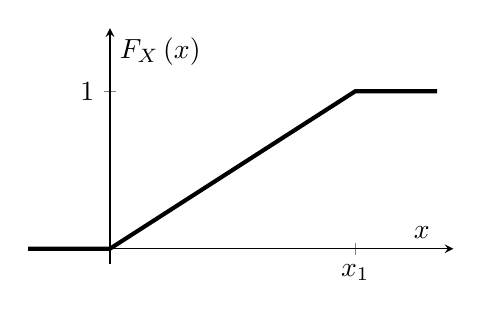
\begin{tikzpicture}
	\begin{axis}[% Cosas comunes a todos los gráficos
		width=5.4cm,height=3cm, scale only axis,
		xmin=-1, xmax=4.2, xlabel={$x$},xtick={0,3},xticklabels={,$x_{1}$,},
		ymin=-0.1, ymax=1.4, ytick={1},
		axis x line=middle,
		x tick label style={{xshift=0pt},{yshift=0pt}}, ylabel=$F_{X}\left( {x} \right)$,yticklabels={$1$},
		x label style={{xshift=-5pt},{yshift=0pt}},
		axis y line=middle]
	 	\draw[line width=1.5pt, color=black] (axis cs:-1,0) --(axis cs:0,0) --  (axis cs:3,1) --  (axis cs:4,1);
	\end{axis}
\end{tikzpicture}  
}% 
\hspace{10pt}% 
\subfloat[][]{% 
\label{fig04-02b}% 
\begin{tikzpicture}
	\begin{axis}[% Cosas comunes a todos los gráficos
		width=5.4cm,height=3cm, scale only axis,
		xmin=-1, xmax=4.2, xlabel={$x$},xtick={0,3},xticklabels={,$x_{1}$},
		ymin=-0.1, ymax=1.4, ytick={1},
		axis x line=middle,
		x tick label style={{xshift=0pt},{yshift=0pt}}, ylabel=$f\xb{X}\left( {x} \right)$,yticklabels={$\dfrac{1}{x_{1}}$},
		x label style={{xshift=-5pt},{yshift=0pt}},
		axis y line=middle]
		\draw[line width=1.5pt, color=black] (axis cs:0,1) -- (axis cs:3,1)-- (axis cs:3,0);  
\end{axis}
\end{tikzpicture}  
}
\caption[Función de distribución y Función densidad de probabilidad de una variable aleatoria continua]{Función de distribución y Función densidad de probabilidad de una variable aleatoria continua.}
\label{fig04-02} 
\end{figure} 

Un ejemplo de cómo se gestionan las tablas que puedan segmentarse a través de más de una página se muestra en la \autoref{tab01-08}, obtenida con el siguiente código:
%
\begin{lstlisting}[frame=none]
\begin{longtable}{p{3.5cm}p{8cm}}
\caption{Funciones de manipulación de gráficos} \label{tab01-08}\\
\hline
{\rule[-8pt]{0pt}{22pt}\bfseries{Función}} & Significado\\
\hline %\rule{0pt}{1pt}
\endfirsthead
\caption[]{..continuación} \\
\hline
{\rule[-8pt]{0pt}{22pt}\bfseries{Función}} & Significado\\
\hline %\rule{0pt}{1pt}
\endhead
\hline
\endfoot %\rule{0pt}{14pt}
\texttt{xlabel('texto')} & Etiqueta el eje \texttt{x} de la gráfica actual\\ 
\texttt{ylabel('texto')} & Etiqueta el eje \texttt{y} de la gráfica actual\\ 
\texttt{title('texto')} & Título de la gráfica actual\\ 
\texttt{text(x,y, 'texto')} & Introduce ``texto'' en la posición \texttt{(x,y)} de la gráfica actual\\ 
\texttt{legend()} & Permite definir rótulos para las distintas líneas o curvas de la gráfica\\ 
\texttt{grid} & Dibuja una rejilla. Con \texttt{grid off} desaparece la cuadrícula\\ 
\texttt{axis([xmin xmax ymin ymax])} & Fija los valores máximos y mínimos de los ejes\\ 
\texttt{axis equal} &Establece que la escala de los ejes sea la misma\\ 
\texttt{axis square} & Fija que la gráfica sea un cuadrado\\ 
\end{longtable}
\end{lstlisting}
%
%
\begin{longtable}{p{3.5cm}p{8cm}}
\caption{Funciones de manipulación de gráficos} \label{tab01-08}\\
\hline
{\rule[-8pt]{0pt}{22pt}\bfseries{Función}} & Significado\\
\hline %\rule{0pt}{1pt}
\endfirsthead
\caption[]{..continuación} \\
\hline
{\rule[-8pt]{0pt}{22pt}\bfseries{Función}} & Significado\\
\hline %\rule{0pt}{1pt}
\endhead
\hline
\endfoot %\rule{0pt}{14pt}
\texttt{xlabel('texto')} & Etiqueta el eje \texttt{x} de la gráfica actual\\ 
\texttt{ylabel('texto')} & Etiqueta el eje \texttt{y} de la gráfica actual\\ 
\texttt{title('texto')} & Título de la gráfica actual\\ 
\texttt{text(x,y, 'texto')} & Introduce ``texto'' en la posición \texttt{(x,y)} de la gráfica actual\\ 
\texttt{legend()} & Permite definir rótulos para las distintas líneas o curvas de la gráfica\\ 
\texttt{grid} & Dibuja una rejilla. Con \texttt{grid off} desaparece la cuadrícula\\ 
\texttt{axis([xmin xmax ymin ymax])} & Fija los valores máximos y mínimos de los ejes\\ 
\texttt{axis equal} &Establece que la escala de los ejes sea la misma\\ 
\texttt{axis square} & Fija que la gráfica sea un cuadrado\\ 
\end{longtable}

\subsection{Gestión de índices alfabéticos y glosario}
Para gestionar el índice alfabético se ha utilizado el paquete \ttcolorc{imakeidx}\index{imakeidx}. Se ha optado por generar un índice alfabético con tres columnas y con una letra antes de cada grupo de palabras del índice. Para ello se ha redefinido el entorno \ttcolor{theindex}\index{theindex}.

Para incluir algo en el índice el comando standard es \ttcolorc{index} y además se han creado un par de comandos: el comando \ttcolorc{indexit} que pone la palabra correspondiente en cursiva y además se incluye en el índice y \ttcolorc{ind} que es idéntica a \ttcolorc{index}.

Para los glosarios se utiliza el paquete \ttcolor{glossaries}\index{glossaries} cuyo uso ya ha sido explicado.

\subsection{Ajustes en fórmulas}
La escritura de fórmulas en \LaTeX\ requiere el conocimiento de un conjunto de comandos que se encuentran muy bien explicados en el documento \ttcolor{mathmode.pdf}. Uno de los comandos que facilitan esta escritura y algunos efectos especiales se basan en el uso de los paquetes \ttcolor{cancel}\index{cancel} y \ttcolor{kbordermatrix}\index{kbordermatrix}. Para permitir la escritura de matrices con diferentes limitadores, hemos utilizado el paquete \ttcolor{array}\index{array}.

Debido a un bug de  \LuaLaTeX\ es necesario escribir fórmulas demasiado anchas mediante el entorno \comando{begin\{equationw\}}\index{equationw}. Un ejemplo se muestra a continuación y el resultado del mismo posteriormente.

\begin{LTXexample}[pos=b, hsep=15pt,width=\textwidth]
\begin{equationw}
\E\left[ {Y} \right]=\E\left[ {\left( {X-m_{X}} \right)^{n}} \right]=\begin{cases}
1\times 3 \times \cdots \times \left( {2k-1} \right)\sigma_{X}^{2k}=\frac{\left( {2k} \right)!\sigma_{X}^{2k}}{2^{k}k!}&\textrm{ para }n=2k \\
0 &\textrm{ para }n=2k +1
\end{cases}
\end{equationw}
\end{LTXexample}
Podemos observar la posición del número de ecuación que se ha desplazado debajo de la fórmula. Para crear el entorno que ha permitido resolver este error (el número de ecuación se desplazaba a la derecha), ha sido necesario cargar el paquete \ttcolor{environ}.

También para corregir otro bug de \LuaLaTeX\ hemos introducido el comando \ttcolorc{sqrtlua}\index{sqrtlua} que evita el desplazamiento del contenido bajo el signo de la raíz cuando dicho contenido tiene una altura superior a un renglón. Esta definición hay que encontrarla en el bloque de gestión de fuentes.

\subsection{Hiperenlaces}\index{hyperref}

La creación de los hiperenlaces en los documentos escritos en \LaTeX\ se gestiona mediante el paquete \ttcolor{hyperref}. La documentación de este paquete es extensa y muy detallada y permite, por ejemplo, manejar con facilidad los colores de los hiperenlaces, la utilización de comandos inteligentes como \ttcolorc{autoref}\index{autores}, etc. 

El ajuste más genérico de \ttcolor{hyperref} se ha realizado en esta hoja de estilo pero adicionalmente se han definido otros ajustes en el fichero principal de manera que, por ejemplo, se generen ficheros pdf con palabras claves que les permitan ser localizados con los buscadores, como podemos ver en la líneas de código siguientes:

\begin{lstlisting}[frame=none]
\hypersetup
	{
 	linkcolor=black, %Tocar para poner color en enlaces
	pdfauthor={\elautor},
	pdftitle={\eltitulo}, 
	citecolor=black, %Tocar para poner color en enlaces, eg blue
	pdfkeywords={Formato de Libro para la ETSI, Universidad de Sevilla}	
	 }
\end{lstlisting}
  
Dentro de este apartado, mencionar la utilización de los paquetes \ttcolor{zref-lastpage} y \ttcolor{zref-user}\index{zref-lastpage}\index{zref-user} para detectar el número total de páginas de un documento, que viene dado por \comandos{zpageref}{Lastpage}, o bien el ajuste que se realiza sobre las direcciones url, del paquete \ttcolor{url}\index{url}, que ha sido cargado automáticamente.

\subsection{Listado de códigos}
Es habitual en textos escritos en la Escuela el uso de listados de códigos de muy diversa índole. Nosotros hemos elegido el paquete \ttcolor{listings}\index{listings} para gestionarlos en nuestros documentos. Este paquete se encuentra perfectamente documentado, lo que nos ha permitido realizar algunos ajustes que hemos considerado necesarios. 

En el caso de utilizar \LaTeX\ es necesario que los símbolos no habituales se declaren, como hemos hecho en el siguiente bloque:
\begin{lstlisting}[frame=none]
\ifluatex
\else
\lstset{literate=%
    {á}{{\'a}}1
    {é}{{\'e}}1
    {í}{{\'i}}1
    {ó}{{\'o}}1
    {ú}{{\'u}}1
    {Á}{{\'A}}1
    {É}{{\'E}}1
    {Í}{{\'I}}1
    {Ó}{{\'O}}1
    {Ú}{{\'U}}1
    {ñ}{{\~{n}}}1
    {º}{{\textsuperscript{\b{o}}}}1
    {ª}{{\textsuperscript{\b{a}}}}1
    {¿}{{?`}}1
}
\fi
\end{lstlisting}
%
Y también hemos tenido que ajustar determinados problemas relacionados con el uso de los idiomas español e inglés.  Por último, hemos ajustado el ``caption'' de los códigos mediante la declaración de un formato y modificado ligeramente la manera en la que se realiza el listado de los mismos, mediante el siguiente conjunto de instrucciones.
 
\begin{lstlisting}[frame=none]
\makeatletter
	\renewcommand*{\l@lstlisting}[2]{\@dottedtocline{1}{.1em}{2.8em}{\tocsecc #1}{\tocsecc #2}}
\makeatother
\end{lstlisting}

\subsection{Entornos, teoremas y similares}
En este apartado hemos agrupado un conjunto de paquetes relacionados con la creación de entornos específicos y estructuras como los teoremas y elementos similares.

En primer lugar, utilizamos el paquete \ttcolor{mdframed}\index{mdframed} para poder crear cajas sombreadas que se continúan a través de más de una página. Aunque no se ha utilizado en este estilo, merece señalarse la existencia del paquete \ttcolor{tcolorbox}\index{tcolorbox} que permite una gestión probablemente más flexible con este mismo fin.

A continuación, señalamos la creación del entorno \ttcolor{Resumen} que permite realizar resúmenes en el lugar del texto que nos interese, como ya hemos mencionado y mostrado en un apartado anterior.

Para la gestión de los teoremas y elementos similares hemos escogido el paquete \ttcolor{ntheorem}\index{ntheorem} junto con una serie de opciones. Si analizamos las siguientes líneas de código, en la que se define el entorno \ttcolor{teor}:

\begin{lstlisting}[frame=none, numbers=left, xleftmargin=2em]
\theoremnumbering{arabic}
\theoremheaderfont{\aheadteoremas}
\theoremseparator{\hspace{.2em}}
\theorembodyfont{\itshape}
\newtheorem{teor}{\theoremname}[section]
\end{lstlisting}

Podemos observar que el la línea \ttcolor{1} el esquema de numeración será arábico, esto es, mediante números. Para su declaración utilizaremos el comando \comando{aheadteoremas} que habíamos definido anteriormente y nos indica que utilizaremos una determinada fuente con las características que habíamos señalado. El enunciado del teorema irá en \emph{cursiva} y el nombre que usaremos viene marcado por el macro  \comando{theoremname}. Por último, al incluir el término \ttcolor{section} en la línea \ttcolor{5} estamos señalando que la numeración de los teoremas se realizará al nivel de sección; esto es, las siguientes líneas de código, en las que también hemos utilizado el entorno \ttcolor{demo}, generan el teorema debajo de las mismas.

%\begin{LTXexample}[pos=b, hsep=15pt,width=\textwidth]
\begin{lstlisting}[frame=none]
\begin{teor}\label{th04-02} Si una función $f\left( {x} \right)$ tiene una segunda derivada que es no negativa (positiva) en un intervalo dado, la función es convexa (estrictamente convexa) en ese intervalo.
\end{teor}
\begin{demo} Para probar el teorema, desarrollemos la función en serie de Taylor alrededor del punto $x_{0}$:
\begin{equation}\label{eq04-321}
f\left( {x} \right)=f\left( {x_{0}} \right)+f^{\prime}\left( {x_{0}} \right)\left( {x-x_{0}} \right)+\frac{f^{\prime \prime}\left( {x^{\ast}} \right)}{2}\left( {x-x_{0}} \right)^{2}
\end{equation}
donde $x^{\ast}$ está entre $x_{0}$ y $x$. Por hipótesis, $f^{\prime \prime}\left( {x^{\ast}} \right)\ge 0$, así que el último término es no negativo para todo $x$.

...
\end{demo}
\end{lstlisting}
%\end{LTXexample}

\begin{teor}\label{th04-02} Si una función $f\left( {x} \right)$ tiene una segunda derivada que es no negativa (positiva) en un intervalo dado, la función es convexa (estrictamente convexa) en ese intervalo.
\end{teor}
\begin{demo} Para probar el teorema, desarrollemos la función en serie de Taylor alrededor del punto $x_{0}$:
\begin{equation}\label{eq04-321}
f\left( {x} \right)=f\left( {x_{0}} \right)+f^{\prime}\left( {x_{0}} \right)\left( {x-x_{0}} \right)+\frac{f^{\prime \prime}\left( {x^{\ast}} \right)}{2}\left( {x-x_{0}} \right)^{2}
\end{equation}
donde $x^{\ast}$ está entre $x_{0}$ y $x$. Por hipótesis, $f^{\prime \prime}\left( {x^{\ast}} \right)\ge 0$, así que el último término es no negativo para todo $x$.

...
\end{demo}

Existen un conjunto de entornos definidos de manera análoga al anterior y su uso puede ser fácilmente deducible del ejemplo anterior.

\subsection{Otros comandos}
Finalizamos la descripción del fichero señalando la existencia de un grupo de comandos muchos de ellos únicamente utilizables en la escritura de un texto como el presente. Otros, como las definiciones de las cabeceras de los exámenes o el que nos permite crear una dedicatoria de nuestro texto. Ambos se gestionan en el fichero principal con líneas de código similares a las siguientes:

\begin{lstlisting}[frame=none]
\dedicatoria{A nuestras familias\\A nuestros maestros} 
\titulacion{ Grado en Ingeniería de Tecnología de Telecomunicación}
\asignatura{Comunicaciones Digitales}
\convocatoria{Primera convocatoria. Curso 2013-14}
\fecha{3/02/2014}
\end{lstlisting}
%
con el resultado que ya hemos mostrado.

\section{A modo de conclusión}
Hemos tratado de mostrar en este capítulo los elementos más destacados del diseño de la hoja de estilo que hemos realizado para nuestra Escuela. Como hemos dicho con anterioridad, hay mucho de gusto personal en el diseño pero también existe un considerable compromiso con tendencias actuales en la maquetación de textos científicos. 

Como todo diseño, es manifiestamente mejorable y nuestro deseo es que este capítulo permita a quien lo desee adaptarla a sus criterios. Tenemos intención de crear una página de preguntas y respuestas que permitan, con la aportación de todos, mejorar esta primera aportación a la creación de una imagen corporativa de los documentos generados en nuestra Escuela.

 




% !TEX root =../LibroTipoETSI.tex

%:Descripción del fichero de estilo de la ETSI

\chapter{Estilo tipográfico LibroETSI}\label{estilo}

\lettrine[lraise=-0.1, lines=2, loversize=0.25]{E}{n} este Capítulo se analiza el fichero de estilo \ttcolor{libroETSI.sty} en el que se han definido los diferentes elementos que constituyen el estilo tipográfico propuesto en la Escuela Técnica Superior de Ingeniería de la Universidad de Sevilla para la redacción y publicación de libros y otros tipos de documentos. 

El objetivo de este análisis es explicar detalladamente la relación entre los paquetes que se han utilizado y su reflejo en la confección del documento, para permitir, si se desea, modificar, corregir o mejorar cualquiera de los mismos por los usuarios.

Por supuesto, como ocurre en cualquier diseño, existen propuestas alternativas a las que aquí se recogen y creemos que con la exposición realizada se facilitará una mayor extensión de la utilización de \LaTeX\ por parte de todos los miembros de nuestra Escuela. 

Es importante señalar que muchas de las instrucciones del estilo \emph{tienen que estar en el orden que se proponen}. Al ser \LaTeX\ un lenguaje en el que numerosos bloques de código (paquetes) se cargan consecutivamente, es importante el orden en el que se realiza esta carga, para evitar posibles incompatibilidades.

\section{Bloque 0}

Está formado por un conjunto de sentencias genéricas en cualquier hoja de estilo de \LaTeX\ y en él se establece el formato que va a utilizarse (LaTex2e) además de definir las posibles opciones que se han incorporado al estilo y procesarlas. Debemos observar que estas opciones pueden venir definidas o bien en la declaración del documento, como se propone en el fichero \ttcolor{libroTipoETSI.tex} o bien en la propia llamada del paquete. Así, se podrían haber escrito las primeras instrucciones del fichero \ttcolor{libroTipoETSI.tex} en la forma:

\begin{lstlisting}[rulecolor=\color{white}]
\documentclass[paper=a4,10pt, twoside]{scrbook}
\usepackage[Myfinal=true, Minion=false]{libroETSI}
\end{lstlisting}

Para poder utilizar estas opciones y alguna otra que veremos interesante introducir, como el idioma, debemos saber que, por defecto, son falsas por lo que, en realidad, no hubiera sido necesaria colocar la opción \ttcolor{Minion=false}. Sin embargo, a veces se prefiere su declaración para hacer más explícita que se está utilizando. Observar la forma que se definen las opciones mediante las instrucciones

\begin{lstlisting}[rulecolor=\color{white}]
\DeclareBoolOption{Myfinal}
\DeclareBoolOption{Minion}
\DeclareBoolOption{English}
\end{lstlisting}

\section{Bloque 1: Aspectos generales}

El primer paquete que se carga se denomina \ttcolor{etoolbox}. \index{etoolbox}Este paquete general permite importantes correcciones en el resto de la hoja de estilo, modificando de manera sustancial el comportamiento de algunos de los elementos utilizados. Así, por ejemplo, hemos utilizado un comando definido en este paquete, \ttcolor{appto} \index{appto}en la sentencia

\begin{lstlisting}[rulecolor=\color{white}]
\appto{\appendices}{\def\Hy@chapapp{Appendix}}
\end{lstlisting}
que ha resuelto un grave problema que aparece al generar el índice de un documento que tenga apéndices que esté escrito en español o cualquier otro idioma que tenga caracteres no comprendidos entre los primeros 128 del código ASCII.

A continuación se cargan un conjunto de paquetes que resuelven incompatibilidades con el tipo de documento que estamos utilizando, resuelven problemas internos o nos permiten realizar comparaciones booleanas. 

Seguidamente se carga el paquete \ttcolor{microtype}\index{microtype}, si el parámetro \ttcolor{Myfinal} es \ttcolor{true}. Este paquete es responsable de finísimos microajustes en los textos generados por \LaTeX\, permitiendo la expansión o comprensión de caracteres y espacios en blanco de un documento para mejorar su apariencia. Con diferencia a lo que se realiza en Word, \TeX\ gestiona estas correcciones a nivel de parágrafo, lo que confiere un aspecto altamente profesional a los documentos generados. Debido a la complejidad de los algoritmos que se utilizan, al cargar \ttcolor{microtype} se enlentece considerablemente la compilación del documento, por lo que resulta conveniente definir \ttcolor{Myfinal} como \ttcolor{true} únicamente en las etapas últimas de redacción. ¡Pero no sólo en la última!, puesto que el ajuste que introduce hace que a veces cambie la situación de las líneas huérfanas y viudas, de considerable importancia desde un punto de vista tipográfico. 

Siguiendo los consejos de los editores de IEEE, se han modificado un conjunto de valores por defecto lo que hace el documento menos restrictivo en lo referente a la colocación de los elementos flotantes dentro de una página. Además, se ha optado por permitir que un conjunto de fórmulas que constituyan un bloque (definidas dentro del entorno  \comandos{begin}{align}... \comandos{end}{align}, por ejemplo) puedan escribirse en diferentes páginas. Si se desea cambiar este comportamiento, simplemente debemos modificar el valor de \ttcolorc{interdisplaylinepenalty} a un valor más elevado, por ejemplo $10000$.

Aunque el tipo de documento utilizado, \ttcolor{scrbook}\index{scrbook}, incorpora por defecto un conjunto de instrucciones que permiten una gestión muy eficiente del tamaño de los diferentes elementos que constituyen una página (cabecera, ancho del texto, altura, pie de página, offset de encuadernación, etc, ) se ha optado por utilizar el paquete \ttcolor{geometry}\index{geometry} para ese fin. En el fichero de estilo simplemente se carga el paquete y los parámetros concretos se definen posteriormente en el fichero principal que estemos utilizando. Por ejemplo, este documento se ha generado con los siguientes:

\begin{lstlisting}[rulecolor=\color{white}]
paperheight=240mm,% Altura de la página
paperwidth=170mm,%   Anchura
top=25mm,%
headsep=7.5mm,%
footskip=10mm,%
textheight=190mm,%     Altura del texto
textwidth=124mm,%      Ancho del texto
bindingoffset=15mm,%   Offset de encuadernación
twoside
\end{lstlisting}

Finalizamos este bloque definiendo un alias para el tamaño básico de la fuente que hemos declarado en la sentencia inicial para poder realizar un escalado de los diferentes tamaños que se van a usar en el documento. Observad que se crean dos dimensiones, para la fuente y para el interlineado. \ttcolorc{lnormal} y \ttcolorc{lbnormal}, respectivamente.

\section{Bloque 2: Idioma, Codificación y Fuentes}
\subsection{Idioma}
La posibilidad de utilizar nuestra plantilla para escribir textos en inglés (es el único idioma aparte del español que se ha considerado) nos obliga a establecer una posible opción para cargar el paquete \ttcolor{babel}\index{babel} de una u otra manera. Este paquete es el responsable de establecer las reglas de partición silábica, entre otras cosas, por lo que resulta imprescindible su incorporación a una hoja de estilo. Cabe decir que en estos momentos el responsable de su mantenimiento es el español Javier Bezos, lo que nos garantiza una excelente adaptación del paquete a nuestro idioma.

Además de la partición silábica, un determinado conjunto de macros quedan automáticamente traducidos como por ejemplo, la definición de límite, máximos y mínimos que se utilizan en la escritura matemática. Observemos cómo aparecen unos y otros en función del idioma que utilicemos:
\begin{LTXexample}[pos=r, hsep=15pt,width=0.45\textwidth]
\begin{align*}
\lim_{n\to\infty}a_{n}&=10\\
\max\left[{a,b}\right]&=a
\end{align*}
\figurename, \tablename

\selectlanguage{english}
\begin{align*}
\lim_{n\to\infty}a_{n}&=10\\
\max\left[{a,b}\right]&=a
\end{align*}
\figurename, \tablename
\selectlanguage{spanish} 
\end{LTXexample}

El grupo de macros que gestionan los nombres que cambian en uno y otro caso, se encuentra a continuación en el fichero de estilo. 
\subsection{Codificación}
Para gestionar la forma en la que se controla la codificación en la que está escrita los ficheros fuentes de \LaTeX\ se utiliza el paquete \ttcolor{inputenc}\index{inputenc} junto con el paquete \ttcolor{fontenc}\index{fontenc}. Estos dos paquetes sólo son necesarios si no utilizamos \LuaLaTeX\ ya que en caso de utilizarse este motor, la gestión se realiza por un mecanismo completamente diferente, interno al propio motor y del que podemos despreocuparnos. 

\subsection{Fuentes del texto y comandos asociados}
La selección de la fuente a utilizar depende fundamentalmente de qué motor estemos utilizando para generar nuestro texto. Si optamos por \LaTeX\ (en realidad, pdf\LaTeX\ ), la selección del texto normal se realiza en el fichero principal mediante el comando \comandos{usepackage}{tgtermes}, que selecciona para el texto un clon de la fuente Times. En general, las fuentes que se pueden utilizar con \LaTeX\ no son demasiadas y una excelente recopilación de las disponibles se encuentra en la dirección \url{http://www.tug.dk/FontCatalogue/}. 

Sin embargo, si nuestro motor es \LuaLaTeX, podemos utilizar como fuente de texto cualquier fuente .otf ó .ttf presente en nuestro ordenador. Cómo se cargan dichas fuentes y cómo se utilizan se encuentra recogido en la documentación del paquete \ttcolor{fontspec}\index{fontspec} y en nuestro estilo se muestra en las líneas de código siguientes:
\begin{lstlisting}[rulecolor=\color{white}]
\setmainfont[Renderer=Basic, Ligatures=TeX,% 
	Scale=1.0,%
	]{Times New Roman}
\end{lstlisting}

La fuente que hemos seleccionado de esta manera es la que utilizaremos en el texto normal. Es decir, en todo el texto que no sea cabeceras de página, enunciados de secciones, captions de figuras, etc. Para todos estos casos, como una elección de diseño, hemos utilizado una fuente perteneciente al tipo denominado \emph{sin serif}. En el caso de \LaTeX\ hemos optado por una fuente {\ifluatex{\fontspec[Scale=0.95]{Helvetica}Helvética Narrow}\else{Helvética Narrow}\fi}, mientras que en el caso de \LuaLaTeX\ hemos utilizado una fuente {\ifluatex{\fontspec{Arial Narrow}Arial Narrow}\else{Arial Narrow}\fi}. Los comandos iniciales de esta decisión se muestran en las siguientes líneas de código.
\begin{lstlisting}[rulecolor=\color{white}]
\ifluatex
	\setsansfont[Ligatures=TeX,		% Se puede obtener un texto sin serif con \ssfamily				
	Scale=0.95,
	]{Arial Narrow}
\else
	\renewcommand{\sfdefault}{phv} 
\fi
\end{lstlisting}

Podemos observar la sintaxis completamente diferente que se utiliza en un caso y otro.  En realidad, para facilitar la utilización de diversas variantes de ambas fuentes, en cualquiera de los dos motores de composición elegidos, hemos definido un conjunto de comandos que están recogidos en las siguientes líneas.

\begin{lstlisting}[rulecolor=\color{white}]
\ifluatex

	\newfontfamily\helveticam{Arial}						% Helvética
	\newfontfamily\helveticab{Arial Bold}					% Helvética Bold
	\newfontfamily\helveticai{Arial Italic}					% Helvética itálica
	\newfontfamily\helveticax{Arial Bold Italic}				% Helvética Bold Itálica

	\newfontfamily\titular{ArialNarrow-Bold}				% Para los titulares
	\newfontfamily\titulart{ArialNarrow-Bold}				% Para los titulos
	\newfontfamily\titulari{ArialNarrow-BoldItalic}			% Para los titulares oblicua

	\newfontfamily\titulartoc{ArialNarrow}					% Para el TOC
	\newfontfamily\titulartocb{ArialNarrow-Bold}			% Para el TOC bold
	\newfontfamily\titulartoci{ArialNarrow-BoldItalic}		% Para el TOC oblicua

\else

	\newcommand{\helveticam}{\usefont{T1}{phv}{m}{n}\selectfont }
	\newcommand{\helveticab}{\usefont{T1}{phv}{b}{n}\selectfont }
	\newcommand{\helveticai}{\usefont{T1}{phv}{m}{it}\selectfont }
	\newcommand{\helveticax}{\usefont{T1}{phv}{b}{it}\selectfont }

	\newcommand{\titular}{\usefont{T1}{phv}{bc}{n}\selectfont }
	\newcommand{\titulari}{\usefont{T1}{phv}{bc}{it}\selectfont }
	\newcommand{\titulart}{\usefont{T1}{phv}{bc}{n}\selectfont }
	
	\newcommand{\titulartoc}{\usefont{T1}{phv}{mc}{n}\selectfont }
	\newcommand{\titulartocb}{\usefont{T1}{phv}{bc}{n}\selectfont }
	\newcommand{\titulartoci}{\usefont{T1}{phv}{mc}{it}\selectfont }
	
\fi
\end{lstlisting}

De esta manera para el usuario del paquete es transparente el uso de \LaTeX\ o \LuaLaTeX . La sintaxis en este último caso se debe a la utilización del paquete \ttcolorc{usepackage[no-math]\{fontspec\}} que hemos cargado con anterioridad y en el caso de \LaTeX\ al uso de instrucciones básicas del esquema de selección de fuentes.

En cualquier caso, hasta este momento sólo hemos definido los comandos que nos permitirán hacer uso de las tipografías seleccionadas. Su aplicación concreta, con el tamaño que hemos elegido debe realizarse a continuación. En primer lugar, para facilitar un escalado adecuado de las distintas fuentes, hemos definido un conjunto de dimensiones relativas como, por ejemplo,
\begin{lstlisting}[frame=none]
\newdimen\lcatorce
\newdimen\lbcatorce
\end{lstlisting}
y posteriormente le hemos asignado valores, 
\begin{lstlisting}[frame=none]
\lcatorce=\dimexpr1.4\dimexpr\lnormal
\lbcatorce=\dimexpr1.4\dimexpr\lbnormal
\end{lstlisting}

Estos valores se corresponden  en este caso a fracciones (1,4 ó 140\%) del tamaño de la fuente normal que, recordemos, habíamos definido con anterioridad.

Por último, un conjunto de comandos facilita la utilización de las fuentes en sus diversas variaciones a lo largo de todo el texto. Así, por ejemplo, se ha definido en la siguiente línea de código un comando para definir la fuente y el tamaño que vamos a usar en los títulos de las secciones:
\begin{lstlisting}[frame=none]
\newcommand{\aheadsecc}{\fontsize{\ltrece}{\lbtrece} \titular}
\end{lstlisting}

Por supuesto, una vez que hemos definido este comando, podemos utilizarlo siempre que deseemos. Así, la utilización y el resultado del comando \ttcolorc{aheadsecc} se muestra a continuación:
\begin{LTXexample}[pos=r, hsep=15pt,width=0.45\textwidth]
\aheadsecc{Como si fuera una sección}
\end{LTXexample}

\subsection{Fuentes matemáticas y símbolos}
En una Escuela de Ingeniería la gestión de las fuentes matemáticas en nuestros documentos juega un papel fundamental. Po ello, si utilizamos \LuaLaTeX\ es necesario cargar los paquetes \ttcolor{lualatex-math}\index{lualatex-math} y \ttcolor{luatextra}\index{luatextra}. Observar además que aparte de estos dos paquetes, orientados básicamente a la utilización de aspectos concretos relacionados con símbolos matemáticos, hemos incluido el comando \ttcolorc{usepackage[no-math]\{fontspec\}}. Aunque \ttcolor{fontspec} se utilizará en la gestión del tipo de fuentes y comandos relacionados con las mismas, es necesario incluirlo aquí por el típico problema que hemos mencionado anteriormente del orden en el que se encargan los paquetes.

En general, para mejorar el escalado de determinados símbolos, utilizaremos el paquete \ttcolor{exscale}\index{exscale}. Advertimos nuevamente que \emph{se tiene que cargar exactamente antes que el paquete \ttcolor{amsmath}\index{amsmath}}, que se carga a continuación, junto con una adición recomendable, el paquete \ttcolor{mathtools}\index{mathtools}.

Existen numerosos paquetes que definen los símbolos matemáticos más habituales. Uno de los más completos es el paquete \ttcolor{MnSymbol}\index{MnSymbol}, especialmente indicado cuando la fuente del texto es la Minion, licenciada por Adobe. Sin embargo, la utilización tanto de la fuente de símbolos como la fuente de texto dentro de \LaTeX\ es un asunto no trivial. Requiere la disponibilidad de la fuente Minion, y la creación del  paquete \ttcolor{MinionPro}\index{MinionPro}. El lector interesado puede encontrar el procedimiento para crear dicho paquete en \url{https://github.com/sebschub/FontPro/}.

Si se han seguido las instrucciones que se encuentran en la dirección anterior y se desea utilizan la fuente, se indicará mediante uno de las opciones del programa, escribiendo \ttcolor{Minion=true}. Con ello, se cargarían los correspondientes paquetes mediante las primeras líneas del siguiente código:
\begin{lstlisting}[rulecolor=\color{white}]
\makeatletter
\ifdtsc@Minion
	\usepackage{MnSymbol}
	\usepackage[mathlf, minionint, mnsy]{MinionPro}
	\newcommand{\bm}{\ensuremath{\boldsymbol}}
\else
	\usepackage{amssymb}
	\usepackage{mathptmx}
	\usepackage{amsfonts}
	\usepackage{bm}
\fi
\makeatother
\end{lstlisting}

En el caso que no se tenga instalado el paquete, o no se desee utilizar, basta ignorar la opción y se ejecutarán las restantes líneas del código anterior. 

\section{Bloque 3: Tabla de contenidos}
Uno de los aspectos sobresalientes de \LaTeX\ es la facilidad para generar la \emph{Tabla de contenidos} (TOC) de un documento. No sólo para generarla sino también para controlar cómo se presenta y cómo se gestiona el contenido de la misma. En esta sección explicaremos los comandos que hemos utilizado con este fin, teniendo en cuenta que hemos actuado directamente renombrado y creando nuevos elementos, sin utilizar paquetes específicos para esta tarea. Si alguno desea hacer uso de los mismos, unos de los más ampliamente utilizados es el paquete \ttcolorc{tocloft}\index{tocloft}.

Para controlar dónde queremos que aparezca la tabla de contenido, debemos utilizar el comando \ttcolorc{tableofcontens}\index{tableofcontens}. Si analizamos el fichero principal de este documento, veremos que precediendo a este comando aparecen las líneas
\begin{lstlisting}[frame=none]
\cleardoublepage
\phantomsection
\addcontentsline{toc}{listasf}{Índice}
\pagestyle{especial}
\end{lstlisting}
Con ellas indicamos, en primer lugar, que la tabla de contenidos siempre va a aparecer en una página impar, que haremos uso de un estilo de página\footnote{Más adelante veremos cómo se definen estos estilos.} que denominamos \ttcolor{especial} y que queremos que la propia tabla de contenido (o índice del documento) aparezca referenciada en en el índice, aunque pueda parecer complejo entender lo que esto significa.\LaTeX\ permite controlar el nombre que le hemos asignado a la tabla de contenido mediante la sentencia \comando{def}\comando{contentsname}\ttcolor{\{Índice\}}, tal como se define en otro lugar del estilo, puesto que este nombre dependerá del idioma que utilicemos.
 
A la hora de construir esta tabla de contenidos, nuestra primera decisión fue establecer que iban a aparecer hasta los apartados que hemos denominados \ttcolor{subsubsecciones}, lo que se logra mediante el \ttcolor{\{3\}} del comando \comandos{setcounter}{tocdepth}\index{tocdepth} en \ttcolor{libroETSI.sty}.  Cambiar este número haría aparecer menos apartados o más, dependiendo de la elección.

Para establecer la manera en la que cada nivel de segmentación aparece en el TOC hacemos uso de una secuencia de comandos similares a las mostradas a continuación para el caso del capítulo:
\begin{lstlisting}[frame=none, numbers=left, xleftmargin=2em]
\makeatletter
	\renewcommand*\l@chapter[2]
	{
    \addpenalty{-\@highpenalty}%
    \vskip 0.5em \@plus\p@
	 \@dottedtocline{0}{0em}{1em}{\tocchap #1}{\tocchap #2}
	}
\makeatother
\end{lstlisting}
El elemento clave está recogido en la línea \ttcolor{6}. El significado de cada uno de los parámetros es el siguiente: el \ttcolor{0} señala que estamos formateando el nivel de capítulo. El siguiente parámetro, \ttcolor{0em} establece la indetación de la línea, \ttcolor{1em} define la anchura que reservamos para el número que mostramos, si es que la parte tiene números y los otros dos establecen las características tipográficas que vamos a utilizar para el título (incluyendo el número si lo hubiera) y el número de la página en el que se encuentra la correspondiente parte. Este ajuste se ha realizado sin tener en cuenta ninguno de los paquetes, únicamente utilizando sentencias del propio núcleo de \LaTeX\. De forma similar hemos procedido para el resto de los elementos de segmentación del texto.

Aunque algo redundante, nuestra siguiente decisión afecta a la manera en la que hemos querido que aparezcan en el índice los índices del texto (valga la redundancia), tales como el \emph{Índice de Figuras}, \emph{Índice Alfabético}, etc y otros elementos como el \emph{Resumen, Prefacio}, etc o la \emph{Bibliografía}. No es trivial pero, básicamente, hemos definido dos listas, una para los elementos que aparecen antes del Índice y otra para los  que aparecen después, al final del texto, que se corresponden aproximadamente a lo que hemos denominado \ttcolorc{frontmatter}\index{frontmatter} y \ttcolorc{backmatter}\index{backmatter}, respectivamente. Si nos fijamos por ejemplo en la lista que hemos denominado \ttcolorc{listasf}, cómo se representan los elementos que están incluidos en la misma se realiza con las instrucciones
\begin{lstlisting}[frame=none]
\makeatletter
	\newcommand*\l@listasf[2]
	{
    \addpenalty{-\@highpenalty}%
    \vskip 0.05em \@plus\p@
	 \@dottedtocline{0}{0em}{2.5em}{\fontsize{\lnueve}{\lbnueve}\selectfont \helveticai #1}{\fontsize{\lnueve}{\lbnueve}\titulartoc #2}
	}
\makeatother
\end{lstlisting}
en las que vemos, por ejemplo, que el tamaño del texto es el tamaño relativo \ttcolorc{lbnueve}, junto con una fuente \ttcolorc{helveticai} represente esta fuente lo que represente (en un apartado anterior ha quedado definido).

Una cuestión distinta es las instrucciones que debemos ejecutar para incluir un determinado elemento en la lista correspondiente. Por ejemplo, para incluir el \emph{Prefacio} en la  \ttcolorc{listasf}, observemos que hemos escrito el siguiente comando: 
\begin{lstlisting}[frame=none]
\addcontentsline{toc}{listasf}{Prefacio}
\end{lstlisting}

Para finalizar este apartado, también hemos propuesto que no aparezcan los habituales puntos que existen entre el texto y el número de página correspondiente de muchos índices, ajustando a \ttcolor{10000} el parámetro \ttcolor{\textbackslash@dotsep}. Unas referencias interesantes para manejar todos estos elementos las encontramos en las siguientes direcciones \url{http://tex.stackexchange.com/questions/110253/what-the-first-argument-for-lsubsection-actually-is} y \url{http://tex.stackexchange.com/questions/33841/how-to-modify-the-indentation-before-sectioning-titles-in-the-table-of-contents}.

\section{Bloque 4: Estilos de Páginas y Títulos}
Este apartado ha sido uno de los más complejos en cuanto a diseño se refiere, atendiendo a la gran cantidad de elementos que componen un texto y sus interrelaciones. 

En general, se recomienda que los tipos de páginas diferentes que se utilicen en un documento sea un número muy limitado. Por ello, \LaTeX\ no establece un mecanismo elemental para definir distintos tipos de páginas (en realidad, únicamente un tipo \ttcolor{plain} y un tipo \ttcolor{empty}) y debemos acudir a paquetes específicos que nos permitan una mayor libertad de diseño. Lo mismo podríamos decir a la hora de definir el formato de los distintos elementos, lo que hemos denominado genéricamente \emph{Títulos}, haciendo con ello referencia a los \emph{Títulos} de los capítulos, secciones, subsecciones, etc. 

Hemos de tener en cuenta que el aspecto de un libro está básicamente determinado por el formato que se ha elegido para los diferentes títulos de las partes que lo constituyen, el formato de las páginas y qué queremos que aparezca en las cabeceras y pies de páginas del mismo. Todo esto se ha conseguido utilizando un paquete desarrollado por el español Bezos denominado \ttcolor{titlesec}\index{titlesec}, que se carga en nuestro fichero mediante la instrucción \comandos{usepackage[noindentafter, pagestyles,...]}{titlesec}. En el listado siguiente se recogen algunos de los elementos de los formatos elegidos para que mediante su análisis podamos realizar nuestro propio diseño.
\begin{lstlisting}[frame=none, numbers=left, xleftmargin=2.5em]
\newpagestyle{esitscCD}
	{
	\esirulehead
	\sethead[\numpagpar \rhfont\chaptername\ \thechapter. \;\chaptertitle][][]%
			{}{}{\rhfont\thesection\ \;\sectiontitle \numpagodd}
	}

\newpagestyle{primera}
	{
	\esirulehead \footrule
  	\sethead[][][]{\includegraphics[width=2 cm]{logoUS.pdf}}%
  				{\raisebox{0.8cm}{\begin{minipage}{0.515\textwidth}
				\centering
				{\aheadsubsecc \fromtitulacion}\\
				\vspace*{.5ex}
				{\normalfont \fromasignatura}\\
				\vspace*{1ex}
				\normalfont \fromconvocatoria \quad \fromfecha
				\end{minipage}}
				}%
				{\includegraphics[width=4 cm]{logoTSC.pdf}
				}
	\setfoot{}{\rhpagefont Pág. \thepage\, de\, \zpageref{LastPage}}{}
  	}

\newpagestyle{examen}
	{
	\esirulehead
	\sethead[\rhpagefont Pág. \thepage\, de\, \zpageref{LastPage}][\aheadsubsecc\fromasignatura][[\rhpagefont\fromfecha]%
	{[\rhpagefont\fromfecha}{\aheadsubsecc\fromasignatura}{\rhpagefont Pág. \thepage\, de\, \zpageref{LastPage}}
	}

\newpagestyle{problema}
	{
	\esirulehead
    	\sethead[\numpagpar][][\rhfont\chaptername \; \thechapter. \chaptertitle]% even
        		{\rhfont\theproblema \; \problematitle}{}{\numpagodd}% odd
    	}
\newpagestyle{especial}
	{ 
	\esirulehead
	\sethead[\numpagpar][\rhfont\chaptertitle][] {}{\rhfont\chaptertitle}{\numpagodd}
	}

\newpagestyle{paginablanco}
	{
  	\sethead[][][]{}{}{}
	    \vspace*{0.2\textheight}
    \begin{center}
    {\emph{Página en blanco} }
    \end{center}
	}
	
\renewpagestyle{plain}
{
\setfoot[][\rhpagefont\thepage][]{}{\rhpagefont\thepage}{}
}
          
%:Estilo de capítulos con numeración
\titleformat{\chapter}{\vspace{75pt}\achapnum} {\makebox[25 pt]{\raggedright\thechapter}}{8pt}{\hspace*{-6pt}\raggedright\achaptext #1}[\vspace{0.3pc} {\color{gray!75}\titlerule[3.5pt]} \vspace{50pt}]
\titlespacing{\chapter}{0 pt}{0 pt}{0 pt}[0 pt]

%:Estilo de capítulos sin numeración
\titleformat{name=\chapter,numberless}{\vspace{75pt}}{}{0pc}{\filleft\achaptext #1}[\vspace{0.3pc} {\color{gray!75}\titlerule[3.5pt]} \vspace{50pt}]
\titlespacing{name=\chapter,numberless}{0 pt}{0 pt}{0 pt}[0 pt]

%:Estilo de sección     
\titleformat{\section}{\aheadsecc}{\thesection}{10 pt}{#1} 
\titlespacing{\section}{0 pt}{3ex plus .1ex minus .2ex}{3ex plus .1ex minus .2ex}

%:Estilo de sección sin numeración     
\titleformat{name=\section,numberless} {\aheadsecc}{}{0 pt}{#1} 
\titlespacing{name=\section,numberless}{0 pt}{3ex plus .1ex minus .2ex}{3ex plus .1ex minus .2ex}

%:Estilo de sección sin numeración personal
\titleclass{\misection}{straight}[\chapter]        
\titleformat{name=\misection,numberless}{\aheadsecc}{}{0 pt}{#1} 
\titlespacing{name=\misection,numberless}{0 pt}{3ex plus .1ex minus .2ex}{3ex plus .1ex minus .2ex}

%:Estilo de problema en un libro con capítulos de problemas   
\newcounter {problema}[chapter]
\makeatletter
\renewcommand {\theproblema}{P. \thechapter.\@arabic\c@problema}
\makeatother
\newcommand{\problemtitle}{}

\titleclass{\problema}{straight}[\chapter]  
\titleformat{name=\problema}{\aheadsecc}{\theproblema}{10 pt}{#1}[]      
\titlespacing{name=\problema}{0 pt}{3ex plus .1ex minus .2ex}{3ex plus .1ex minus .2ex}

\makeatletter
\let\problemaint\problema
\def\problema{\@ifnextchar[\problemaii\problemai}
\def\problemai#1{\gdef\problematitle{#1}\problemaint{#1}}
\def\problemaii[#1]#2{\gdef\problematitle{#1}\problemaint[#1]{#2}}
\makeatother

%:Para que el cambio del tipo de página se gestione con los comandos
\makeatletter
	\let\problema@without@pagestyle\problema
	\def\problema{\pagestyle{problema}\problema@without@pagestyle}
\makeatother

\makeatletter
	\let\section@without@pagestyle\section
	\def\section{\pagestyle{esitscCD}\section@without@pagestyle}
\makeatother
\end{lstlisting}

La definición de los estilos de páginas se realiza siguiendo el modelo que podemos ver entre las líneas \ttcolor{1} y \ttcolor{6} para el estilo de página por defecto, que hemos denominado \ttcolor{esitscCD}. En la línea \ttcolor{3} se define el comando \ttcolorc{esirulehead} que es el responsable de la línea de cabecera o bien, algún comando más para controlar el pie de página, como se puede observar en la línea \ttcolor{31} de otro de los estilos de página o cualquier comando genérico.

A continuación, mediante la sección \ttcolorc{sethead[][][]\{\}\{\}\{\}} definimos los elementos que vamos a incorporar en las secciones izquierda, centro y derecha de las páginas pares ó izquierda centro y derecha de las páginas impares. Las líneas \ttcolor{4} y \ttcolor{5} son las responsables de las cabeceras de este documento y creemos que es fácil entender su funcionamiento.

Un ejemplo diferente lo encontramos en el estilo de página \ttcolor{especial}. Podemos observar que en este caso las páginas pares e impares son las mismas diferenciándose únicamente en la posición del número de página.

El paquete permite definir con gran libertad estilos de páginas mucho más complejos, como podemos apreciar en los estilos de página que hemos denominado \ttcolor{primera} (primera página de un examen) y \ttcolor{examen}. Así, se han incluido en las cabeceras logos, varias líneas o un contador del número de páginas de las que consta el examen, como podemos ver en un ejemplo concreto en la  \autoref{fig04-01}.

\begin{figure}[htpb]
\centering 

\includegraphics[width=0.8\textwidth]{figuras/cabeceras.pdf}
\caption{Ejemplos de cabeceras de la página primera de un examen y de la página segunda}\label{fig04-01}%\vspace{-.5 cm}
\end{figure} 

Como últimos ejemplos de definición de estilos de páginas, se muestran las definiciones del estilo de página \ttcolor{paginablanco} que generaría una página en blanco, con el texto \emph{Página en blanco} en su centro, o el estilo \ttcolor{plain}, que es una modificación del estilo definido por defecto en \LaTeX.

A continuación, en el anterior código, se muestran varios ejemplos de definiciones de los elementos de segmentación del texto. El paquete \ttcolor{titlesec} es la referencia para estudiar cómo se han definido y solamente destacar que se ha creado un nuevo elemento, \ttcolorc{problema} para poder gestionar los problemas como si fueran secciones de un libro permitiendo, por ejemplo, su inclusión en la tabla de contenidos. 

Es importante prestar especial atención a las líneas de código \ttcolor{99}-\ttcolor{107}. En ella establecemos que siempre que definamos un problema o una sección, nos garantizamos que las páginas que vamos a utilizar se correspondan respectivamente con la página especial de problemas o con la página general de nuestro texto. Con ello logramos que en las cabeceras correspondientes queden reflejados el problema o la sección en la que nos encontramos. 

\section{Bloque 5: Gestión general del documento}
En este Bloque 5 se recogen un gran número de comandos, cargas de paquetes y ajustes que, como su nombre indica, permite una mejor gestión del documento.  La gran extensión del mismo, más de 700 líneas de código, hace inviable su descripción pormenorizada y nos limitaremos a señalar los elementos más importantes. Debemos insistir que el orden en el que se ejecuta la carga de los paquetes no es arbitrario y hay restricciones sobre este orden que pueden dar lugar a inconsistencias y errores. 

\subsection{Apéndices}
Para la gestión de los apéndices se ha elegido el paquete \ttcolor{appendix}. Para ajustar la manera en la que se muestran los apéndices en el texto, se modifica dentro del entorno el formato de \ttcolorc{chapter} de manera que también se incluya la palabra \emph{Apéndice} dentro de la definición del mismo. También se ha utilizado dentro del entorno una página de estilo especial y para evitar un problema con la tabla de contenidos cuando se utiliza el idioma español, ha sido necesario incluir las siguiente líneas de código:

\begin{lstlisting}[frame=none]
\makeatletter
	\appto{\appendices}{\def\Hy@chapapp{Appendix}}
\makeatother
\end{lstlisting}
%
que se encuentran situadas tras la carga del paquete \ttcolor{hyperref} para garantizar un correcto funcionamiento.

\subsection{Colores}
Entre los diversos paquetes que permiten la utilización de colores dentro de \LaTeX\ hemos elegido \ttcolor{xcolor}\index{xcolor} con las opciones \ttcolor{svgnames, x11names}. En la documentación del mismo vemos que existe una gran variedad de colores y esquemas que pueden utilizarse con mucha facilidad. Creemos que es una buena idea definir los colores en un lugar concreto y un ejemplo de cómo puede hacerse se muestra en las siguientes líneas.

\begin{lstlisting}[frame=none]
\usepackage[svgnames, x11names]{xcolor}
\definecolor{light-gray}{gray}{0.90}
\definecolor{shadecolor}{gray}{0.90}
\definecolor{refcolor}{named}{Black}
\definecolor{Matlabcolor}{RGB}{252,251,220}
\end{lstlisting}
%
También hemos definido en el fichero correspondiente a la edición colores propios de la ETSI:

\begin{lstlisting}[frame=none]
\definecolor{etsi}{RGB}{83,16,12}
\definecolor{fondo}{RGB}{136,18,1}
\definecolor{texto}{RGB}{253,181,138}
\definecolor{logoetsi}{RGB}{176,124,96}
\end{lstlisting}

\subsection{Aspectos genéricos de tratamiento del texto}
A continuación hemos cargado un conjunto de paquetes que mejoran aspectos genéricos y facilitan la utilización de logos y acentos especiales.  Por ejemplo, el paquete \ttcolor{icomma}\index{icomma} corrige un pequeño error en \LaTeX\ y establece una separación correcta de la coma decimal.

En este bloque también está incluido la asignación de un valor al contador \ttcolor{secnumdepth}\index{secnumdepth}. Con la instrucción 

\begin{lstlisting}[frame=none]
\setcounter{secnumdepth}{4}
\end{lstlisting}
%
le asignamos el valor de 4, que significa que hasta las  subsecciones deben aparecer numeradas. No debemos confundir este parámetro con  \ttcolor{tocdepth}\index{tocdepth}, que establece hasta qué nivel debe aparecer en la tabla de contenidos. 

La gestión de los subíndices y superíndices en las ecuaciones matemáticas se realiza de forma diferente según estemos compilando con \LaTeX\ o \LuaLaTeX . En este último caso, el control es muy preciso diferenciándose incluso si la ecuación está en línea con el texto o bien no lo está.

Adicionalmente hemos definido el comando \ttcolorc{xb} que permite modificar la posición de los subíndices cuando se utilizan con letras descendientes como la \emph{f} o \emph{g}. En el siguiente ejemplo se muestra su utilización (o no) y el resultado que se obtiene.
\begin{LTXexample}[pos=r, hsep=15pt,width=0.45\textwidth]
\begin{align*}
f_{1}(t)&=\sen(\omega_{0}t)\\
f\xb{1}(t)&=\sen(\omega_{0}t)\\
g_{i}(t)&=\sen(\omega_{0}t)\\
g\xb{i}(t)&=\sen(\omega_{0}t)
\end{align*}
\end{LTXexample}

También hemos creado un conjunto de comandos que facilitan la escritura de los subíndices y superíndices en modo texto, \ttcolorc{tsp} y \ttcolorc{tsb}.

Asimismo se incluyen en este apartado los paquetes ya mencionados \ttcolor{epigraph}\index{epigraph}, que permite escribir un epígrafe en el lugar que se desee y el paquete \ttcolor{lettrine}\index{lettrine}, con el que obtenemos el efecto de la primera letra del texto del capítulo en mayúscula y negrita y ocupando más de un renglón. Ambos paquetes han sufrido ajustes y en las siguientes líneas se recogen los realizados en el texto y autor del epígrafe.

\begin{lstlisting}[frame=none]
\makeatletter			%% El texto
\renewcommand{\@epitext}[1]
	{%
	\begin{minipage}{\epigraphwidth}
		\begin{\textflush} \itshape #1\\
		\ifdim\epigraphrule>\z@ \@epirule \else \vspace*{1ex} \fi
		\end{\textflush}
	\end{minipage}
	}
\makeatother

\makeatletter			%% El autor
\renewcommand{\@episource}[1]
	{%
	\begin{minipage}{\epigraphwidth}
		\begin{\sourceflush} \scshape #1\end{\sourceflush}
	\end{minipage}
	}	
\makeatother
\end{lstlisting}

\LaTeX\ ofrece la posibilidad de crear tablas de contenidos abreviadas de muy diversos tipos. Aunque en este texto no se han confeccionado, el paquete \ttcolor{shorttoc}\index{shorttoc} permite su gestión. Por último, destacar el uso del paquete \ttcolor{enumitem}\index{enumitem} para facilitar la creación de listas enumeradas.

\subsection{Elementos flotantes}

En \LaTeX\ , los elementos flotantes son las tablas y figuras y tienen un gran número de parámetros que se necesitan ajustar mediante un conjunto de paquetes seleccionados. Uno de los más importantes es el paquete \ttcolor{caption}\index{caption} que permite ajustar de manera muy preciso el texto que acompaña a estos elementos flotantes. 

De acuerdo con la documentación de \ttcolor{caption}, su carga y ajuste se ha realizado con las líneas de código que siguen:

\begin{lstlisting}[frame=none]
\usepackage{caption}[2013/02/03]
\DeclareCaptionLabelFormat{esisf}{\aheadteoremas{#1} \aheadteoremas{#2} }
\DeclareCaptionLabelSeparator{cuadratin}{\hspace*{3pt}}
\captionsetup{labelformat=esisf, textfont=normalfont, textformat=period, labelsep=cuadratin, format=hang, indention=0 cm,skip=10pt, labelformat=esisf}
\end{lstlisting}

Las declaraciones de formatos son diferentes para cada uno de los elementos flotantes. Así, por ejemplo, uno de los posibles recursos de \LaTeX\ es la inclusión en el texto de subfiguras, lo que se gestiona mediante el paquete \ttcolor{subfig} y la declaración de formato correspondiente, como podemos ver a continuación:

\begin{lstlisting}[frame=none]
\DeclareCaptionLabelFormat{subfig}{\aheadteoremas{#1} \aheadteoremas{(#2)} }
\captionsetup[subfigure]{labelformat=subfig }
\end{lstlisting}

Un ejemplo de ambos paquetes podemos apreciarlo en la \autoref{fig04-02}. La referencia a las subfiguras de la figura anterior se realiza con el código siguiente, de resultado mostrado a continuación. 

\begin{LTXexample}[pos=b, hsep=15pt,width=\textwidth]
en la \autoref{fig04-02}\sfx{fig04-02a} se muestra la función de distribución de una variable aleatoria continua y en la \autoref{fig04-02}\sfx{fig04-02b} su función densidad de probabilidad.
\end{LTXexample}
%
\begin{figure}[htpb]% 
\centering 
\subfloat[][]{% 
\label{fig04-02a}% 
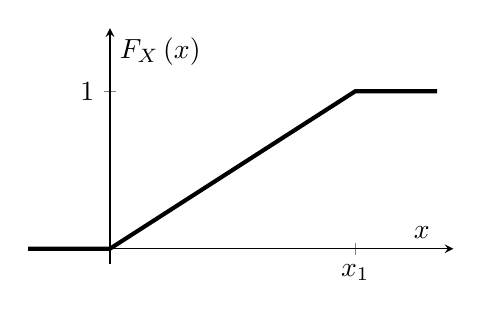
\begin{tikzpicture}
	\begin{axis}[% Cosas comunes a todos los gráficos
		width=5.4cm,height=3cm, scale only axis,
		xmin=-1, xmax=4.2, xlabel={$x$},xtick={0,3},xticklabels={,$x_{1}$,},
		ymin=-0.1, ymax=1.4, ytick={1},
		axis x line=middle,
		x tick label style={{xshift=0pt},{yshift=0pt}}, ylabel=$F_{X}\left( {x} \right)$,yticklabels={$1$},
		x label style={{xshift=-5pt},{yshift=0pt}},
		axis y line=middle]
	 	\draw[line width=1.5pt, color=black] (axis cs:-1,0) --(axis cs:0,0) --  (axis cs:3,1) --  (axis cs:4,1);
	\end{axis}
\end{tikzpicture}  
}% 
\hspace{10pt}% 
\subfloat[][]{% 
\label{fig04-02b}% 
\begin{tikzpicture}
	\begin{axis}[% Cosas comunes a todos los gráficos
		width=5.4cm,height=3cm, scale only axis,
		xmin=-1, xmax=4.2, xlabel={$x$},xtick={0,3},xticklabels={,$x_{1}$},
		ymin=-0.1, ymax=1.4, ytick={1},
		axis x line=middle,
		x tick label style={{xshift=0pt},{yshift=0pt}}, ylabel=$f\xb{X}\left( {x} \right)$,yticklabels={$\dfrac{1}{x_{1}}$},
		x label style={{xshift=-5pt},{yshift=0pt}},
		axis y line=middle]
		\draw[line width=1.5pt, color=black] (axis cs:0,1) -- (axis cs:3,1)-- (axis cs:3,0);  
\end{axis}
\end{tikzpicture}  
}
\caption[Función de distribución y Función densidad de probabilidad de una variable aleatoria continua]{Función de distribución y Función densidad de probabilidad de una variable aleatoria continua.}
\label{fig04-02} 
\end{figure} 

Un ejemplo de cómo se gestionan las tablas que puedan segmentarse a través de más de una página se muestra en la \autoref{tab01-08}, obtenida con el siguiente código:
%
\begin{lstlisting}[frame=none]
\begin{longtable}{p{3.5cm}p{8cm}}
\caption{Funciones de manipulación de gráficos} \label{tab01-08}\\
\hline
{\rule[-8pt]{0pt}{22pt}\bfseries{Función}} & Significado\\
\hline %\rule{0pt}{1pt}
\endfirsthead
\caption[]{..continuación} \\
\hline
{\rule[-8pt]{0pt}{22pt}\bfseries{Función}} & Significado\\
\hline %\rule{0pt}{1pt}
\endhead
\hline
\endfoot %\rule{0pt}{14pt}
\texttt{xlabel('texto')} & Etiqueta el eje \texttt{x} de la gráfica actual\\ 
\texttt{ylabel('texto')} & Etiqueta el eje \texttt{y} de la gráfica actual\\ 
\texttt{title('texto')} & Título de la gráfica actual\\ 
\texttt{text(x,y, 'texto')} & Introduce ``texto'' en la posición \texttt{(x,y)} de la gráfica actual\\ 
\texttt{legend()} & Permite definir rótulos para las distintas líneas o curvas de la gráfica\\ 
\texttt{grid} & Dibuja una rejilla. Con \texttt{grid off} desaparece la cuadrícula\\ 
\texttt{axis([xmin xmax ymin ymax])} & Fija los valores máximos y mínimos de los ejes\\ 
\texttt{axis equal} &Establece que la escala de los ejes sea la misma\\ 
\texttt{axis square} & Fija que la gráfica sea un cuadrado\\ 
\end{longtable}
\end{lstlisting}
%
%
\begin{longtable}{p{3.5cm}p{8cm}}
\caption{Funciones de manipulación de gráficos} \label{tab01-08}\\
\hline
{\rule[-8pt]{0pt}{22pt}\bfseries{Función}} & Significado\\
\hline %\rule{0pt}{1pt}
\endfirsthead
\caption[]{..continuación} \\
\hline
{\rule[-8pt]{0pt}{22pt}\bfseries{Función}} & Significado\\
\hline %\rule{0pt}{1pt}
\endhead
\hline
\endfoot %\rule{0pt}{14pt}
\texttt{xlabel('texto')} & Etiqueta el eje \texttt{x} de la gráfica actual\\ 
\texttt{ylabel('texto')} & Etiqueta el eje \texttt{y} de la gráfica actual\\ 
\texttt{title('texto')} & Título de la gráfica actual\\ 
\texttt{text(x,y, 'texto')} & Introduce ``texto'' en la posición \texttt{(x,y)} de la gráfica actual\\ 
\texttt{legend()} & Permite definir rótulos para las distintas líneas o curvas de la gráfica\\ 
\texttt{grid} & Dibuja una rejilla. Con \texttt{grid off} desaparece la cuadrícula\\ 
\texttt{axis([xmin xmax ymin ymax])} & Fija los valores máximos y mínimos de los ejes\\ 
\texttt{axis equal} &Establece que la escala de los ejes sea la misma\\ 
\texttt{axis square} & Fija que la gráfica sea un cuadrado\\ 
\end{longtable}

\subsection{Gestión de índices alfabéticos y glosario}
Para gestionar el índice alfabético se ha utilizado el paquete \ttcolorc{imakeidx}\index{imakeidx}. Se ha optado por generar un índice alfabético con tres columnas y con una letra antes de cada grupo de palabras del índice. Para ello se ha redefinido el entorno \ttcolor{theindex}\index{theindex}.

Para incluir algo en el índice el comando standard es \ttcolorc{index} y además se han creado un par de comandos: el comando \ttcolorc{indexit} que pone la palabra correspondiente en cursiva y además se incluye en el índice y \ttcolorc{ind} que es idéntica a \ttcolorc{index}.

Para los glosarios se utiliza el paquete \ttcolor{glossaries}\index{glossaries} cuyo uso ya ha sido explicado.

\subsection{Ajustes en fórmulas}
La escritura de fórmulas en \LaTeX\ requiere el conocimiento de un conjunto de comandos que se encuentran muy bien explicados en el documento \ttcolor{mathmode.pdf}. Uno de los comandos que facilitan esta escritura y algunos efectos especiales se basan en el uso de los paquetes \ttcolor{cancel}\index{cancel} y \ttcolor{kbordermatrix}\index{kbordermatrix}. Para permitir la escritura de matrices con diferentes limitadores, hemos utilizado el paquete \ttcolor{array}\index{array}.

Debido a un bug de  \LuaLaTeX\ es necesario escribir fórmulas demasiado anchas mediante el entorno \comando{begin\{equationw\}}\index{equationw}. Un ejemplo se muestra a continuación y el resultado del mismo posteriormente.

\begin{LTXexample}[pos=b, hsep=15pt,width=\textwidth]
\begin{equationw}
\E\left[ {Y} \right]=\E\left[ {\left( {X-m_{X}} \right)^{n}} \right]=\begin{cases}
1\times 3 \times \cdots \times \left( {2k-1} \right)\sigma_{X}^{2k}=\frac{\left( {2k} \right)!\sigma_{X}^{2k}}{2^{k}k!}&\textrm{ para }n=2k \\
0 &\textrm{ para }n=2k +1
\end{cases}
\end{equationw}
\end{LTXexample}
Podemos observar la posición del número de ecuación que se ha desplazado debajo de la fórmula. Para crear el entorno que ha permitido resolver este error (el número de ecuación se desplazaba a la derecha), ha sido necesario cargar el paquete \ttcolor{environ}.

También para corregir otro bug de \LuaLaTeX\ hemos introducido el comando \ttcolorc{sqrtlua}\index{sqrtlua} que evita el desplazamiento del contenido bajo el signo de la raíz cuando dicho contenido tiene una altura superior a un renglón. Esta definición hay que encontrarla en el bloque de gestión de fuentes.

\subsection{Hiperenlaces}\index{hyperref}

La creación de los hiperenlaces en los documentos escritos en \LaTeX\ se gestiona mediante el paquete \ttcolor{hyperref}. La documentación de este paquete es extensa y muy detallada y permite, por ejemplo, manejar con facilidad los colores de los hiperenlaces, la utilización de comandos inteligentes como \ttcolorc{autoref}\index{autores}, etc. 

El ajuste más genérico de \ttcolor{hyperref} se ha realizado en esta hoja de estilo pero adicionalmente se han definido otros ajustes en el fichero principal de manera que, por ejemplo, se generen ficheros pdf con palabras claves que les permitan ser localizados con los buscadores, como podemos ver en la líneas de código siguientes:

\begin{lstlisting}[frame=none]
\hypersetup
	{
 	linkcolor=black, %Tocar para poner color en enlaces
	pdfauthor={\elautor},
	pdftitle={\eltitulo}, 
	citecolor=black, %Tocar para poner color en enlaces, eg blue
	pdfkeywords={Formato de Libro para la ETSI, Universidad de Sevilla}	
	 }
\end{lstlisting}
  
Dentro de este apartado, mencionar la utilización de los paquetes \ttcolor{zref-lastpage} y \ttcolor{zref-user}\index{zref-lastpage}\index{zref-user} para detectar el número total de páginas de un documento, que viene dado por \comandos{zpageref}{Lastpage}, o bien el ajuste que se realiza sobre las direcciones url, del paquete \ttcolor{url}\index{url}, que ha sido cargado automáticamente.

\subsection{Listado de códigos}
Es habitual en textos escritos en la Escuela el uso de listados de códigos de muy diversa índole. Nosotros hemos elegido el paquete \ttcolor{listings}\index{listings} para gestionarlos en nuestros documentos. Este paquete se encuentra perfectamente documentado, lo que nos ha permitido realizar algunos ajustes que hemos considerado necesarios. 

En el caso de utilizar \LaTeX\ es necesario que los símbolos no habituales se declaren, como hemos hecho en el siguiente bloque:
\begin{lstlisting}[frame=none]
\ifluatex
\else
\lstset{literate=%
    {á}{{\'a}}1
    {é}{{\'e}}1
    {í}{{\'i}}1
    {ó}{{\'o}}1
    {ú}{{\'u}}1
    {Á}{{\'A}}1
    {É}{{\'E}}1
    {Í}{{\'I}}1
    {Ó}{{\'O}}1
    {Ú}{{\'U}}1
    {ñ}{{\~{n}}}1
    {º}{{\textsuperscript{\b{o}}}}1
    {ª}{{\textsuperscript{\b{a}}}}1
    {¿}{{?`}}1
}
\fi
\end{lstlisting}
%
Y también hemos tenido que ajustar determinados problemas relacionados con el uso de los idiomas español e inglés.  Por último, hemos ajustado el ``caption'' de los códigos mediante la declaración de un formato y modificado ligeramente la manera en la que se realiza el listado de los mismos, mediante el siguiente conjunto de instrucciones.
 
\begin{lstlisting}[frame=none]
\makeatletter
	\renewcommand*{\l@lstlisting}[2]{\@dottedtocline{1}{.1em}{2.8em}{\tocsecc #1}{\tocsecc #2}}
\makeatother
\end{lstlisting}

\subsection{Entornos, teoremas y similares}
En este apartado hemos agrupado un conjunto de paquetes relacionados con la creación de entornos específicos y estructuras como los teoremas y elementos similares.

En primer lugar, utilizamos el paquete \ttcolor{mdframed}\index{mdframed} para poder crear cajas sombreadas que se continúan a través de más de una página. Aunque no se ha utilizado en este estilo, merece señalarse la existencia del paquete \ttcolor{tcolorbox}\index{tcolorbox} que permite una gestión probablemente más flexible con este mismo fin.

A continuación, señalamos la creación del entorno \ttcolor{Resumen} que permite realizar resúmenes en el lugar del texto que nos interese, como ya hemos mencionado y mostrado en un apartado anterior.

Para la gestión de los teoremas y elementos similares hemos escogido el paquete \ttcolor{ntheorem}\index{ntheorem} junto con una serie de opciones. Si analizamos las siguientes líneas de código, en la que se define el entorno \ttcolor{teor}:

\begin{lstlisting}[frame=none, numbers=left, xleftmargin=2em]
\theoremnumbering{arabic}
\theoremheaderfont{\aheadteoremas}
\theoremseparator{\hspace{.2em}}
\theorembodyfont{\itshape}
\newtheorem{teor}{\theoremname}[section]
\end{lstlisting}

Podemos observar que el la línea \ttcolor{1} el esquema de numeración será arábico, esto es, mediante números. Para su declaración utilizaremos el comando \comando{aheadteoremas} que habíamos definido anteriormente y nos indica que utilizaremos una determinada fuente con las características que habíamos señalado. El enunciado del teorema irá en \emph{cursiva} y el nombre que usaremos viene marcado por el macro  \comando{theoremname}. Por último, al incluir el término \ttcolor{section} en la línea \ttcolor{5} estamos señalando que la numeración de los teoremas se realizará al nivel de sección; esto es, las siguientes líneas de código, en las que también hemos utilizado el entorno \ttcolor{demo}, generan el teorema debajo de las mismas.

%\begin{LTXexample}[pos=b, hsep=15pt,width=\textwidth]
\begin{lstlisting}[frame=none]
\begin{teor}\label{th04-02} Si una función $f\left( {x} \right)$ tiene una segunda derivada que es no negativa (positiva) en un intervalo dado, la función es convexa (estrictamente convexa) en ese intervalo.
\end{teor}
\begin{demo} Para probar el teorema, desarrollemos la función en serie de Taylor alrededor del punto $x_{0}$:
\begin{equation}\label{eq04-321}
f\left( {x} \right)=f\left( {x_{0}} \right)+f^{\prime}\left( {x_{0}} \right)\left( {x-x_{0}} \right)+\frac{f^{\prime \prime}\left( {x^{\ast}} \right)}{2}\left( {x-x_{0}} \right)^{2}
\end{equation}
donde $x^{\ast}$ está entre $x_{0}$ y $x$. Por hipótesis, $f^{\prime \prime}\left( {x^{\ast}} \right)\ge 0$, así que el último término es no negativo para todo $x$.

...
\end{demo}
\end{lstlisting}
%\end{LTXexample}

\begin{teor}\label{th04-02} Si una función $f\left( {x} \right)$ tiene una segunda derivada que es no negativa (positiva) en un intervalo dado, la función es convexa (estrictamente convexa) en ese intervalo.
\end{teor}
\begin{demo} Para probar el teorema, desarrollemos la función en serie de Taylor alrededor del punto $x_{0}$:
\begin{equation}\label{eq04-321}
f\left( {x} \right)=f\left( {x_{0}} \right)+f^{\prime}\left( {x_{0}} \right)\left( {x-x_{0}} \right)+\frac{f^{\prime \prime}\left( {x^{\ast}} \right)}{2}\left( {x-x_{0}} \right)^{2}
\end{equation}
donde $x^{\ast}$ está entre $x_{0}$ y $x$. Por hipótesis, $f^{\prime \prime}\left( {x^{\ast}} \right)\ge 0$, así que el último término es no negativo para todo $x$.

...
\end{demo}

Existen un conjunto de entornos definidos de manera análoga al anterior y su uso puede ser fácilmente deducible del ejemplo anterior.

\subsection{Otros comandos}
Finalizamos la descripción del fichero señalando la existencia de un grupo de comandos muchos de ellos únicamente utilizables en la escritura de un texto como el presente. Otros, como las definiciones de las cabeceras de los exámenes o el que nos permite crear una dedicatoria de nuestro texto. Ambos se gestionan en el fichero principal con líneas de código similares a las siguientes:

\begin{lstlisting}[frame=none]
\dedicatoria{A nuestras familias\\A nuestros maestros} 
\titulacion{ Grado en Ingeniería de Tecnología de Telecomunicación}
\asignatura{Comunicaciones Digitales}
\convocatoria{Primera convocatoria. Curso 2013-14}
\fecha{3/02/2014}
\end{lstlisting}
%
con el resultado que ya hemos mostrado.

\section{A modo de conclusión}
Hemos tratado de mostrar en este capítulo los elementos más destacados del diseño de la hoja de estilo que hemos realizado para nuestra Escuela. Como hemos dicho con anterioridad, hay mucho de gusto personal en el diseño pero también existe un considerable compromiso con tendencias actuales en la maquetación de textos científicos. 

Como todo diseño, es manifiestamente mejorable y nuestro deseo es que este capítulo permita a quien lo desee adaptarla a sus criterios. Tenemos intención de crear una página de preguntas y respuestas que permitan, con la aportación de todos, mejorar esta primera aportación a la creación de una imagen corporativa de los documentos generados en nuestra Escuela.

 


 
%:Empezamos con los apéndices, que irían en uno o más ficheros. Es necesario incluir estos ficheros entre el entorno \begin{appendices}....\end{appendices} debido a que se ha deseado utilizar un formato diferente para el título de los apéndices, incluyendo la palabra apéndice, para la numeración de los apéndices, alfabético, y para las cabeceras de las páginas.

\begin{appendices}

% Fichero en el que se incluyen los apéndices
% !TEX root =../LibroTipoETSI.tex



%APENDICE A
\chapter{Sobre  \LaTeX}\LABAPEN{ApA}
{Este es un ejemplo de apéndices, el texto es únicamente relleno, para que el lector pueda observar cómo se utiliza}
%%%%%%%%%%%%%%%%%
\section{Ventajas de \LaTeX}

El gusto por el \LaTeX\ depende de la forma de trabajar de cada uno. La principal virtud es la facilidad de formatear cualquier texto y la robustez. Incluir títulos, referencias es inmediato.
%\Blindtext
%\lipsum
Las ecuaciones quedan estupendamente, como puede verse en \EQ{Ap1}
\begin{equation}\LABEQ{Ap1}
x_{1}=x_{2}.
\end{equation}


\section{Inconvenientes}
%\Blindtext
El principal inconveniente de \LaTeX\ radica en la necesidad de aprender un conjunto de comandos para generar los elementos que queremos. Cuando se está acostumbrado a un entorno ``como lo escribo se obtiene'', a veces resulta difícil dar el salto a ``ver'' que es lo que se va a obtener con un determinado comando. 

Por otro lado, en general será muy complicado cambiar el formato para desviarnos de la idea original de sus creadores. No es imposible, pero sí muy difícil. Por ejemplo, con la sentencia siguiente:
 
\begin{lstlisting}[language=,caption={Escritura de una ecuación}, breaklines=true, label=prgA1-01]
\begin{equation}\LABEQ{Ap2}
x_{1}=x_{2}
\end{equation}
\end{lstlisting}
obtenemos:
\begin{equation}\LABEQ{Ap2}
x_{1}=x_{2}
\end{equation}
Esto será siempre así. Aunque, tal vez, esto podría ser una ventaja y no un incoonveniente.

Para una discusión similar sobre el Word\tsp{\textregistered}, ver \APEN{ApB}.
%\Blindtext


%%%%%%%%%%%%%%%%%%%%%%%%%%%%%%%%%%%%%%%
%APENDICE B
\chapter{Sobre Microsoft Word\tsp{\textregistered}}\LABAPEN{ApB}

\section{Ventajas del Word\tsp{\textregistered}}
La ventaja mayor del Word\tsp{\textregistered} es que permite configurar el formato muy fácilmente. Para las ecuaciones,
\begin{equation}
x_{1}=x_{2},
\end{equation}
tradicionalmente ha proporcionado pésima presentación. Sin embargo, el software adicional Mathtype\tsp{\textregistered} solventó este problema, incluyendo una apariencia muy profesional y cuidada. Incluso permitía utilizar un estilo similar al \LaTeX\xspace. Además, aunque el Word\tsp{\textregistered} incluye sus propios atajos para escribir ecuaciones,  Mathtype\tsp{\textregistered} admite también escritura \LaTeX\xspace. En las últimas versiones de Word\tsp{\textregistered}, sin embargo, el formato de ecuaciones está muy cuidado, con un aspecto similar al de \LaTeX.


\section{Inconvenientes de Word\tsp{\textregistered}}
Trabajar con títulos, referencias cruzadas e índices es un engorro, por no decir nada sobre la creación de una tabla de contenidos. Resulta muy frecuente que alguna referencia quede pérdida o huérfana y aparezca un mensaje en negrita indicando que  no se encuentra. 

Los estilos permiten trabajar bien definiendo la apariencia, pero también puede desembocar en un descontrolado incremento de los mismos. Además, es muy probable que Word\tsp{\textregistered} se quede colgado, sobre todo al trabajar con copiar y pegar de otros textos y cuando se utilizan ficheros de gran extensión, como es el caso de un libro.

%\end{equation}
 %Ver este fichero para incluir ahí los apéndices.

\end{appendices}
%:Fin de la inclusión de apéndices

%:Empieza todo lo que no constituye el cuerpo en si del libro. Todo lo que va detrás
\backmatter

%:Indice de figuras, coméntese las siguientes líneas si no se desea
\cleardoublepage
\phantomsection

%:Para añadir una línea en blanco en el TOC y separar esta lista
\addtocontents{toc}{\protect\mbox{}\protect\hspace*{0pt}\par}
\addcontentsline{toc}{listasb}{\listfigurename}
\pagestyle{especial}
\listoffigures

%:Indice de tablas, coméntese las siguientes líneas si no se desea
\cleardoublepage
\phantomsection
\addcontentsline{toc}{listasb}{\listtablename}
\pagestyle{especial}
\listoftables

%:Indice de Programas
\cleardoublepage
\phantomsection
\addcontentsline{toc}{listasb}{\lstlistlistingname}
\pagestyle{especial}
\lstlistoflistings

%:Bibliografía con biblatex y biber
\cleardoublepage
\phantomsection
\addcontentsline{toc}{listasb}{\bibname}
\pagestyle{especial}
%BIBER
%\printbibliography[heading=etsi]
%BIBTEX
%\bibliographystyle{IEEEtran}
\bibliographystyle{amsplain} %flexbib amsplain alpha
%:Fichero con la bibliografía, BIBTEX
\bibliography{bibliografiaLibroETSI}

%:Índice alfabético de palabras
\cleardoublepage
\phantomsection
\addcontentsline{toc}{listasb}{\indexname}
\chaptermark{\indexname}
\printindex

%:Acrónimos
\cleardoublepage
\phantomsection
\addcontentsline{toc}{listasb}{\glossaryname}
\chaptermark{\glossaryname}
\printglossaries

\end{document}
%